\documentclass[11pt,          % font size: 11pt or 12pt
               ms,           % degree:    ms or phd
               onehalfspacing % spacing: onehalfspacing or doublespacing
               ]{ncsuthesis}

%%----------------------------------------------------------------------------%%
%%------------------------------ Import Packages -----------------------------%%
%%----------------------------------------------------------------------------%%

\usepackage{booktabs}  % professionally typeset tables
\usepackage{amsmath}
\usepackage{amssymb}
\usepackage{textcomp}  % better copyright sign, among other things
\usepackage{xcolor}
\usepackage{lipsum}    % filler text
\usepackage{subfig}    % composite figures
\usepackage{url}


%%----------------------------------------------------------------------------%%
%%---------------------------- Formatting Options ----------------------------%%
%%----------------------------------------------------------------------------%%
%%

%% -------------------------------------------------------------------------- %%
%% Disposition format -- any titles, headings, section titles
%%  These formatting commands affect all headings, titles, headings,
%%  so sizing commands should not be used here.
%%  Formatting options to consider are
%%     +  \sffamily - sans serif fonts.  Dispositions are often typeset in
%%                    sans serif, so this is a good option. 
%%     +  \rmfamily - serif fonts
%%     +  \bfseries - bold face
%\dispositionformat{\sffamily\bfseries}   % bold and sans serif
\dispositionformat{\bfseries}            % bold and serif

%% -------------------------------------------------------------------------- %%
%% Formatting for centered headings - Abstract, Dedication, etc. headings
%%  This is where one might put a sizing command.
%%  \MakeUppercase can be used to typeset all headings in uppercase.
\headingformat{\large\MakeUppercase}   % All letters uppercase
%\headingformat{\large}                % Not all uppercase
%\headingformat{\Large\scshape}        % Small Caps, used with serif fonts.

%% Typographers recommend using a normal inter-word space after
%% sentences. TeX's default is to add an wider space, but \frenchspacing
%% gives a normal spacing. Comment out the following line if you prefer
%% wider spaces between sentences.
\frenchspacing


%% -------------------------------------------------------------------------- %%
%%  Optional packages
%%    A number of compatible packages to improve the look and feel of
%%    your document are available in the file optional.tex 
%%    (For example, hyperlinks, fancy chapter headings, and fonts)
%% To use these options, uncomment the next line and see optional.tex
%%%  Optional Packages to consider.   These packages are compatible with
%%    ncsuthesis.  

%% -------------------------------------------------------------------------- %%
%% Fancy chapter headings
%%  available options: Sonny, Lenny, Glenn, Conny, Rejne, Bjarne
\usepackage[Sonny]{fncychap}

%%----------------------------------------------------------------------------%%
%% Hyperref package creates PDF metadata and hyperlinks in Table of Contents
%%  and citations.  Based on feedback from the NCSU thesis editor, 
%%  the links are not visually distinct from normal text (i.e. no change
%%  in color or extra boxes).
\usepackage[
  pdfauthor={John Mark Smith},
  pdftitle={The Title},
  pdfcreator={pdftex},
  pdfsubject={NC State ETD Thesis},
  pdfkeywords={keyword1, keyword2},
  colorlinks=true,
  linkcolor=black,
  citecolor=black,
  filecolor=black,
  urlcolor=black,
]{hyperref}


%% -------------------------------------------------------------------------- %%
%% Microtype - If you use pdfTeX to compile your thesis, you can use
%%              the microtype package to access advanced typographic
%%              features.  By default, using the microtype package enables
%%              character protrusion (placing glyphs a hair past the right 
%%              margin to make a visually straighter edge)
%%              and font expansion (adjusting font width slightly to get 
%%              more favorable justification).
%%              Using microtype should decrease the number of lines
%%              ending in hyphens.
\usepackage{microtype}


%%----------------------------------------------------------------------------%%
%% Fonts 

%% ETD guidelines don't specify the font.  You can enable the fonts
%%  by uncommenting the appropriate lines.  Using the default Computer 
%%  Modern fonts is *not* required.  A few common choices are below.
%%  See http://www.tug.dk/FontCatalogue/ for more options.

%% Serif Fonts -------------------------------------------------
%%  The four serif fonts listed here (Utopia, Palatino, Kerkis,
%%  and Times) all have math support.


%% Utopia
\usepackage[T1]{fontenc}
\usepackage[adobe-utopia]{mathdesign}

%% Palatino
%\usepackage[T1]{fontenc}
%\usepackage[sc]{mathpazo}
%\linespread{1.05}

%% Kerkis
%\usepackage[T1]{fontenc}
%\usepackage{kmath,kerkis}

%% Times
%\usepackage[T1]{fontenc}
%\usepackage{mathptmx}


%% Sans serif fonts -------------------------

%\usepackage[scaled]{helvet}  % Helvetica
%\usepackage[scaled]{berasans} % Bera Sans



%%----------------------------------------------------------------------------%%
%%---------------------------- Content Options -------------------------------%%
%%----------------------------------------------------------------------------%%
%% Size of committee: 3, 4, 5, or 6 -- this number includes the chair
\committeesize{3}

%% Members of committee
%%  Each of the following member commands takes an optional argument
%%   to specify their role on the committee.
%%  For co-chairs, use the commands:
%%      \cochairI{Doug Dodd}
%%      \cochairII{Chris Cox}
%%
\chair{Hong Luo}
\memberI{Jack R. Edwards Jr.}
\memberII{Pierre Gremaud}
%\memberIII{Chris Cox}   % unnecessary if committeesize=3
%\memberIV{Fred Ford}    % unnecessary if committeesize=3 or 4
%\memberV{Edna Everitt}  % unnecessary if committeesize=3, 4, or 5


%% Student writing thesis, \student{First Middle}{Last}
\student{Aditya}{Kashi} % a full middle name
%\student{John M.}{Smith} % a middle initial

%% Degree program
\program{Mechanical Engineering}

%% Thesis Title
%%  Keep in mind, according to ETD guidelines:
%%    +  Capitalize first letter of important words.
%%    +  Use inverted pyramid shape if title spans more than one line.
%%
%%  Note: To break the title onto multiple lines, use \break instead of \\.
\thesistitle{Techniques for Mesh Movement and Curved Mesh Generation}

%% Degree year.  Necessary if your degree year doesn't equal the current year.
%\degreeyear{1995}


%%----------------------------------------------------------------------------%%
%%---------------------------- Personal Macros -------------------------------%%
%%----------------------------------------------------------------------------%%

%% A central location to add your favorite macros.

%% A few examples to get you started.
\newcommand{\uv}[1]{\ensuremath{\mathbf{\hat{#1}}}}
\newcommand{\bo}{\ensuremath{\boldsymbol{\Omega}}}
\newcommand{\eref}[1]{Eq.~\ref{#1}}
\newcommand{\fref}[1]{Figure~\ref{#1}}
\newcommand{\tref}[1]{Table~\ref{#1}}
\let\bld\boldsymbol

\graphicspath{{images/}}

%%---------------------------------------------------------------------------%%
\begin{document}

%%---------------------------------------------------------------------------%%
\frontmatter

%% ------------------------------ Abstract ---------------------------------- %%
\begin{abstract}

This report describes methods of mesh movement for computational fluid dynamics (CFD) problems. The methods described can be classified into two families - elasticity-based methods and interpolation methods. The former class includes lineal and torsional spring analogy methods and linear elasticity method and its variants. Interpolation methods described here include the `Delaunay graph' mapping, interpolation by radial basis functions, and a combination of Delaunay graph mapping and radial basis function interpolation. The merits and disadvantages of these methods have been discussed, and some two-dimensional test cases have been presented. Further, a method for generating curved meshes from linear meshes is presented in this work. The method is designed to generate a curved mesh for any type of grid in a computationally inexpensive and numerically robust manner. In this method, high-order nodes are first placed in the linear mesh, the high-order boundary nodes are then relocated to the true boundary, and finally, the high-order interior nodes are moved using one of the mesh-movement methods, based on the motion of the high-order boundary nodes. The developed method is used to generate curved meshes for a number of complex geometries. The numerical experiments indicate that the RBF-interpolation method is much better than the prevalent linear-elasticity methods for generating high-order curved meshes judging by curved-mesh quality, computing cost, and ease of implementation.
\end{abstract}


%% ---------------------------- Copyright page ------------------------------ %%
%% Comment the next line if you don't want the copyright page included.
\makecopyrightpage

%% -------------------------------- Title page ------------------------------ %%
\maketitlepage

%% -------------------------------- Dedication ------------------------------ %%
\begin{dedication}
 \centering To my parents.
\end{dedication}

%% -------------------------------- Biography ------------------------------- %%
\begin{biography}
The author was born in Kasauli, HP, India and lived throughout his childhood in Delhi, India. He completed his Bachelor degree in Mechancial Engineering and integrated Masters degree in Biological sciences from Birla Institute of Technology and Science, Pilani, India. During this time, he completed internships related to computational engineering in Indian Institute of Science, Bangalore, and Centre for Fuel Cell Technology, International Advanced Research Centre for Powder Metallurgy and New Materials, Chennai, India. In August 2014, he began the MS Mechanical Engineering program at NC State University, and went on to start work at the Computational Fluid Dynamics Laboratory under the guidance of Professor Hong Luo.
\end{biography}

%% ----------------------------- Acknowledgements --------------------------- %%
\begin{acknowledgements}
First and foremost, I would like to thank my advisor Professor Hong Luo for guiding and advising me without reservation throughout my time at NC State. Next, I thank my committee members Professors Jack Edwards Jr and Pierre Gremaud, for teaching me important concepts and agreeing to be on my MS defense committee. I am also thankful to my colleagues at the CFD lab - Aditya Pandare, Xiaodong Liu, Chuanjin Wang, Chad Rollins, Jialin Lou and Dr Xiaochuan Yang for always entertaining my questions and discussing things when required.
\end{acknowledgements}


\thesistableofcontents

\thesislistoftables

\thesislistoffigures


%%---------------------------------------------------------------------------%%
\mainmatter

\chapter{Introduction}

Moving meshes are required in various problems in computational fluid dynamics (CFD), such as fluid-structure interaction, aerodynamic shape optimization \cite{appl:opt, appl:mavriplis} and some kinds of multi-material flow simulations. Mesh movement may also be used in generating curved meshes for spatially high-order computational methods \cite{curve:persson}. 

In fluid-structure interaction, the boundaries shared by the solid and fluid domains need to move according to the deformation of the solid, so that the response of the fluid to that movement can be captured. Thus for a body-fitted mesh, robust mesh movement is needed, though it must be mentioned that immersed boundary methods can also be used for fluid structure interaction, in which the mesh is no longer fitted to the fluid-structure boundary. Both methods have their advantages and disadvantages \cite{appl:fsireview}. Mesh movement could be used to enable this \cite{mm:fsielast}. In shape optimization, the geometry needs to change after each design cycle, and a good mesh movement method is usually necessary \cite{appl:opt}. Mesh movement could also be used to track discontinuities in multi-material simulations.

In general, good properties of a mesh movement scheme are as follows.
\begin{enumerate}
\item It should be robust. In many kinds of meshes, such as meshes required for viscous flow computations, even small boundary movements can invalidate the mesh. The scheme should be able to preserve mesh validity, at the very least.
\item Mesh quality should be preserved to a great extent. Elements should not become highly skewed or mis-shaped after movement, as this can impact flow computations on the deformed mesh. We discuss skew and shape of elements later in the report.
\item It should be computationally inexpensive. Many applications need very fast mesh movement schemes as they require the mesh to be moved many times during the simulation, possibly every time step.
\end{enumerate}
Some mesh movement schemes that we present here satisfy only one or two of the above criteria. Our aim is to find a scheme that satisfies all three criteria well. We give a review of various mesh-movement methods in chapter 2. While the method of non-linear elasticity \cite{curve:persson} is very robust, it is also very expensive. Thus we consider linear elasticity based methods and several methods of the interpolation type as our main candidates. The latter methods involve interpolation of boundary displacements to the interior using various techniques; we find that these tend to be computationally much less explensive than elasticity-based methods. Some of them give results similar to linear elasticity methods while taking significantly less computational time; we demonstrate this in the results (chapter 4).

High-order computational methods are becoming popular in the aerospace community in recent years. Research is being conducted in robust high-order schemes that work on unstructured/hybrid grids, including continuous finite element methods such as streamline-upwind Petrov Galerkin methods \cite{appl:supg}, discontinuous Galerkin finite element methods \cite{solver, curve:hartmann, appl:mavriplis}, spectral element methods \cite{appl:spectral}, flux reconstruction \cite{appl:fr} and high-order finite volume methods, among others. According to Wang, Fidkowski \emph{et. al.}, high-order methods are better than prevailing second-order methods for smooth flows. While conclusive data was not available for flows with discontinuities, high-order methods with \emph{hp} adaptation might outperform second-order methods. One of the areas facing challenges, according to them, is high-order mesh generation \cite{highorder}. 

High-order approximation of the boundary is required to attain high-order spatial accuracy \cite{curve:geomacc}, and in some cases it may be crucial to even preserve qualitative correctness of the flow. For example, if high-order boundary representation is not used with a DG P1 (discontinuous Galerkin with piecewise linear basis functions) scheme, the solution to the 2D Euler equations around a cylinder shows a wake and vortex shedding \cite{appl:dgeuler} (figure \ref{fig:bassi}).
 \begin{figure}[H!]
 	\centering
 	\subfloat{
 		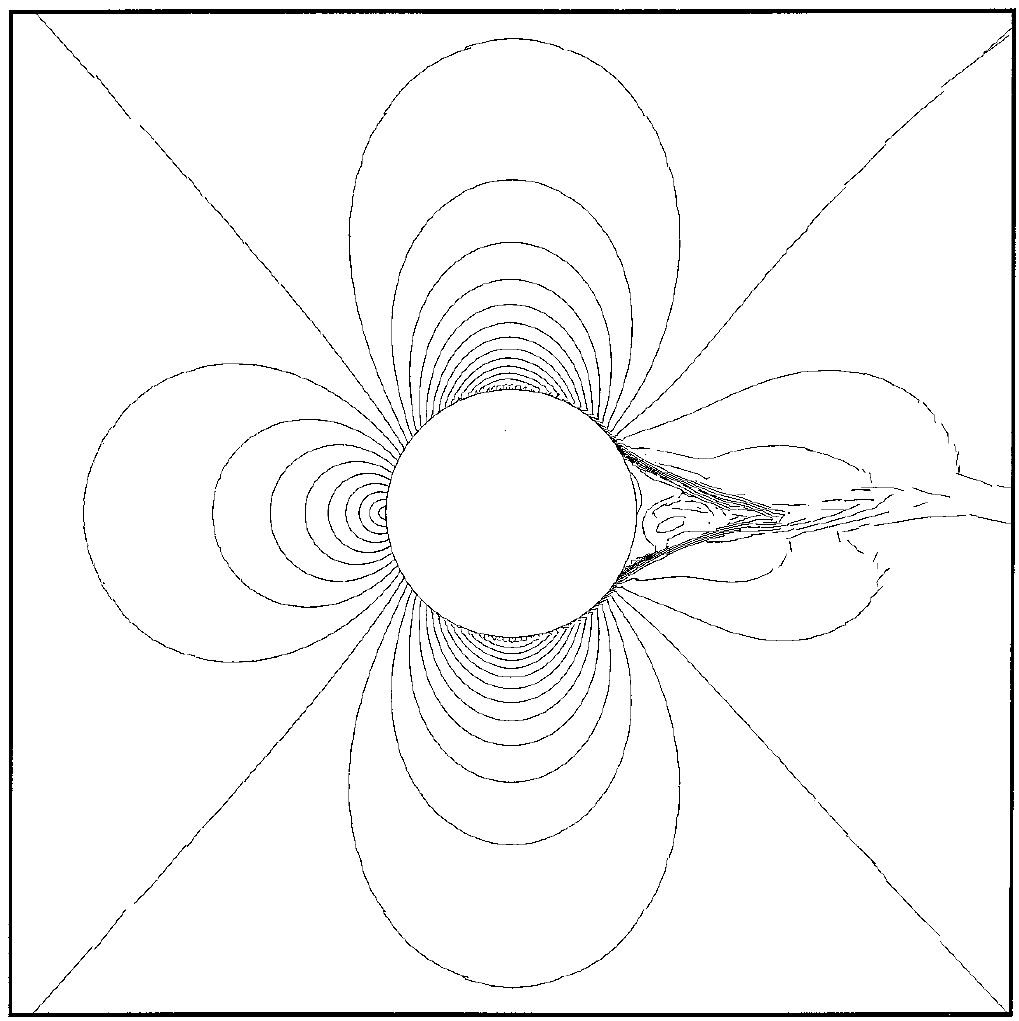
\includegraphics[scale=0.15]{bassi-linear}
 	}
 	\subfloat{
 		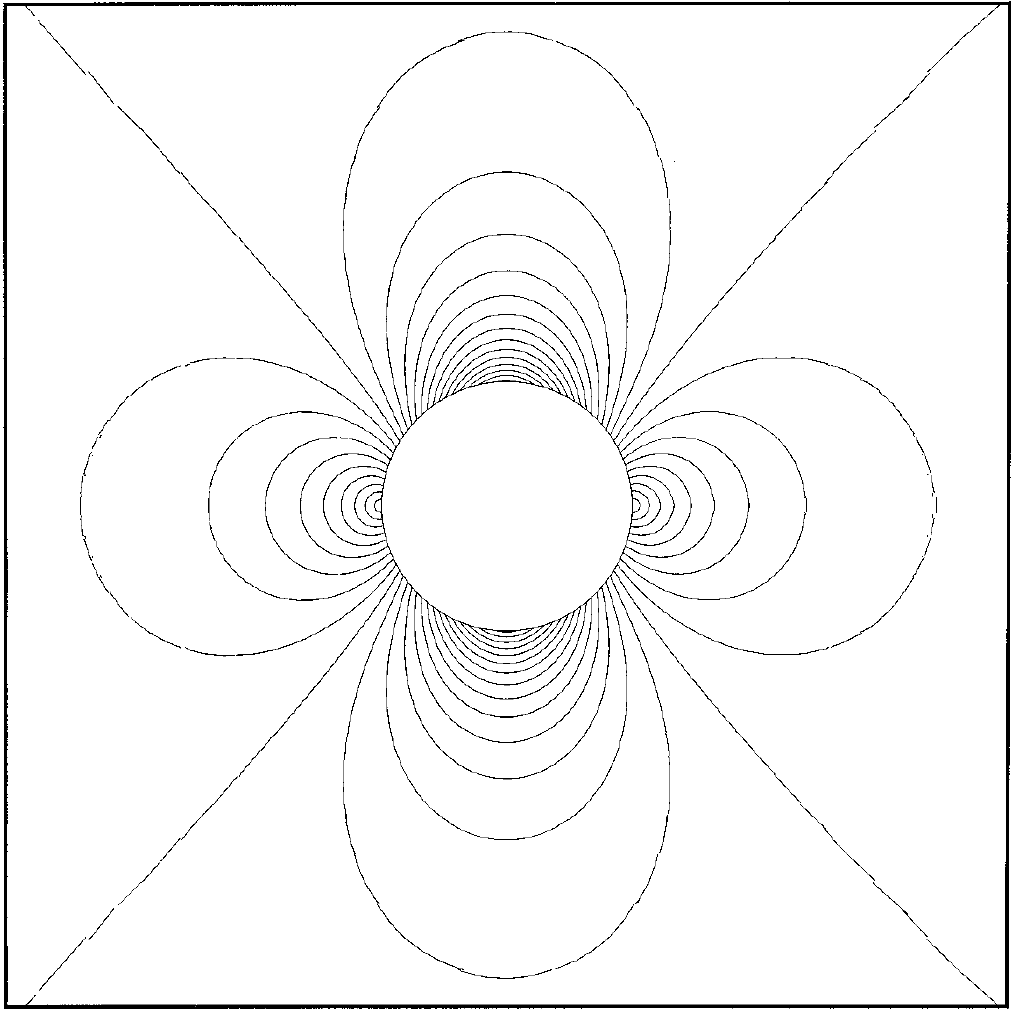
\includegraphics[scale=0.15]{bassi-q2}
 	}
 	\caption{Inviscid subsonic flow over a cylinder; left: DGP1 solution with regular linear mesh, right: DGP1 solution with quadratic (`Q2') mesh \cite{appl:dgeuler}}
 	\label{fig:bassi}
 \end{figure}
Thus, robust techniques to obtain a high-order representation of the geometry (the boundary of the domain) have become important.  One technique of high-order boundary approximation is to produce high-order meshes, otherwise called curved meshes. Another technique in this regard is isogeometric analysis \cite{isogeometric} where CAD data is directly used in analysis. In this work, we deal with curved unstructured mesh generation, using either CAD data if available, or only the linear mesh data. If only linear mesh data is available, a high-order boundary reconstruction is used to compute a higher order approximation, and the mesh is then curved according to this reconstructed boundary. Once the boundary is curved, regularization of the interior mesh is generally required to maintain mesh quality.

In chapter 3, the method of curved mesh generation adopted for this work is described. For regularizing the interior mesh, we prefer interpolation by radial basis functions (RBF) \cite{rbf:errorwendland}. We compare this method with the `stiffened' linear elasticity method \cite{mm:fsielast}. For our test cases, both are found to work quite well but the RBF method takes comparatively very little time.

Results for both mesh movement and curved mesh generation are presented in chapter 4. We conclude in chapter 5 with a comparison of the methods, and give some more details of our implementation in the appendices.

\chapter{Review of mesh movement methods}

 In our knowledge, there are, broadly speaking, three types of methods to achieve movement of the interior nodes knowing the movement of the boundary nodes. The first type uses models based on solid mechanics to try to achieve valid mesh movement. Examples of this type are lineal spring analogy \cite{mm:batina}, torsion spring analogy \cite{mm:torsionsprings}, linear-elasticity (and variants thereof)\cite{curve:hartmann} and non-linear elasticity \cite{curve:persson}. Each of these requires solution of a system of equations involving the same number of variables as mesh points to be moved. The linear-elasticity based models require solution of Poisson-type partial differential equations.
 
 The second type of technique to move the interior nodes involves \emph{interpolation} of the boundary displacement to interior nodes. Several methods exist; some examples are radial basis function (RBF) interpolation \cite{mm:rbf}, `explicit' interpolation \cite{mm:explicit}, and `Delaunay graph mapping' \cite{mm:dgm}. These methods do not involve any physics-based modeling of the mesh.
 
 \section{Elasticity methods}
 Elasticity-based methods are among the oldest mesh-movement methods in use. These include lineal spring analogy, torsional spring analogy, and various kinds of elastic solid mechanics analogies. These methods model the mesh as some kind of solid entity, impose a boundary displacement and solve equilibrium equations to propagate the motion to the interior nodes.
 
 \subsection{Spring analogies}
 
 Lineal spring analogy is the simplest method that can be used to move internal mesh points in response to movement of the boundary, invented by J.T. Batina. Each edge of the mesh is assumed to represent a lineal spring connecting the two nodes which make up the edge. The idea is that after imposing boundary movement, the mesh is allowed to ``go to equilibrium". At every mesh point, we have
 \begin{equation}
 \sum_j k_{ij}(\Delta \mathbf{r}_i - \Delta \mathbf{r}_j) = \mathbf{0} \quad \forall i
 \label{spring}
 \end{equation}
 where $i$ ranges over all nodes, $j$ ranges over points surrounding node $i$ and $\Delta \mathbf{r}_i$ is the displacement of node $i$.
 $k_{ij}$ is the stiffness of the spring between nodes $i$ and $j$, which can be taken as
 \begin{equation}
 k_{ij} = \frac{1}{||\mathbf{r}_i - \mathbf{r}_j||}.
 \end{equation}
 
 This method is not reliable as it generates invalid elements (having zero or negative value of the Jacobian determinant of the reference-to-physical element mapping) for even relatively small displacements, depending on the mesh. However, for the application it was developed, it sometimes gives acceptable results. It is used, for example, by Mavriplis \emph{et. al.} \cite{appl:mavriplis} in an optimization problem involving inviscid flow only. It is also less computationally expensive compared to other elasticity-based methods.
 
 Note that separate problems are solved in each coordinate direction, which are uncoupled. It is the author's opinion that this is the main reason for its unreliability for many kinds of mesh and movement combinations. However, because of this, extension to 3D is trivial.
 
 The torsional spring analogy is an extension to the previous method, which adds torsional springs at each node in each element (see Farhat \emph{et.al.} \cite{mm:torsionsprings}).
 These torsional springs resist the relative angular motion between edges of an element. This leads to a substantially more robust movement. In the scheme of Farhat \emph{et. al.}, the problem is divided into two parts, one related to lineal spring analogy and one to the torsional spring analogy. The lineal spring model is not the same as that used by Batina; in this case the lineal spring model also leads to a coupled system which is more robust than the uncoupled scheme. The torsional part adds even more resistance to invalid elements. As shown in figure \ref{f:torsion}, the torsional spring analogy adds torsion springs at each node of each element. The stiffness of a torsion spring associated with a node of a certain element is a function of the angle formed by the edges of that element meeting at the node.
 
 \begin{figure}
 	\centering
 	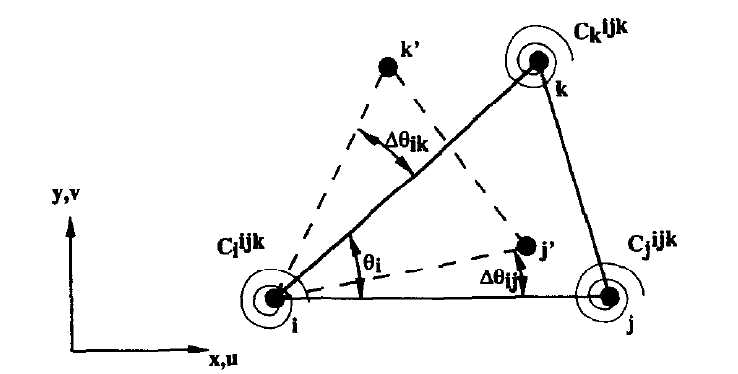
\includegraphics[scale=0.25]{torsionspring}
 	\caption{Movement of an element in torsion spring analogy; from \cite{mm:torsionsprings}}
 	\label{f:torsion}
 \end{figure}
 
 While this method is significantly more robust than the lineal spring analogy of Batina, it is also much more computationally expensive. A fully coupled system of $n_{dim} N_n$ equations must be solved, where $N_n$ is the number of nodes that are to be moved in the mesh and $n_{dim}$ is the dimension of the problem.
 
 \subsection{Elastic solid analogy (`Elasticity')}
 
 The deformable elastic solid analogy, employing the equations of (linear or non-linear) elasticity, is one of the widely-used mesh movement techniques. This class of schemes often lead to very robust mesh movement. The mesh is assumed to model a deformable solid body, which is then deformed according to the equations of solid mechanics, that is, linear or non-linear elasticity.
 
 \subsubsection{Linear elasticity}
 
 The simplest approach is linear elasticity.
 \begin{equation}
 \nabla \cdot \mathbf{\sigma}  = \mathbf{0} \quad \text{in} \, \Omega
 \end{equation}
 Assuming an isotropic material, the constitutive relation can be taken as
 \begin{equation}
 \bld{\sigma} = 2\mu\bld{\epsilon} + \lambda (\mathrm{tr}\boldsymbol{\epsilon}) \bld{I}
 \label{linelast:constt}
 \end{equation}
 where $\bld{\sigma}$ is the stress and $\bld{\epsilon}$ is the strain.
 Finally, the linear strain-displacement relation is given by
 \begin{equation}
 \bld{\epsilon} = \frac12 (\nabla\bld{u}+\nabla\bld{u}^T)
 \label{linelast:strain}
 \end{equation}
 where $\bld{u}$ is the displacement field, with Dirichlet boundary conditions (prescribed boundary displacement $\bld{u}_b$)
 \begin{equation}
 \bld{u} = \bld{u}_b \quad \text{on} \, \partial\Omega
 \end{equation}
 The weak form of this set of equations, solved by Galerkin finite element method (FEM) leads to a linear system of size $n_d N_n$, where $n_d$ is the dimension of the problem and $N_n$ is the number of nodes to be moved.
 
 \subsubsection{`Sitffened' linear elasticity}
 \label{subsec:stiffelast}
 While the basic linear elasticity scheme is adequate for some applications, it is not adequate for stretched, boundary-layer meshes for viscous flow, among others. The scheme is often modified by `stiffening' the mesh appropriately, so as to attain some control over the propagation of deformation into the interior of the mesh, as done, for instance, by Hartmann and Leicht \cite{curve:hartmann}. In their work, the material is stiffened based on the determinant of the local Jacobian matrix of the reference-to-physical mapping, that is to say smaller elements are stiffer than larger ones. If $\hat{\kappa}$ is the reference element corresponding to the physical element $\kappa$, the local bilinear form on $\kappa$ giving rise to the local stiffness matrix 
 \begin{equation}
 (\dots)_\Omega = \sum_{\kappa \in T_h} \int_{\kappa} \dots d\mathbf{x} = \sum_{\kappa \in T_h} \int_{\hat{\kappa}} \dots J_\kappa d\mathbf{x}
 \end{equation}
 is modified according to
 \begin{equation}
\int_{\hat{\kappa}} \dots J_\kappa d\mathbf{x} \text{becomes} \int_{\hat{\kappa}} \dots J_\kappa \left(\frac{J_0}{J_\kappa}\right)^\chi d\mathbf{x}
 \end{equation}
 where $J_\kappa$ is the Jacobian of the reference-to-physical mapping of the element $\kappa$, $J_0$ is a reference Jacobian for the mesh and $\chi$ is an constant to be chosen.
 
 \subsubsection{Nonlinear elasticity}
 
 Nonlinear elasticity is claimed to be a highly robust method for mesh movement by Persson and Peraire \cite{curve:persson}. As long as the mesh is fine enough to resolve the displacements, they claim that element validity is guaranteed. In their work, for non-linear elasticity, the constitutive equation \eqref{linelast:constt} and strain-displacement relation \eqref{linelast:strain} are replaced by the `neo-Hookean' constitutive model
 \begin{equation}
 \bld{P} = \mu ((\boldsymbol{F}^T\bld{F})\bld{F}^{-T} - \bld{F}^{-T}) + \lambda(\ln \det\bld{F})\bld{F}^{-T}
 \end{equation}
 where the deformation gradient $\bld{F}$ is given by
 \[
 \bld{F} = \frac{\partial\bld{x}}{\partial\bld{X}}.
 \]
 Here, $\bld{x}$ is the physical position vector of a point with coordinate $\bld{X}$ in the reference configuration. The system is solved using Newton-GMRES iterations.
 
 In our opinion, this method probably cannot be used in any unsteady moving-geometry simulations, as the cost will be prohibitive. However, it leads to good results for curved mesh generation, as can be seen in Persson and Peraire's work.
 
 The advantage of elasticity-based methods is that they can be made highly robust. Their disadvantage is that generally, the more robust the scheme, the more expensive it is. The cost of the system of equations that needs to be solved usually scales with the total number of mesh nodes to be moved; this can get very expensive for 3D viscous meshes. Further, the implementation is usually not very easy; different cell types require different treatments (different basis functions, for instance, in case of elastic-solid approaches) and extension from 2D to 3D may not be trivial (as in case of torsional springs).
 
 \section{Interpolation  Methods}
 Also called algebraic methods, these methods do not involve any physics-based modeling of the mesh. They are purely mathematical manipulations of the mesh. Unlike elasticity-based methods, schemes of this type tend to be fast and independent of mesh topology. 
 
 \subsection{Delaunay graph mapping (DGM)}
 \label{sec:dgm}
 Developed by Liu, Qin and Xia \cite{mm:dgm}, DGM is a fast method of mesh movement. It consists of the following steps.
 \begin{itemize}
 	\item A Delaunay triangulation is constructed from the boundary points of the mesh. This triangulation is referred to as the Delaunay graph.
 	\item Each internal mesh point is located in the Delaunay graph, and its barycentric coordinates are calculated with respect to the Delaunay element it lies in.
 	\item Using the prescribed boundary displacements, the Delaunay graph is moved.
 	\item Using the calculated barycentric coordinates, the interior mesh points are mapped back to the deformed Delaunay elements keeping the barycentric coordinates constant, thus moving the mesh.
 \end{itemize}
 Thus, no linear system needs to be solved. The bulk of the work is in computing the Delaunay triangulation and traversing it, which can be done efficiently. We use the Bowyer-Watson algorithm to compute the Delaunay tessellation of the boundary points in both 2D and 3D \cite{bowyer}. Details of the exact algorithm used are provided in appendix ******A*******.
 
 This method results in a valid mesh as long as the boundary displacement does not invalidate the Delaunay graph itself. If the Delaunay graph becomes invalid, the displacement must be carried out in several steps. The Delaunay graph is re-computed each step, and thus much more boundary movement is possible without invalidating the sequence of Delaunay graphs.
 
 In our experiments, Delaunay graph mapping is not very robust when it comes to rotational motion, or otherwise very large deformation (see the results section).
 
 \subsection{Radial basis functions}
 
 Radial basis functions (RBFs) are radially-symmetric functions. They are used as a basis for the displacement field in the moving mesh \cite{mm:rbf}. Considering $n_b$ boundary points in the mesh, we express the displacement as
 
 \begin{equation}
 \mathbf{s}(\mathbf{x}) = \sum_{j=1}^{n_b} \mathbf{a}_j \phi(\lVert\mathbf{x} - \mathbf{x}_{bj}\rVert)
 \label{eqn:rbf}
 \end{equation}
 where $\mathbf{s}$ represents the displacement field, $\mathbf{x}$ is the position vector of any point in the domain, $\mathbf{x}_{bj}$ is the position of the $i$th boundary point, $\phi$ is a radial basis function, $\phi(\lVert\mathbf{x} - \mathbf{x}_{bj}\rVert)$ is the $j$th basis function for the displacement field, and $\mathbf{a}_j$ is the $j$th coordinate or coefficient in that basis.
 
 Since we know the displacements of the boundary nodes, we can solve for the coefficients $\mathbf{a}_j$ using
 \begin{equation}
 \mathbf{s}(\mathbf{x}_{ib}) = \sum_{j=1}^{n_b} \mathbf{a}_j \phi(\lVert\mathbf{x}_{bi} - \mathbf{x}_{bj}\rVert).
 \end{equation}
 
 In each coordinate direction, this leads to a system of $n_b$ equations in $n_b$ unknowns:
 \begin{equation}
 \mathbf{A}\mathbf{a}_k = \mathbf{s}_k
 \end{equation}
 where the $(i,j)$ component of $\mathbf{A}$ is $\phi(\lVert\mathbf{x}_{bi} - \mathbf{x}_{bj} \rVert)$, $ \bld{a}_k \in \mathbb{R}^{n_b}$ is the coefficient vector in the $k$th direction and $\bld{s}_k \in \mathbb{R}^{n_b}$ is the vector of boundary displacements in the $k$th coordinate direction.
 
 In our implementation, we assemble $\mathbf{A}$ as a sparse matrix by evaluating the radial basis function between every pair of boundary points. This process can be parallelized easily.
 
 Next, we need to evaluate equation \eqref{eqn:rbf} for each interior point, which requires one evaluation of the RBF for each interior point (in each direction). This too, can be parallelized easily.
 
 The quality of the final mesh depends on which RBF is used. Many kinds of RBFs have been used in literature \cite{mm:rbf, mm:rbf2}. In this work, we use Wendland's C2 function
 \begin{equation}
 \phi(x) = (1-x)^4(4x + 1),
 \end{equation}
 or rather, a modification,
 \begin{equation}
 \phi(x) = 
 \begin{cases}
 \left(1-\frac{x}{r_s}\right)^4\left(4\frac{x}{r_s} + 1\right) & x < r_s \\
 0 & x \geq r_s
 \end{cases}
 \end{equation}
 where $r_s$ is a real number called the `support radius'. This modified function has a compact support. In light of this, we see the matrix $\mathbf{A}$ is sparse if the support radius is less than the characteristic dimension of the domain. For curved mesh generation, this support radius can be kept quite small relative to the whole domain, giving us a very sparse linear system which is solved quite fast.
 
 The scaling of the argument by the support radius serves to make the value of the RBF 1.0 at the boundary. This means that points very close to the boundary will deform just like the boundary itself. This results in an essentially rigid motion of points very close to the boundary, which causes the near-boundary elements to retain their quality after the mesh movement. The support radius is chosen big enough to accommodate the expected deformation of the boundary, but small enough that the linear system is sparse. An algorithm to determine a good support radius will be very useful in this regard.
 
 The RBF method can be carried out in multiple steps; this is found to increase the quality of generated meshes in some cases involving large rotational deformations (\ref{fig:wing-inviscid-rbf}), but not so much in others, such as curved mesh generation.
 
 \subsection[DG-RBF]{Interpolation using radial basis function on the Delaunay graph (DGRBF)}
 This method proposed by Wang, Qin and Zhao \cite{mm:dgrbf} combines both the Delaunay graph mapping and interpolation by RBF. The general scheme of the mesh movement is the same as in case of DGM, but with the important difference that interpolation is not done using barycentric coordinates of the nodes with respect to the Delaunay graph elements. Here, the interpolation is done via radial basis functions in each Delaunay graph element. The displacement of a node with initial position $\bld{x}$ is given by
 \begin{equation}
 \mathbf{s}(\mathbf{x}) = \sum_{j=1}^{n_t} \mathbf{a}_j \phi(\lVert\mathbf{x} - \mathbf{x}_{tj}\rVert)
 \label{eqn:dgrbf}
 \end{equation}
 where $\bld{x}_{tj}$ are positions of nodes of the Delaunay simplex that contains the node at $\bld{x}$, and $n_t$ is the number of nodes in that simplex (3 in 2D and 4 in 3D). We need to solve for the $\bld{a}_j$, the RBF coefficients, by solving a $3 \times 3$ system in 2D or a $4 \times 4$ system in 3D, in each Delaunay element.
 \begin{equation}
 \mathbf{s}(\mathbf{x}_{ti}) = \sum_{j=1}^{n_t} \mathbf{a}_j \phi(\lVert\mathbf{x}_{ti} - \mathbf{x}_{tj}\rVert).
 \label{eqn:dgrbfsys}
 \end{equation}
 
 DGRBF method provides flexibility in choosing the RBF and the support radius, and with a good choice of these, robust mesh movement can be achieved for translational motion and possibly some other kinds of deformation. It has been observed in \cite{mm:dgrbf} and in our tests, that interpolation of displacements by DGRBF often does not give very good results for large rotational deformations. The remedy for this is to interpolate the rotational angles instead of the displacements directly, and then calculate the displacements at each interior node using these interpolated rotation angles using the rotation matrix. For example, in 2D,
 \begin{align}
 x_{new} &= (x-x_0)\cos a_z - (y-y_0)\sin a_z + x_0 \\
 y_{new} &= (x-x_0)\sin a_z + (y-y_0)\cos a_z + y_0
 \end{align}
 where $(x_0,y_0)$ is the center of rotation, and $a_z$ is the interpolated rotation angle at the node in question. For interpolation of the angles, the same formulae \eqref{eqn:dgrbf} and \eqref{eqn:dgrbfsys} are used, with the rotation angles replacing the displacements. Angle interpolation can be combined with displacement interpolation for problems involving both translation and rotation. This angle interpolation scheme, and its combination with the displacement interpolation scheme, is referred to as `DGRBF2' in \cite{mm:dgrbf}.
 
 \subsection{`Improved' Delaunay graph mapping}
 \label{sec:hybriddg}
 If the Delaunay graph (DG) lines are not approximately normal to the boundary, there can sometimes be issues with mesh movement. Mesh lines tend to be normal to the boundary for physical and numerical reasons. If Delaunay graph lines make very small or very large angles (compared to 90 degrees) with the boundary, successive interior nodes on the same mesh line can lie in different DG triangles. This would cause non-smooth displacement of interior mesh nodes; an example is presented in detail in section \ref{subsec:dgmunsuitable}.
 
 One way of improving this method, that was considered by the author and Dr Hong Luo, was to include a few interior mesh points in the Delaunay graph such that the Delaunay graph lines stayed approximately normal to the boundary near it. For example, a layer of nodes could be chosen around each component of a 3-component airfoil such that each airfoil boundary gets approximately normal Delaunay graph lines. This method would require movement of the interior Delaunay graph nodes by a different method, such as RBF or linear elasticity. Since the number of these interior nodes in the Delaunay graph is very small, solution of the RBF or linear elasticity problems could be done quickly.
 
 % ADD PICTURE HERE
 
 Xiao et. al. present a very similar method \cite{mm:hybriddg}. Instead of choosing interior Delaunay graph points from among the interior mesh points, they generate a `background' coarse mesh to serve as the Delaunay graph (DG). The motion of the DG is obtained using Batina's lineal spring analogy method \cite{mm:batina}.
 
 \section{Linear Mesh quality}
 \label{sec:lin-mesh-quality}
 In order to judge the effectiveness of mesh-movement methods, we need to measure the quality of the deformed mesh. Some mesh quality measures have been derived for linear 2D and 3D elements by Knupp \cite{qualknupp}. These include the relative size, shape and size-shape metrics for triangles and tetrahedra, and size, shape, skew, size-shape and size-skew metrics for quadrangles and hexahedra.
 
 The size metric distinguishes elements having very small or very large volume with respect to some reference volume. The shape metric identifies elements that have unequal edges or unequal angles between edges; it is independent of size of the element. Finally, the skew metric is a measure of unequal angles between edges of the element only, irrespective of lengths of edges and volume of element. The skew metric is different from shape in case of non-simplicial (like quadrangular and hexahedral) elements. While dealing with quadrilaterals, we use the skew metric. This is because for boundary layer meshes, cells with high aspect-ratios are desired, but they have poor shape metric. For triangular meshes, cells with high aspect-ratio must have very unequal interior angles too, leaving no difference between shape and skew.
 
 All metrics are normalized so that they are 1.0 for ideal elements with regard to the characteristic they measure, and they are 0.0 for degenerate elements. 
 

\chapter{Curved mesh generation}
\section{Introduction}

The problem of curved mesh generation involves at least one issue - the placement of the boundary ``high-order" nodes. A description of a high-order boundary is required, and the optimal placement of high-order boundary nodes must be decided.

Additionally, we usually need to deal with one more issue - maintaining the quality of elements near the boundary after placing the high-order boundary nodes. The deformation of the initially polygonal/polyhedral boundary to get a curved boundary usually causes the quality of boundary elements to get reduced. In cases with a viscous boundary layer mesh, these elements even become invalid \cite{curve:persson, gmsh:untangling}. Thus, the deformation of the boundary must be propagated into the domain, to displace interior nodes upto at least some distance from the boundary.

In our knowledge, there are three types of methods to achieve regularization of the interior mesh. The first type uses models based on solid mechanics to try to achieve valid mesh movement, as explained in the previous chapter. The second type of technique to move the interior nodes involves interpolation of the boundary displacement to interior nodes, again, as previously explained. An interesting development in curved mesh generation by interpolation is due to Ims at. al. \cite{curve:meshcurve}, in which explicit interpolation (\cite{mm:explicit}) is used to curve the interior of the mesh. Finally, researchers have ``untangled" the near-boundary elements, and otherwise improved the quality of the mesh, by optimization processes. The cost function is usually some kind of curved-mesh quality measure. One prominent example of this is in the Gmsh meshing software \cite{gmsh:untangling}.

We present an alternative approach based on interpolation by radial basis functions. This approach is compared to the more prevalent methods of linear elasticity \cite{curve:hartmann}.

In the rest of the sections, we discuss the methodology used to generate 2D unstructured quadratic meshes from linear meshes, and then present examples to demonstrate the effectiveness of our method. We compare the quality of meshes given by the RBF interpolation method and the linear-elasticity method.

We initially preprocess the linear mesh to generate a straight-faceted high-order mesh. To do this, we introduce extra nodes along edges, in faces and inside cells as required. Next, we either use CAD data or use a high-order boundary reconstruction method to obtain the actual positions of boundary high-order nodes. Finally, interior nodes are moved according to the boundary displacement imposed because of the previous step.

\section{Spline reconstruction for boundaries of 2D meshes}
\label{subsec:spline2d}
If only the linear mesh is taken as input, a high-order boundary representation first needs to be reconstructed from the piecewise linear $C^0$ boundary. For 2D meshes, we use a cubic spline reconstruction to get a smooth ($C^2$) parametric curve describing the boundary. All boundary nodes are used as spline control points, and we get a cubic function between every two consecutive boundary nodes. At the control points, we require the two spline curves meeting there to share a common tangent and curvature, thus enforcing $C^2$ continuity. Since it is common for the true boundary to be specified in terms of cubic spline curves, this is expected to give us an accurate reconstruction. Corners are detected by comparing the normal vectors of the two facets sharing a point. If the dot product between the two normal vectors is below a particular user-specified threshold, the point is considered as a corner and is not smoothed over by the reconstruction procedure. Alternatively, the user can list all the corner points as input. Thus the reconstructed boundary is piecewise $C^2$, which is found to work well for the test cases we considered. The spline reconstruction requires the solution of a symmetric positive definite linear system, of size equal to the number of boundary nodes in the curved part of the boundary, in order to calculate the cubic spline coefficients. The system(s) can be solved quickly using a conjugate gradient (CG) solver. More details are given in appendix \ref{app:spline}.

Instead of a global reconstruction by cubic splines, a local reconstruction at each boundary node could also be used. This is described briefly for 3D meshes in the last chapter, conclusions and future work.

Once we have the smooth reconstructed boundary, we calculate the final positions of the boundary nodes in the curved mesh. This is currently done by simply moving the high-order boundary nodes, originally at regular intervals on the boundary facet, to corresponding intervals in parameter space on the cubic spline curve associated with that facet. This method is found to be quite robust for the meshes tested. Thus, the boundary displacements are obtained. Alternatively, if the CAD geometry is available, the displacements can be computed using it.

\section{Interior mesh movement}

To propagate the boundary motion to the interior of the mesh, we favor interpolation by radial basis functions (RBFs) \cite{mm:rbf}. We have also used linear elasticity to propagate the mesh movement to the interior. The isotropic linear elasticity variational formulation, as given by Gockenbach \cite{gockenbach}, is implemented in a P2 Galerkin FEM code for generation of quadratic meshes. In this case however, the size of the linear system to be solved is proportional to the total number of nodes in the mesh.

Though the RBF method requires the solution of a linear system of size proportional to only the number of boundary points, extra computation is required to evaluate equation \eqref{eqn:rbf} at each of the interior nodes to compute their displacements. In comparison, elasticity-based methods directly give us the displacements. 

While solving certain problems with the RBF method, we find that the linear system to be solved is sometimes quite ill-conditioned, depending upon the mesh. Iterative Krylov-subspace solvers such as conjugate gradient (CG) and BiCGSTAB are not able to solve the system in such cases. However, in the cases that we worked on (such as curved mesh generation of hybrid meshes for viscous simulations of airfoils), sparse direct methods are capable of solving the system efficiently and effectively. This is likely to hold true in general as the systems to be solved will usually not be very large (having size of the number of boundary nodes).

The inability of iterative solvers to compute a solution can perhaps be explained by the discussion on condition numbers of RBF matrices in Wendland's paper \cite{rbf:errorwendland}. If
\begin{equation}
q := \min_{i\neq j} \lVert \bld{x}_{bi} - \bld{x}_{bj} \rVert_2
\end{equation}
is the minimum distance between two boundary points, and $\bld{A}$ is the RBF interpolation matrix \eqref{eqn:rbf_system} then for Wendland's C2 function, we will have
\begin{equation}
\begin{aligned}
\text{cond}_2 (\bld{A}) &= \mathcal{O}(q^{-5}) \quad \text{in 2D, and} \\
\text{cond}_2 (\bld{A}) &= \mathcal{O}(q^{-6}) \quad \text{in 3D}
\end{aligned}
\end{equation}
as seen from section 4 of \cite{rbf:errorwendland}. In the case that the CG solver did not work, we had a 2D mesh with $q \approx 4 \times 10^{-7}$. This means that the condition number can be as high as $10^{30}$! Since we used only point-Jacobi preconditioning, we expect CG to not work in this case. If a more potent preconditioner (such as incomplete Cholesky decomposition or LU-SGS \cite{lusgs_precon}) is used, CG might be expected to work. But we found that direct solvers such as sparse LU decomposition work very well, and adopted this instead.

We have also tried using the stiffened linear elasticity method described in subsection \ref{subsec:stiffelast}. In this work, this is implemented by scaling each component of the element stiffness matrix of element $\kappa$ by the scaling term $\left(\frac{J_0}{J_\kappa}\right)^\chi$. This is valid as we only need to run the linear elasticity code on straight-sided meshes, and this means that the Jacobian determinant $J_\kappa$ is constant over the element.

\subsection[Unsuitability of DG-based methods for curved mesh generation]{Unsuitability of Delaunay-graph-based methods for curved mesh generation}
\label{subsec:dgmunsuitable}
%********* TODO: DESCRIBE WHY DGM AND DG-RBF FAIL FOR CURVED MESH GENERATION. DESCRIBE THE 2-STEP RBF-DG METHOD, AND WHY THAT DOES NOT WORK EITHER *********

Several variants of the Delaunay graph mapping method were also attempted for generating curved meshes. While Delaunay graph mapping (DGM) is a very efficient scheme for accomplishing many types of mesh movement, it has a characteristic because of which it is unsuitable for certain meshes and motions, especially curved mesh generation. This is the fact that the movement of a node depends only on the motion of the Delaunay element containing it, not necessarily on the motion of the nearest boundary facets.

In case of curved mesh generation for highly anisotropic viscous meshes, it is possible for some Delaunay triangulation facets to make angles with the boundary that are very different from 90 degrees (see figure \ref{fig:wmesh-dg}). Then we may have at least two issues.
\begin{itemize}
	\item[1.] Interior points close to a boundary facet can be influenced by another boundary facet far away having a very different curvature.
	\item[2.] It may be the case that an interior point is not at all influenced by the closest boundary facet.
\end{itemize}
These issues lead to low curved mesh quality in certain regions, and even invalid elements. We could try using DG-RBF (interpolation by radial basis functions in a Delaunay graph) to help alleviate issue (1), but issue (2) would still persist.

Figure \ref{fig:wmesh} shows a viscous mesh of a 3-element airfoil. Figures \ref{fig:wmesh-dg} and \ref{fig:wmesh-zoomed} show a portion of its slat. Figure \ref{fig:wmesh-dg} shows the Delaunay graph and figure \ref{fig:wmesh-zoomed} shows the deformed mesh. We can see that the DG lines make an angle very different from 90 degrees with the boundary. It is clear how points originally in a straight line deform in an oscillatory manner because successive points depend on different Delaunay elements, and different Delaunay elements have different movements depending on which boundary nodes they are made up of.

\begin{figure}
	\centering
	\includegraphics[scale=0.28]{3-airfoil}
	\caption{Mesh of a 3-element airfoil}
	\label{fig:wmesh}
\end{figure}
\begin{figure}
	\centering
	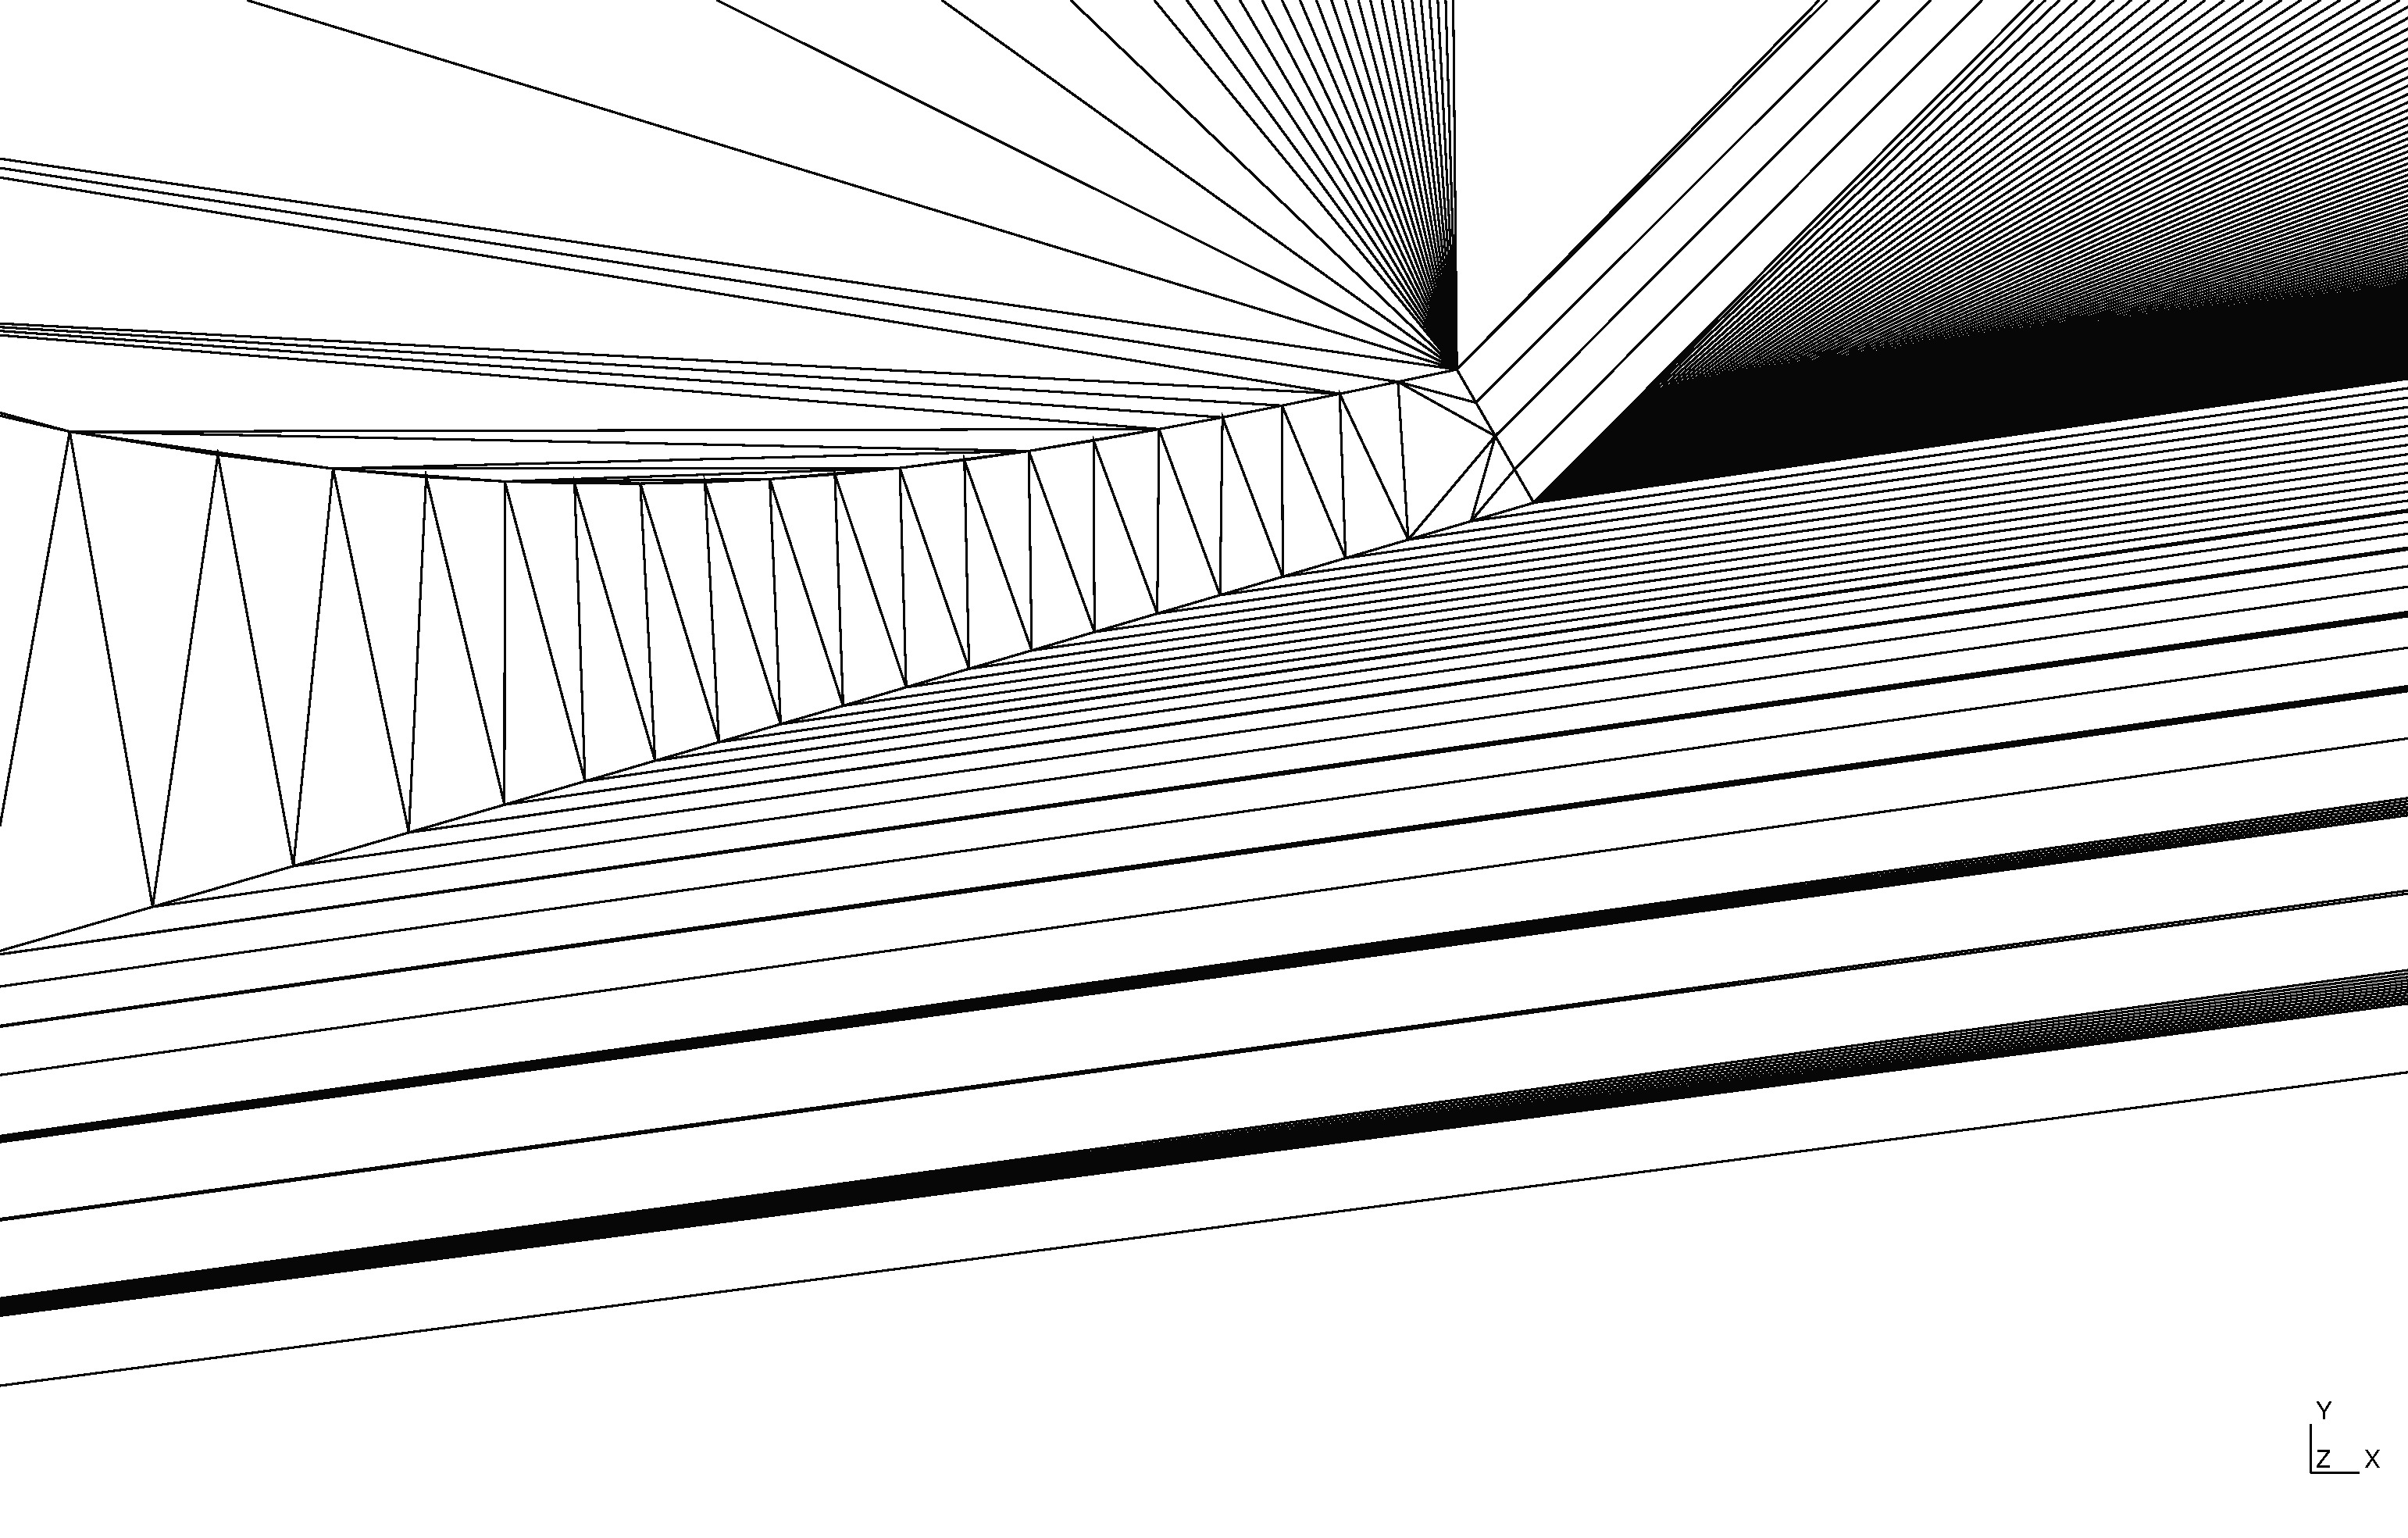
\includegraphics[scale=0.2]{dg-3airfoil-zoomed}
	\caption{Portion of the Delaunay graph near the lower part of the slat}
	\label{fig:wmesh-dg}
\end{figure}
\begin{figure}
	\centering
	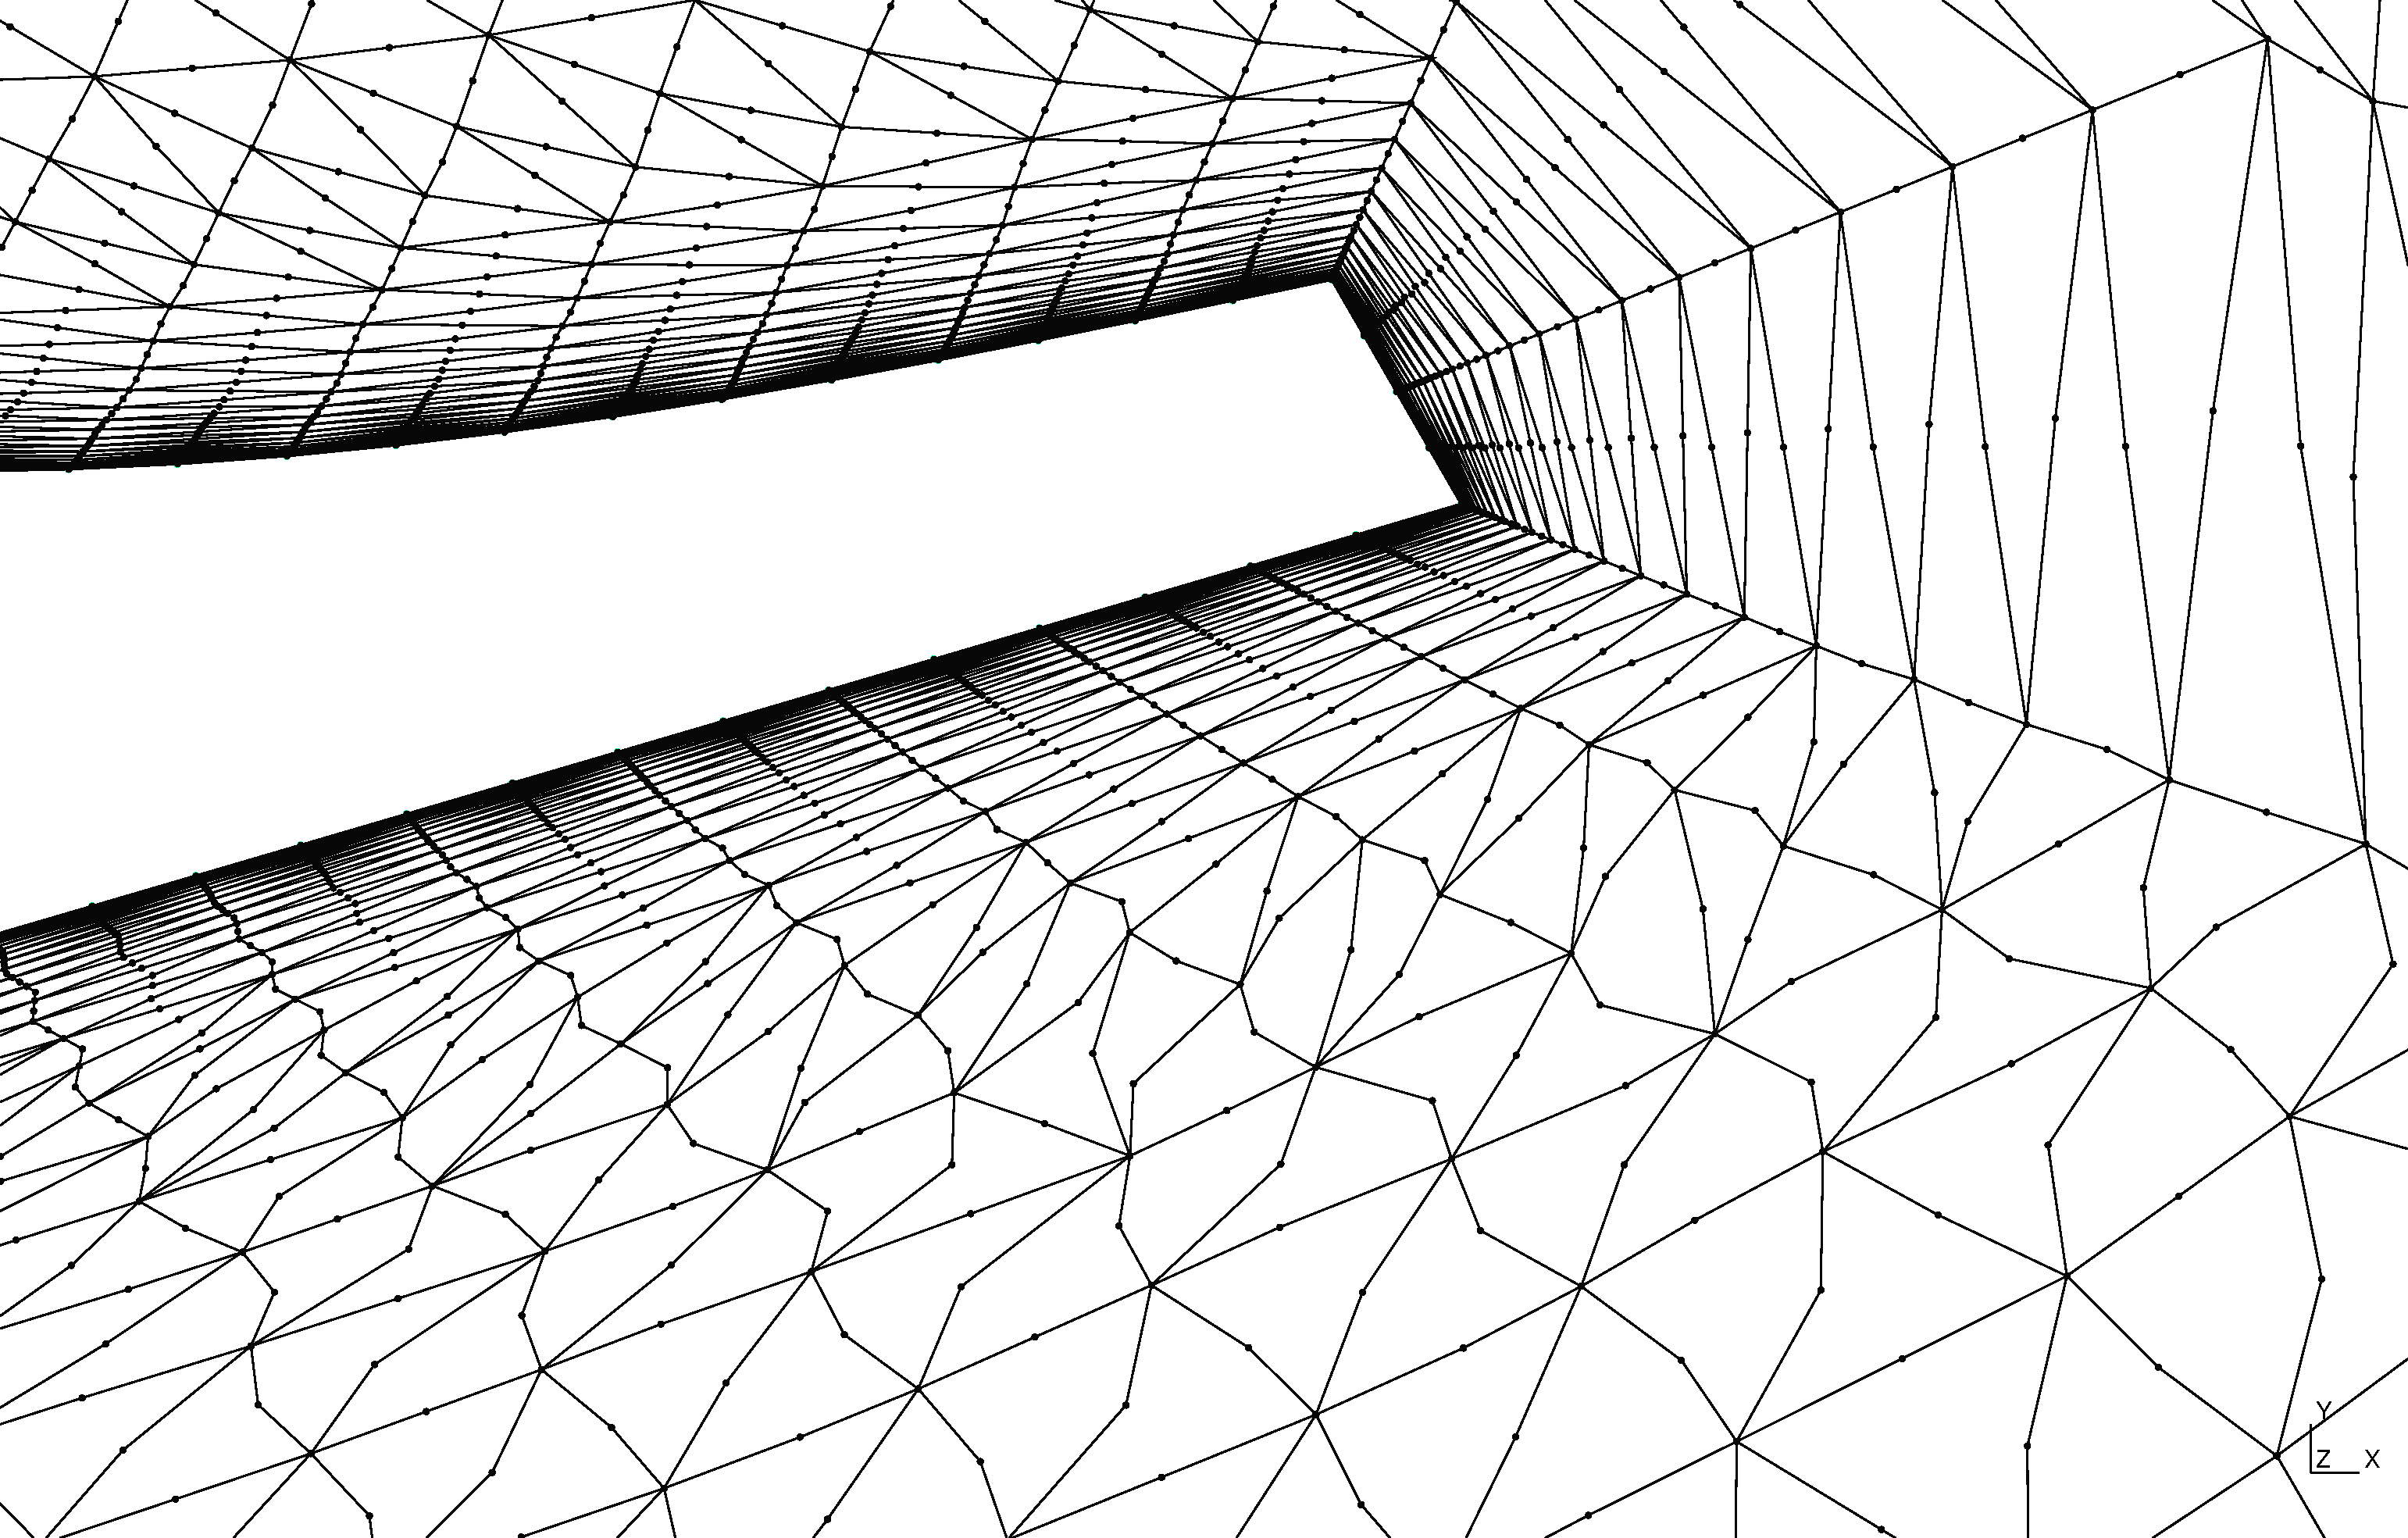
\includegraphics[scale=0.2]{mesh-3airfoil-zoomed}
	\caption{Portion of the generated mesh near the lower part of the slat}
	\label{fig:wmesh-zoomed}
\end{figure}

One way of improving this situation has been described in section \ref{sec:hybriddg}. However, the method of including a layer of interior points still does not work for curved mesh generation. This is simply to due to the high-frequency oscillatory nature of boundary displacements required for curved mesh generation and the fact that it is difficult to control how exactly the Delaunay graph (DG) elements are formed. It was found that some DG elements are formed by \emph{two high-order} boundary nodes and one interior node, as shown in figure \ref{fig:dg-curved-problem}. In the case shown, some interior nodes near the red circles (red circles are linear mesh nodes, called vertices) lie within a DG element that has nothing to do with the nearest boundary node, which is a boundary vertex in this case. A few interior nodes nearest to the boundary vertices are not inside the DG element, so they do not move because of the motion of the boundary high-order nodes. But beyond a small distance, the mesh nodes are in the DG element formed from two nearby high-order boundary nodes. This means that these nodes move with the DG element, and this creates a discontinuity in the interior node movement, leading to a bad boundary layer mesh.
\begin{figure}[!h]
	\centering
	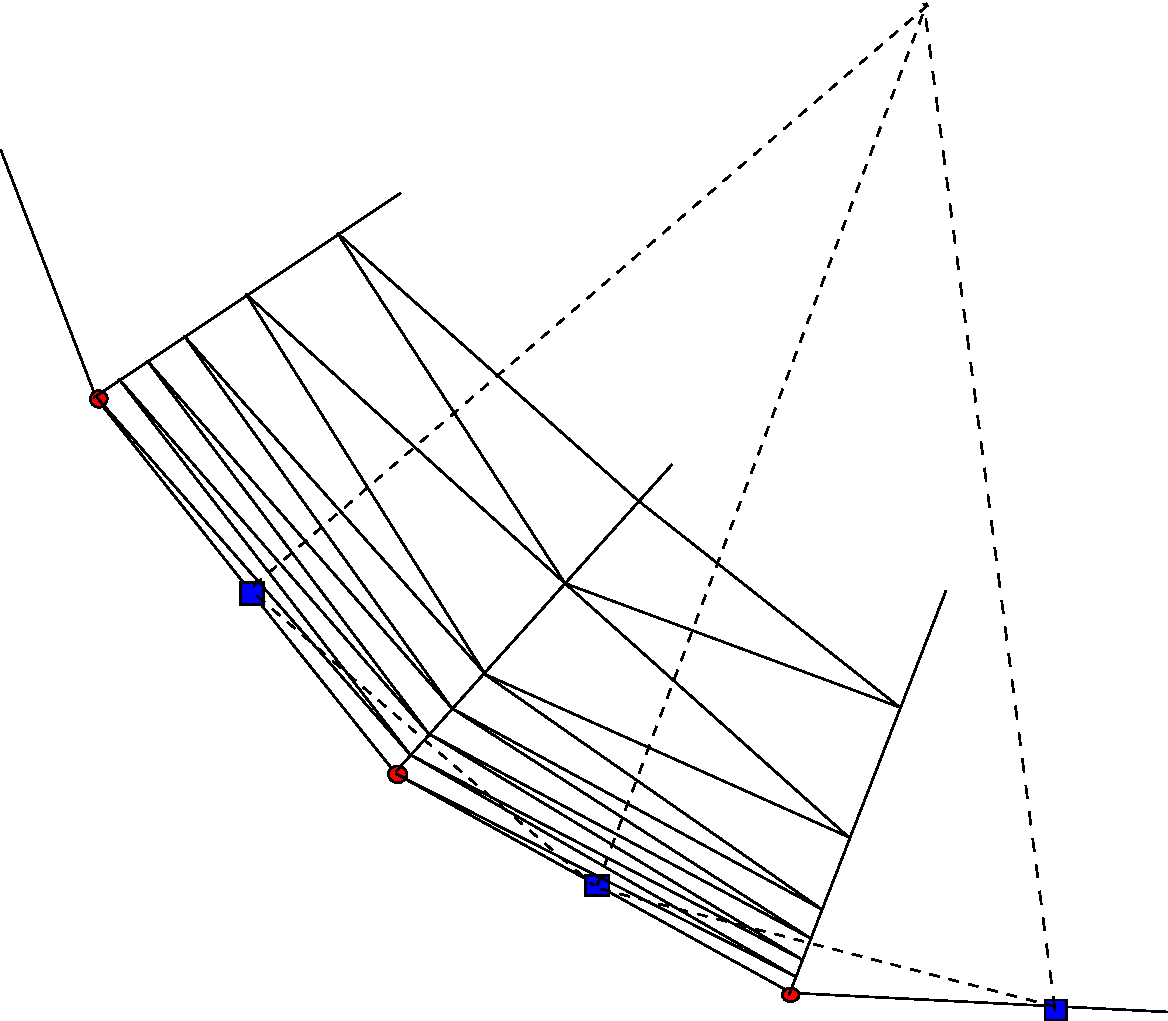
\includegraphics[scale=0.25]{DG-curved-problem}
	\caption{Schematic diagram to show a possible Delaunay graph (dashed lines) and mesh (solid lines) near a boundary; circles represent regular boundary nodes; squares represent high-order boundary nodes}
	\label{fig:dg-curved-problem}
\end{figure}
\chapter{Results}
 
\section{Mesh movement}
 
First, we show qualitatively the results for large deformation of a 2D unstructured linear mesh. In figure \ref{fig:wing-inviscid}, we show the undeformed mesh. In each of the results that follow, the flap of the wing has been rotated anti-clockwise by 60 degrees. We take note of the quality of triangular cells in these results. By `quality', we mean deviation of the angles of the triangle from 60$^\circ$, that is, the shape metric (sec. \ref{sec:lin-mesh-quality}), for this test case.
\begin{figure}
  	\centering
  	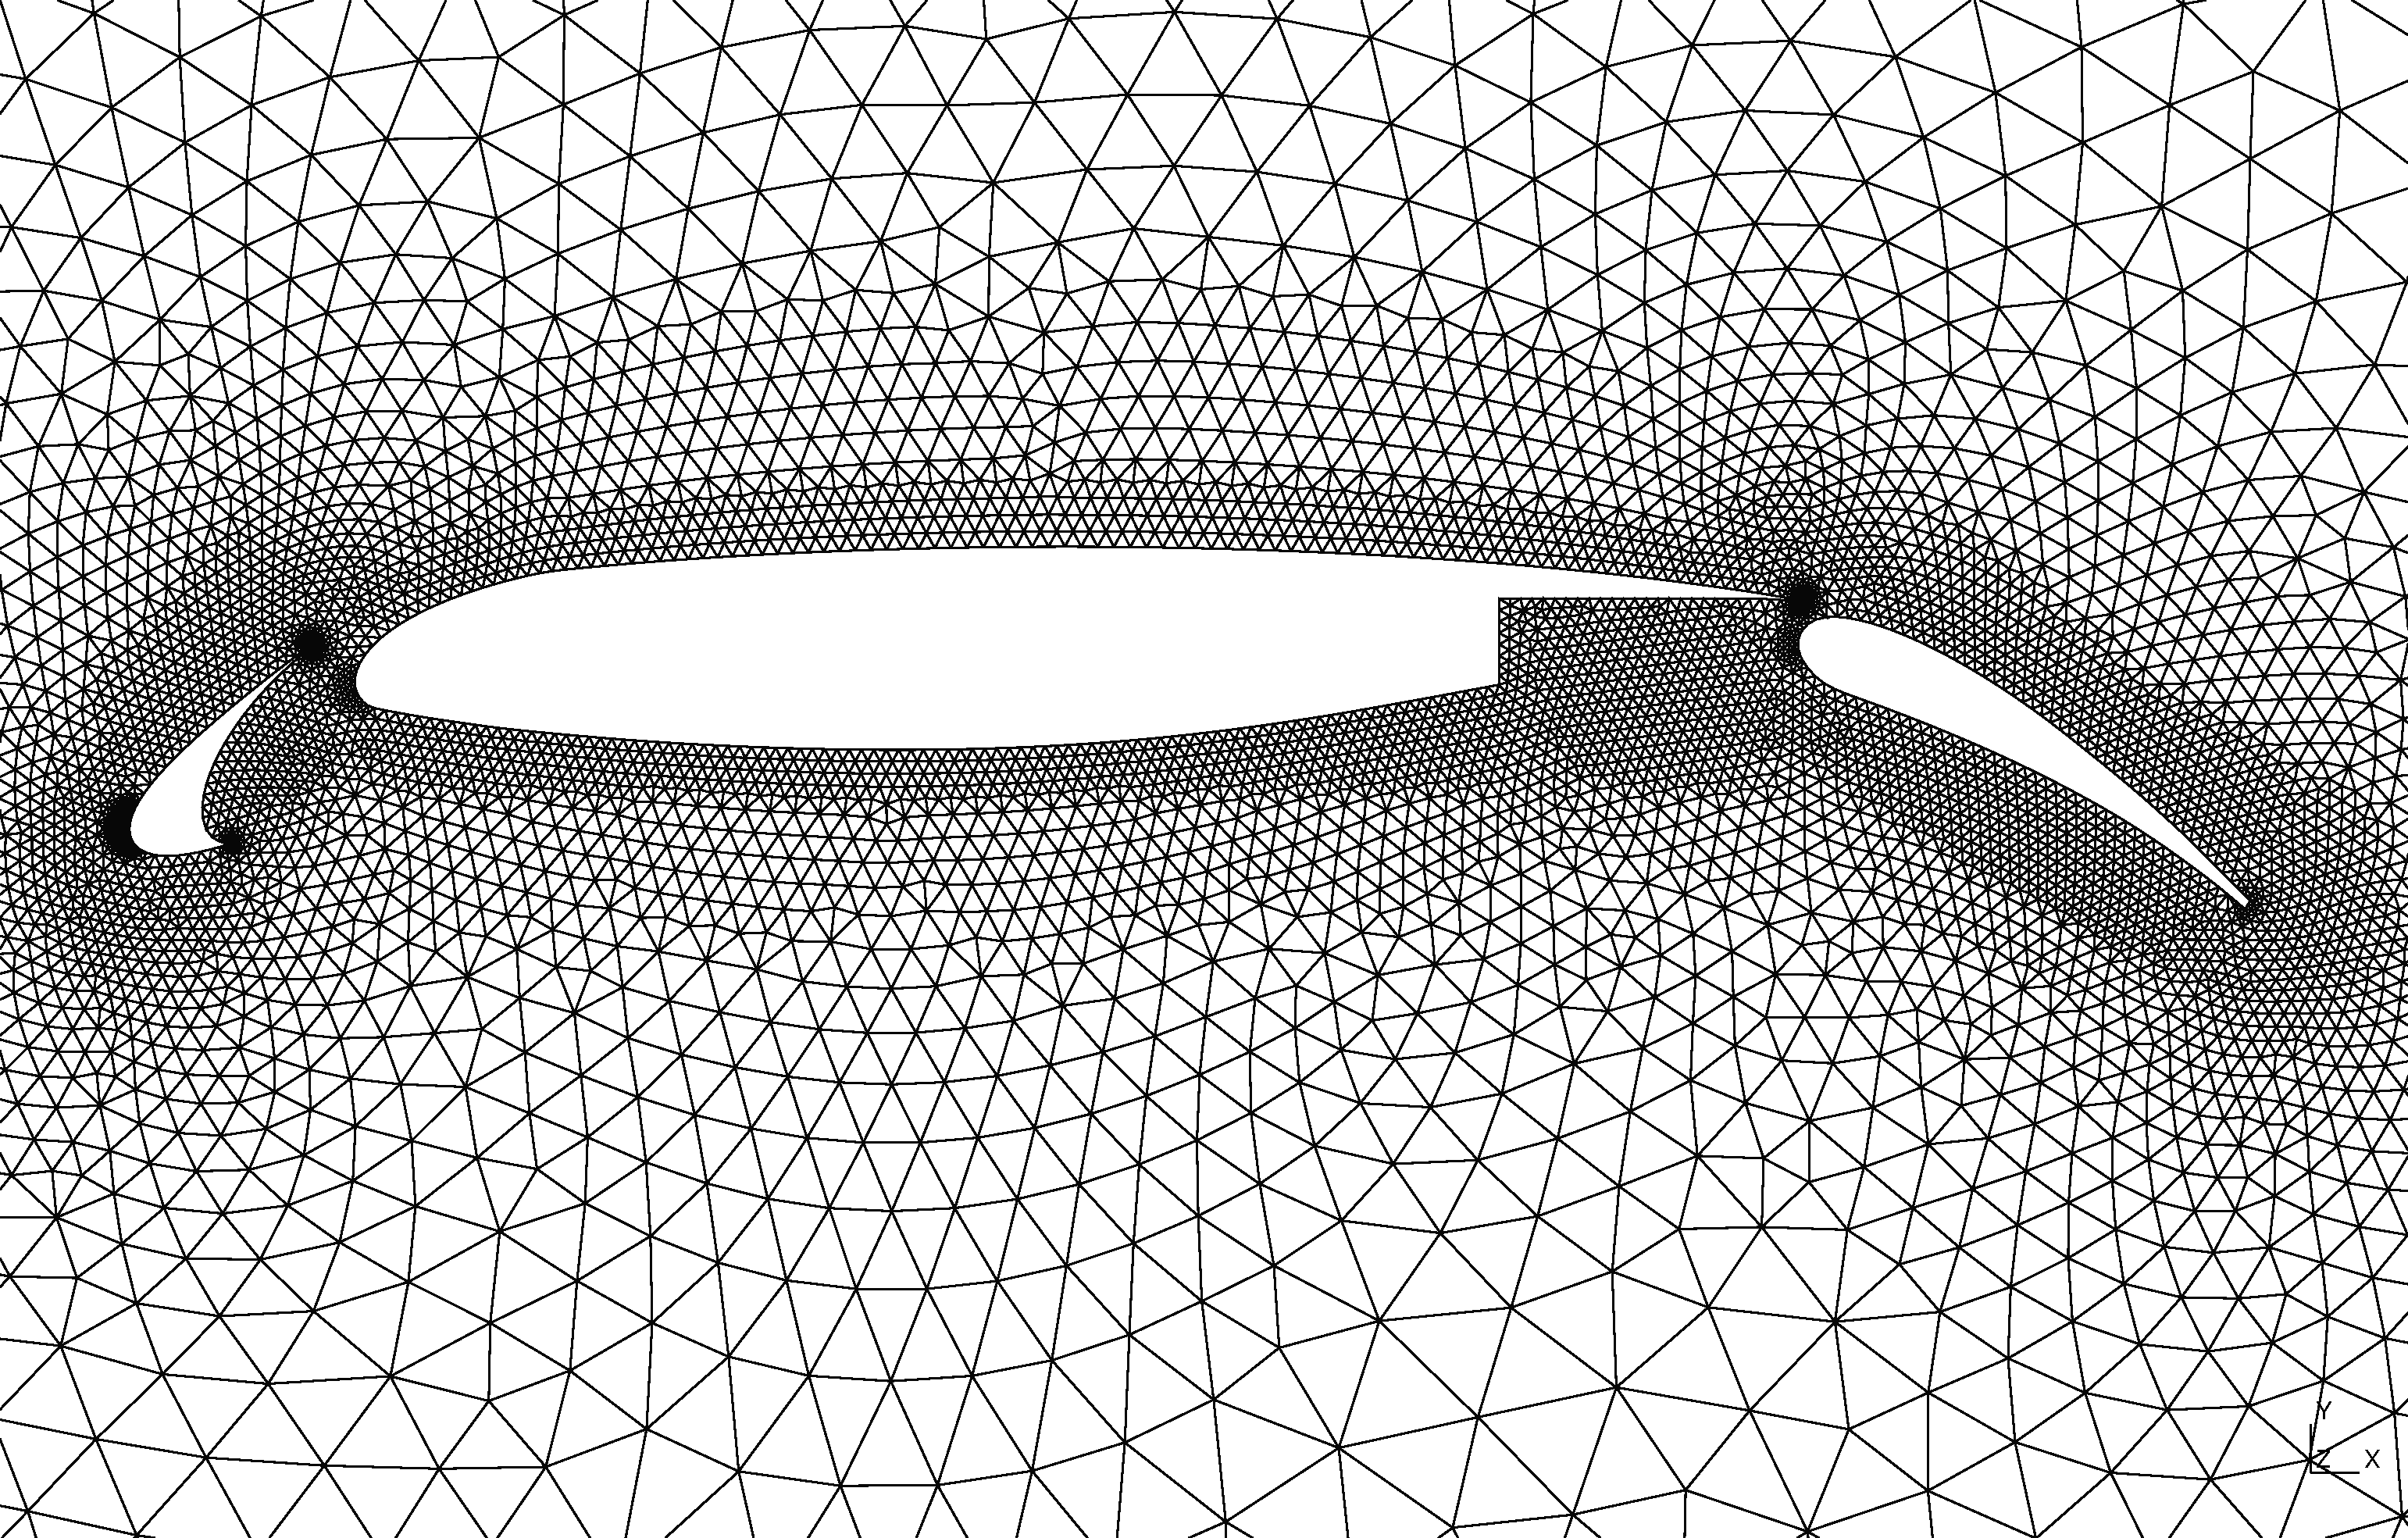
\includegraphics[scale=0.25]{3comp-inviscid}
  	\caption{Original mesh for inviscid flow around 3-component airfoil}
  	\label{fig:wing-inviscid}
\end{figure}

In figure \ref{fig:wing-inviscid-farhat}, we show the result of the torsion spring method of Farhat et. al. \cite{mm:torsionsprings}. We see that the result for such a large deformation is not acceptable; it is evident that there are invalid cells. It is interesting to note that cells near the trailing edge of the middle wing do not suffer much degradation, but cells somewhat farther away become invalid. Cells near the trailing edge of the flap also suffer large distortions.

\begin{figure}
	\centering
	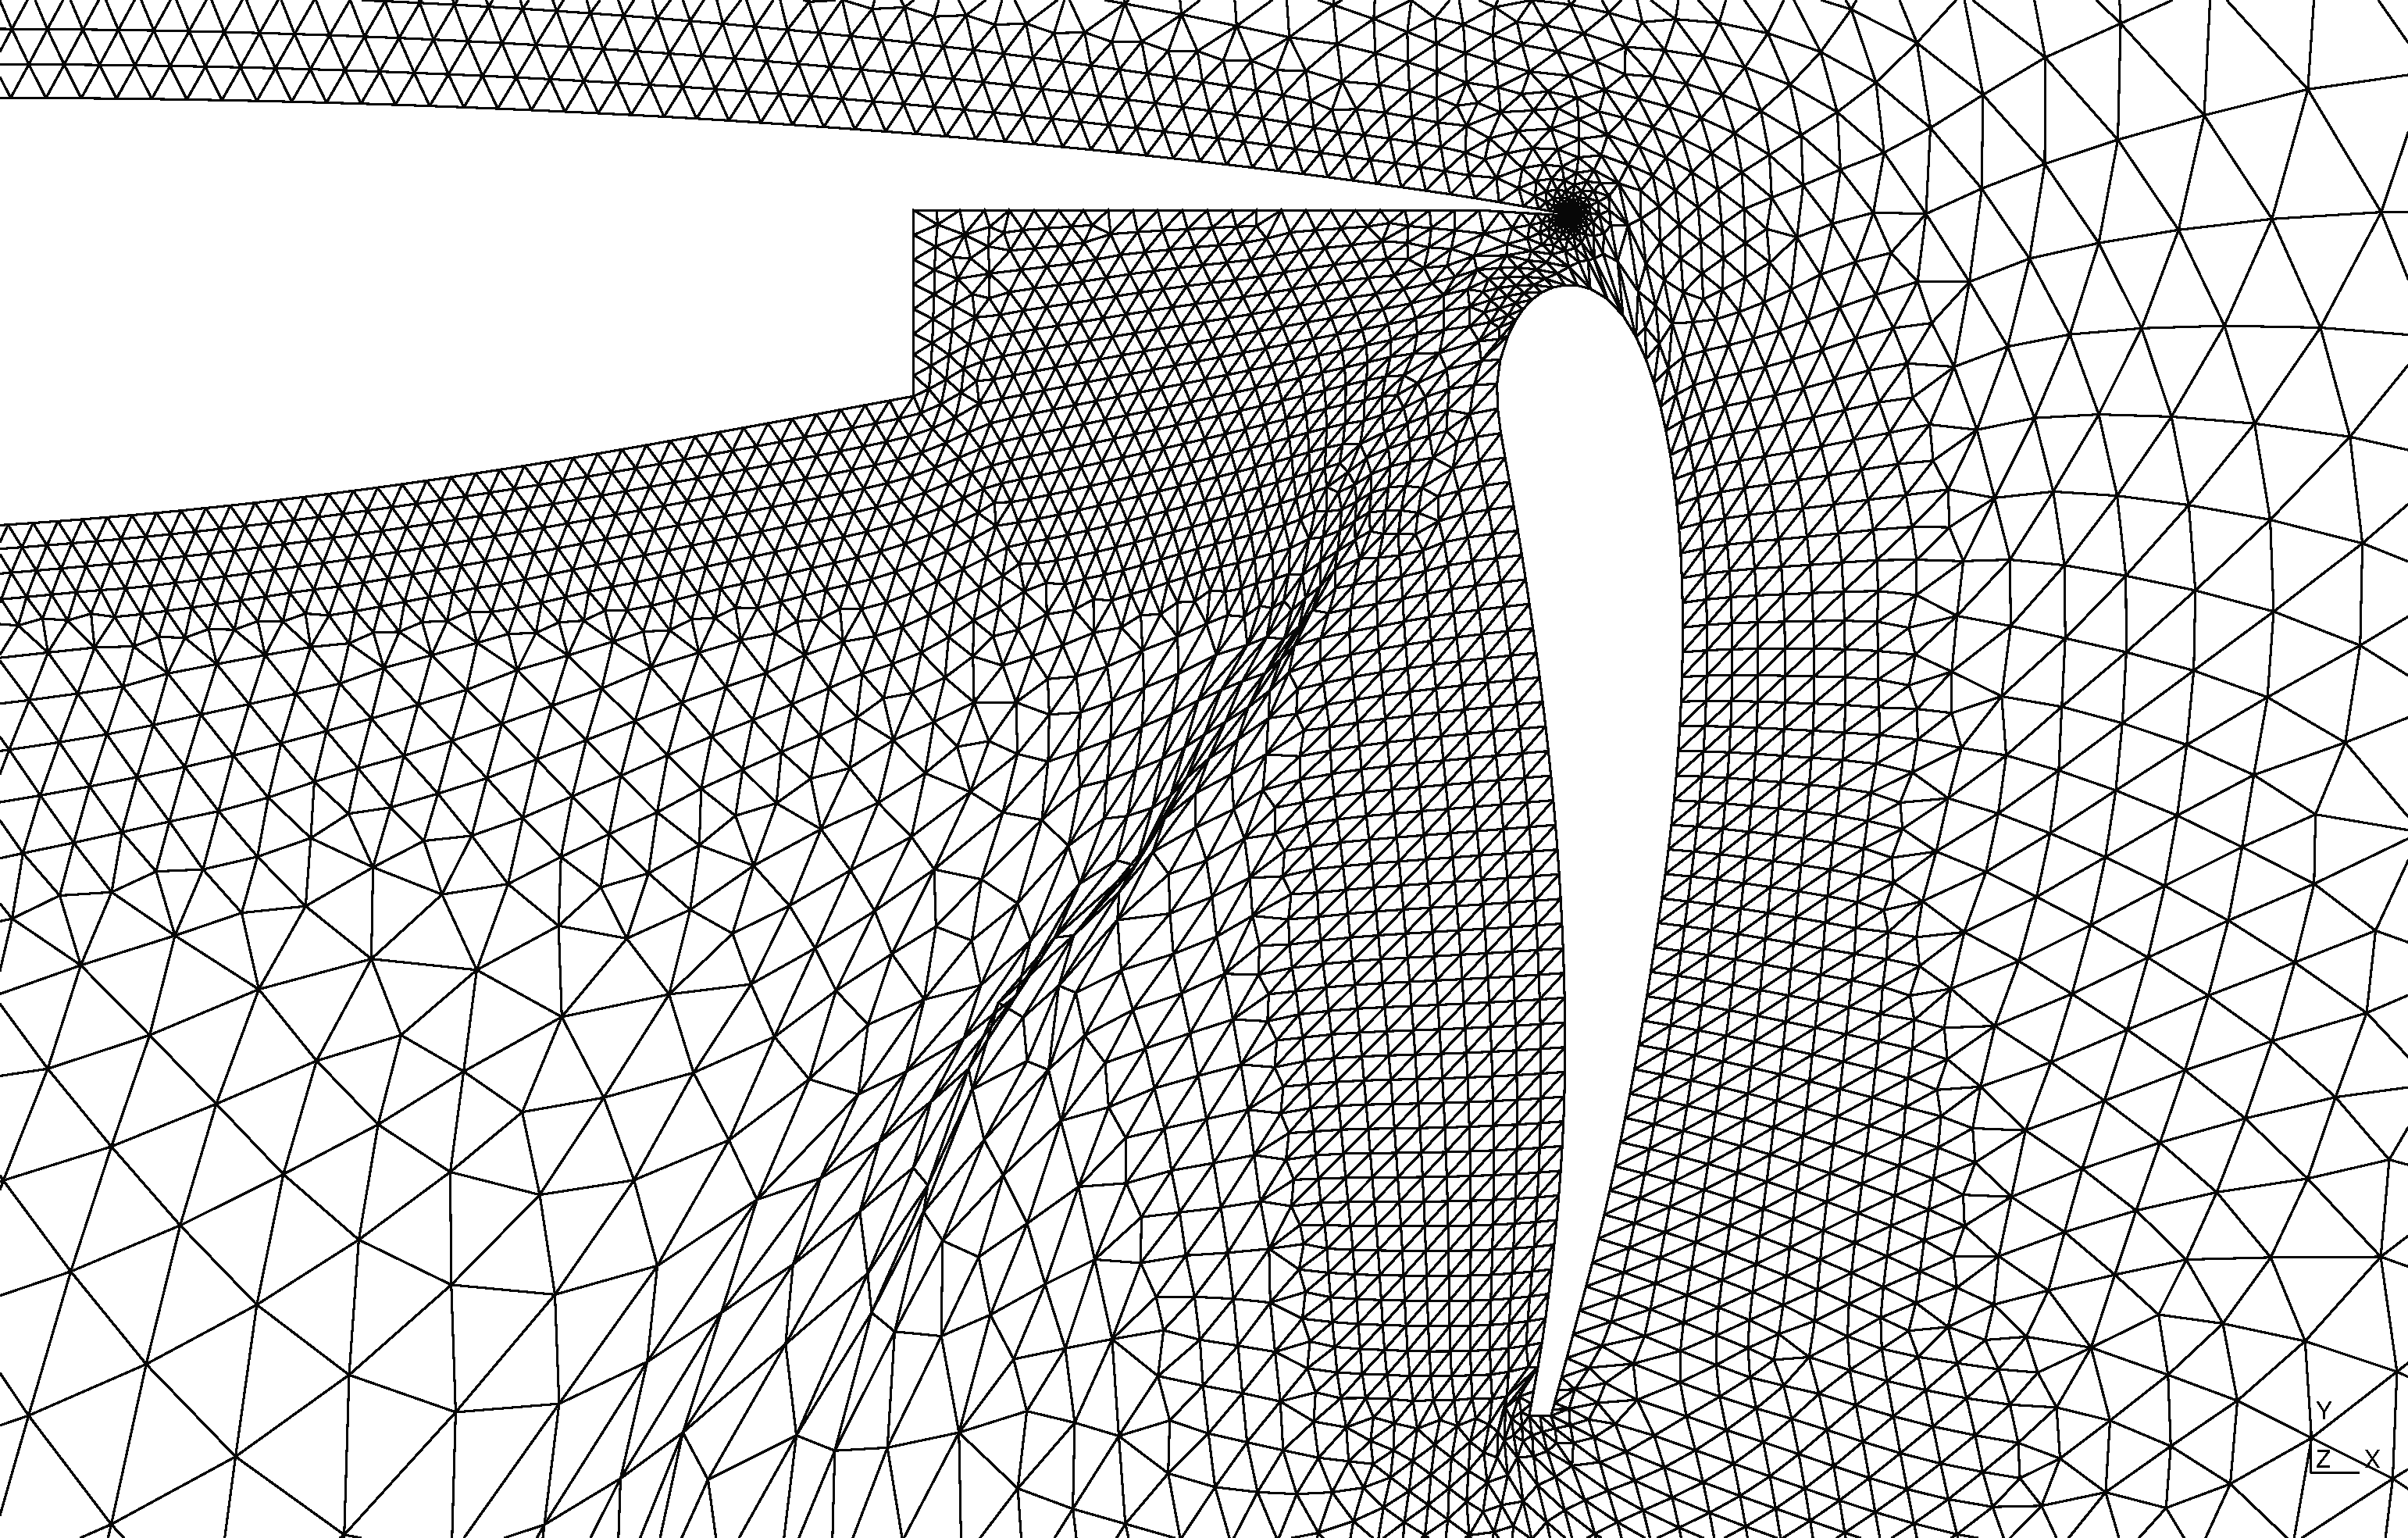
\includegraphics[scale=0.25]{wing60-farhat}
	\caption{Inviscid 3-component airfoil mesh with 60$^\circ$ rotation of flap by torsion spring method}
	\label{fig:wing-inviscid-farhat}
\end{figure}

Next, results of mesh movement by linear elasticity method are shown in figures \ref{fig:wing-inviscid-linelastp1}, \ref{fig:wing-inviscid-linelastp1-zoomed} and \ref{fig:wing-inviscid-linelastp1-zoomed2}. The mesh is valid; however, it suffers from nearly-degenerate cells near the trailing edge of the flap \ref{fig:wing-inviscid-linelastp1-zoomed2}. This could seriously impact the performance, accuracy and even stability of flow solvers using this mesh. In figure \ref{fig:wing-inviscid-linelastp1-zoomed}, we  see that the quality of cells is better than near the trailing edge, but not very good.

\begin{figure}
	\centering
	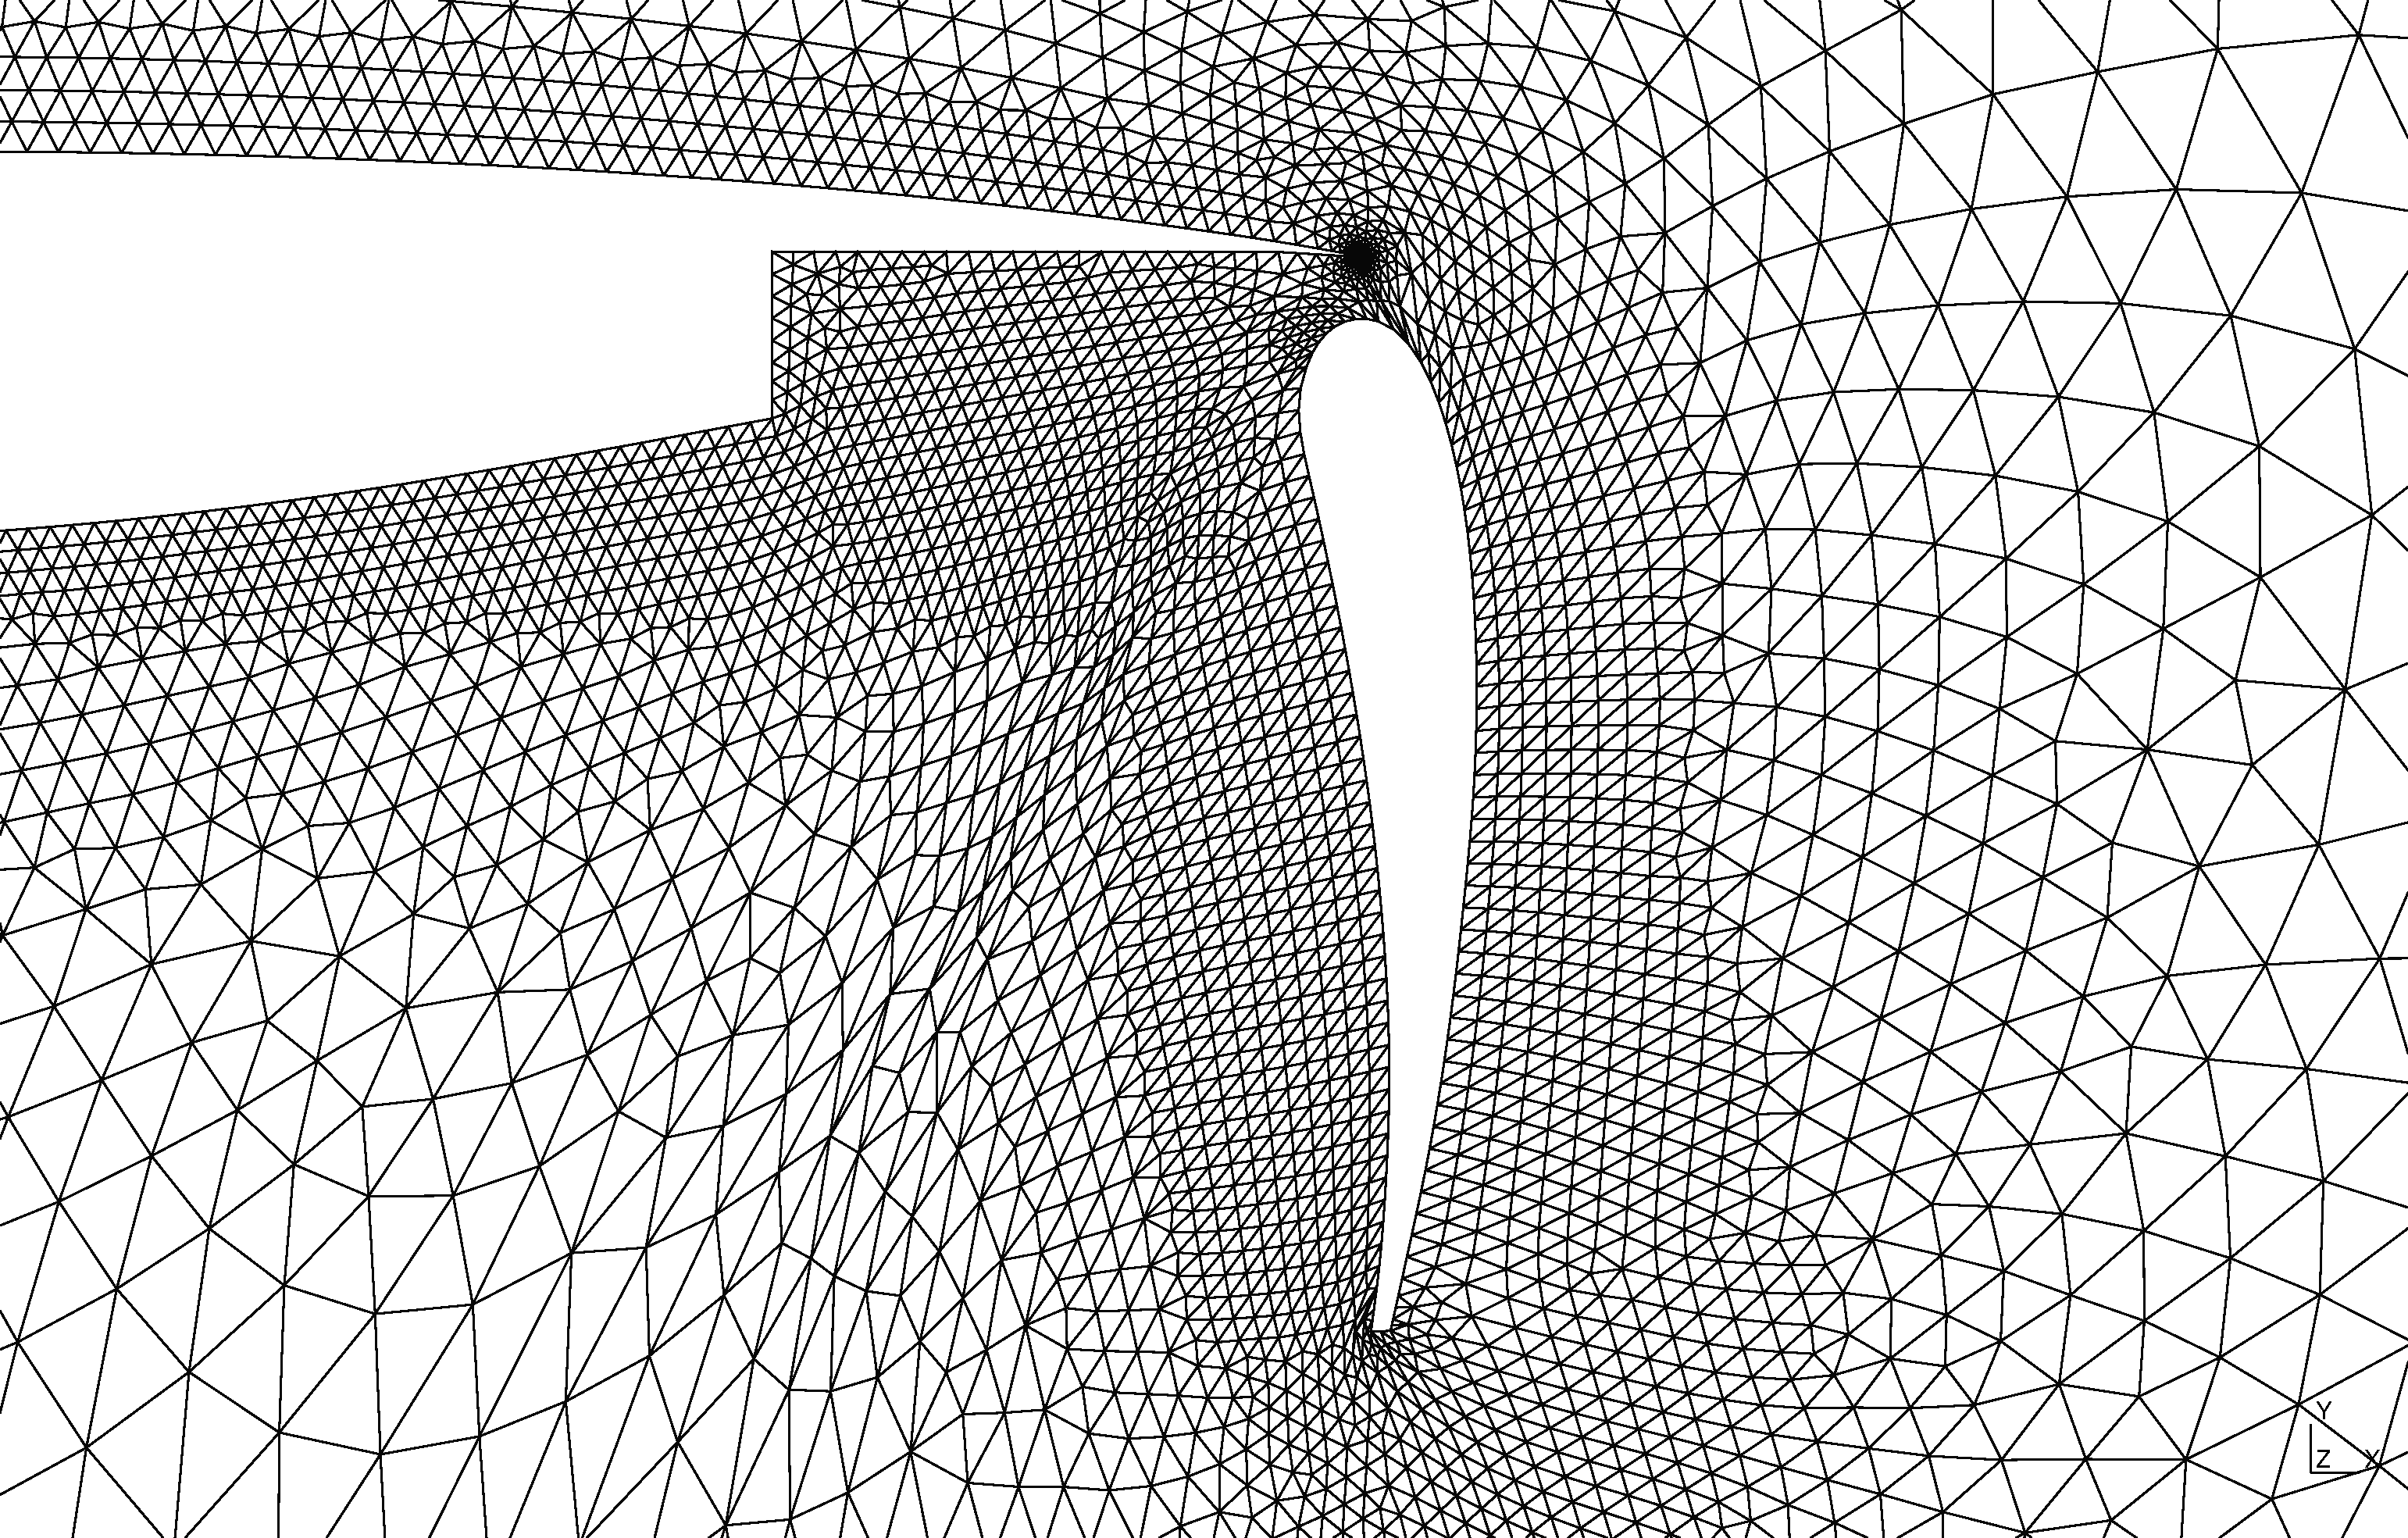
\includegraphics[scale=0.25]{wing60-linelastp1}
	\caption{Inviscid 3-component airfoil mesh with 60$^\circ$ rotation of flap by linear elasticity method}
	\label{fig:wing-inviscid-linelastp1}
\end{figure}
\begin{figure}
	\centering
	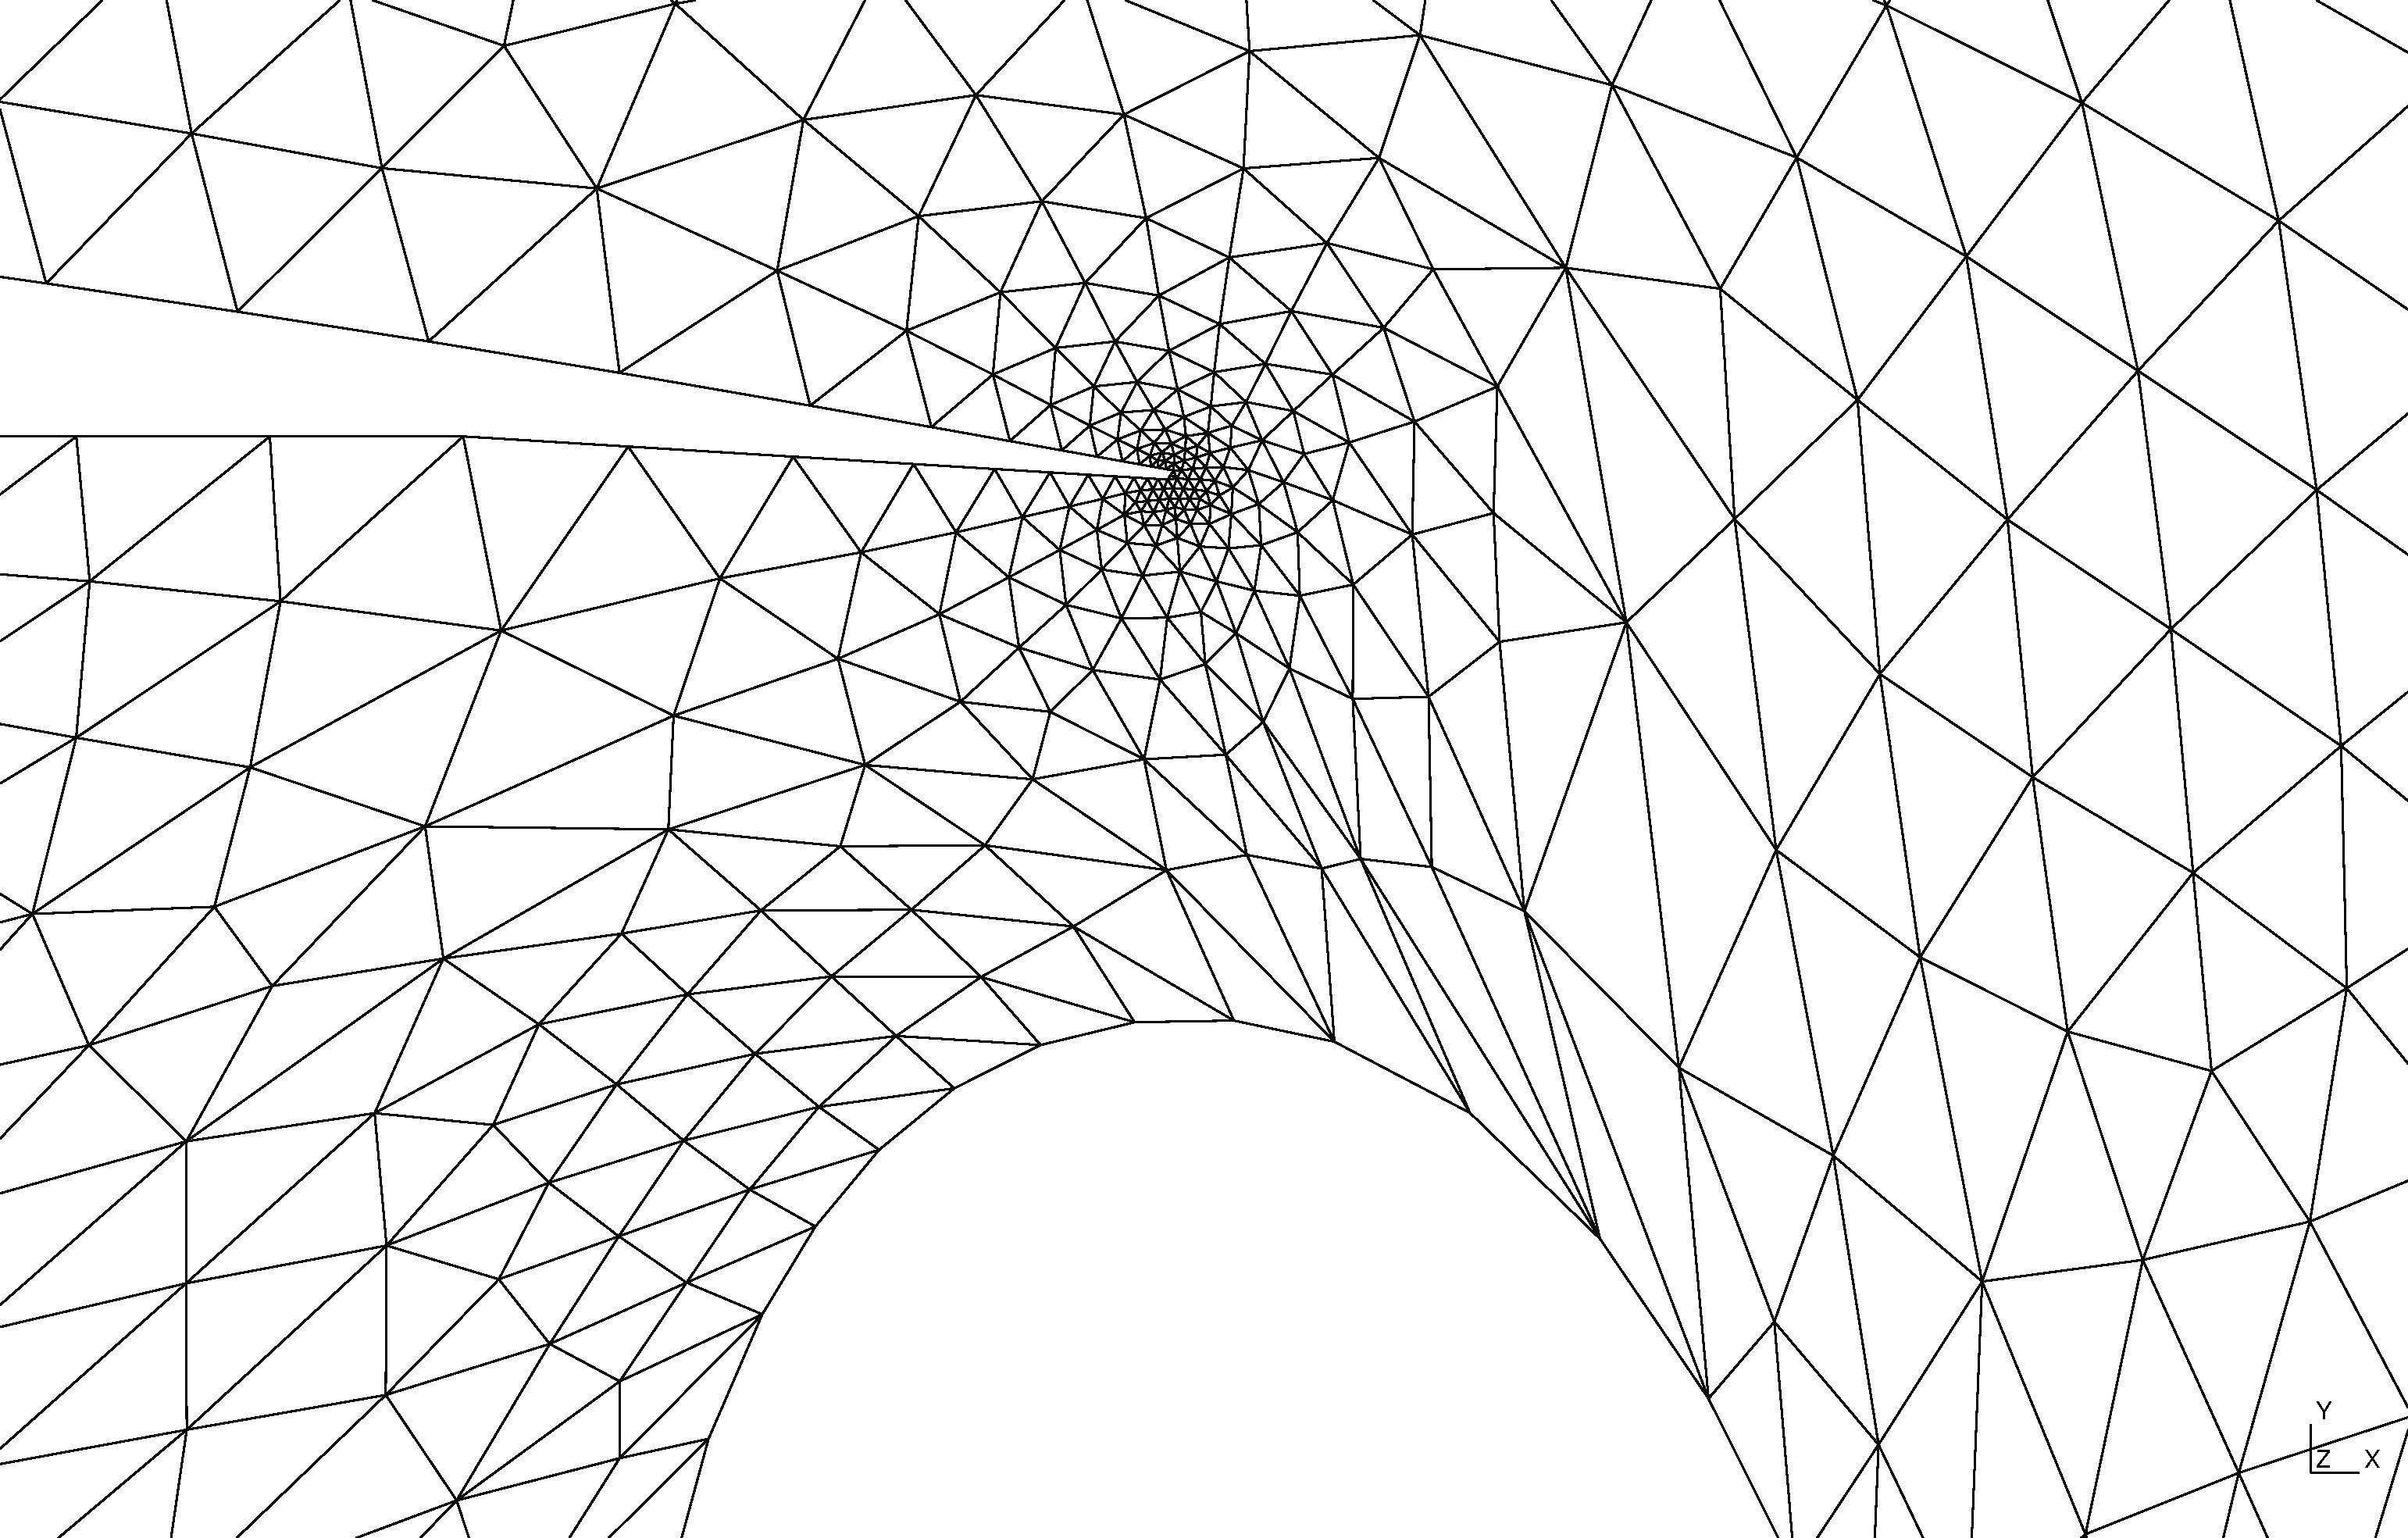
\includegraphics[scale=0.25]{wing60-linelastp1_zoomed}
	\caption{Inviscid 3-component airfoil mesh with 60$^\circ$ rotation of flap by linear elasticity method; zoomed to where the flap meets the wing}
	\label{fig:wing-inviscid-linelastp1-zoomed}
\end{figure}
\begin{figure}
	\centering
	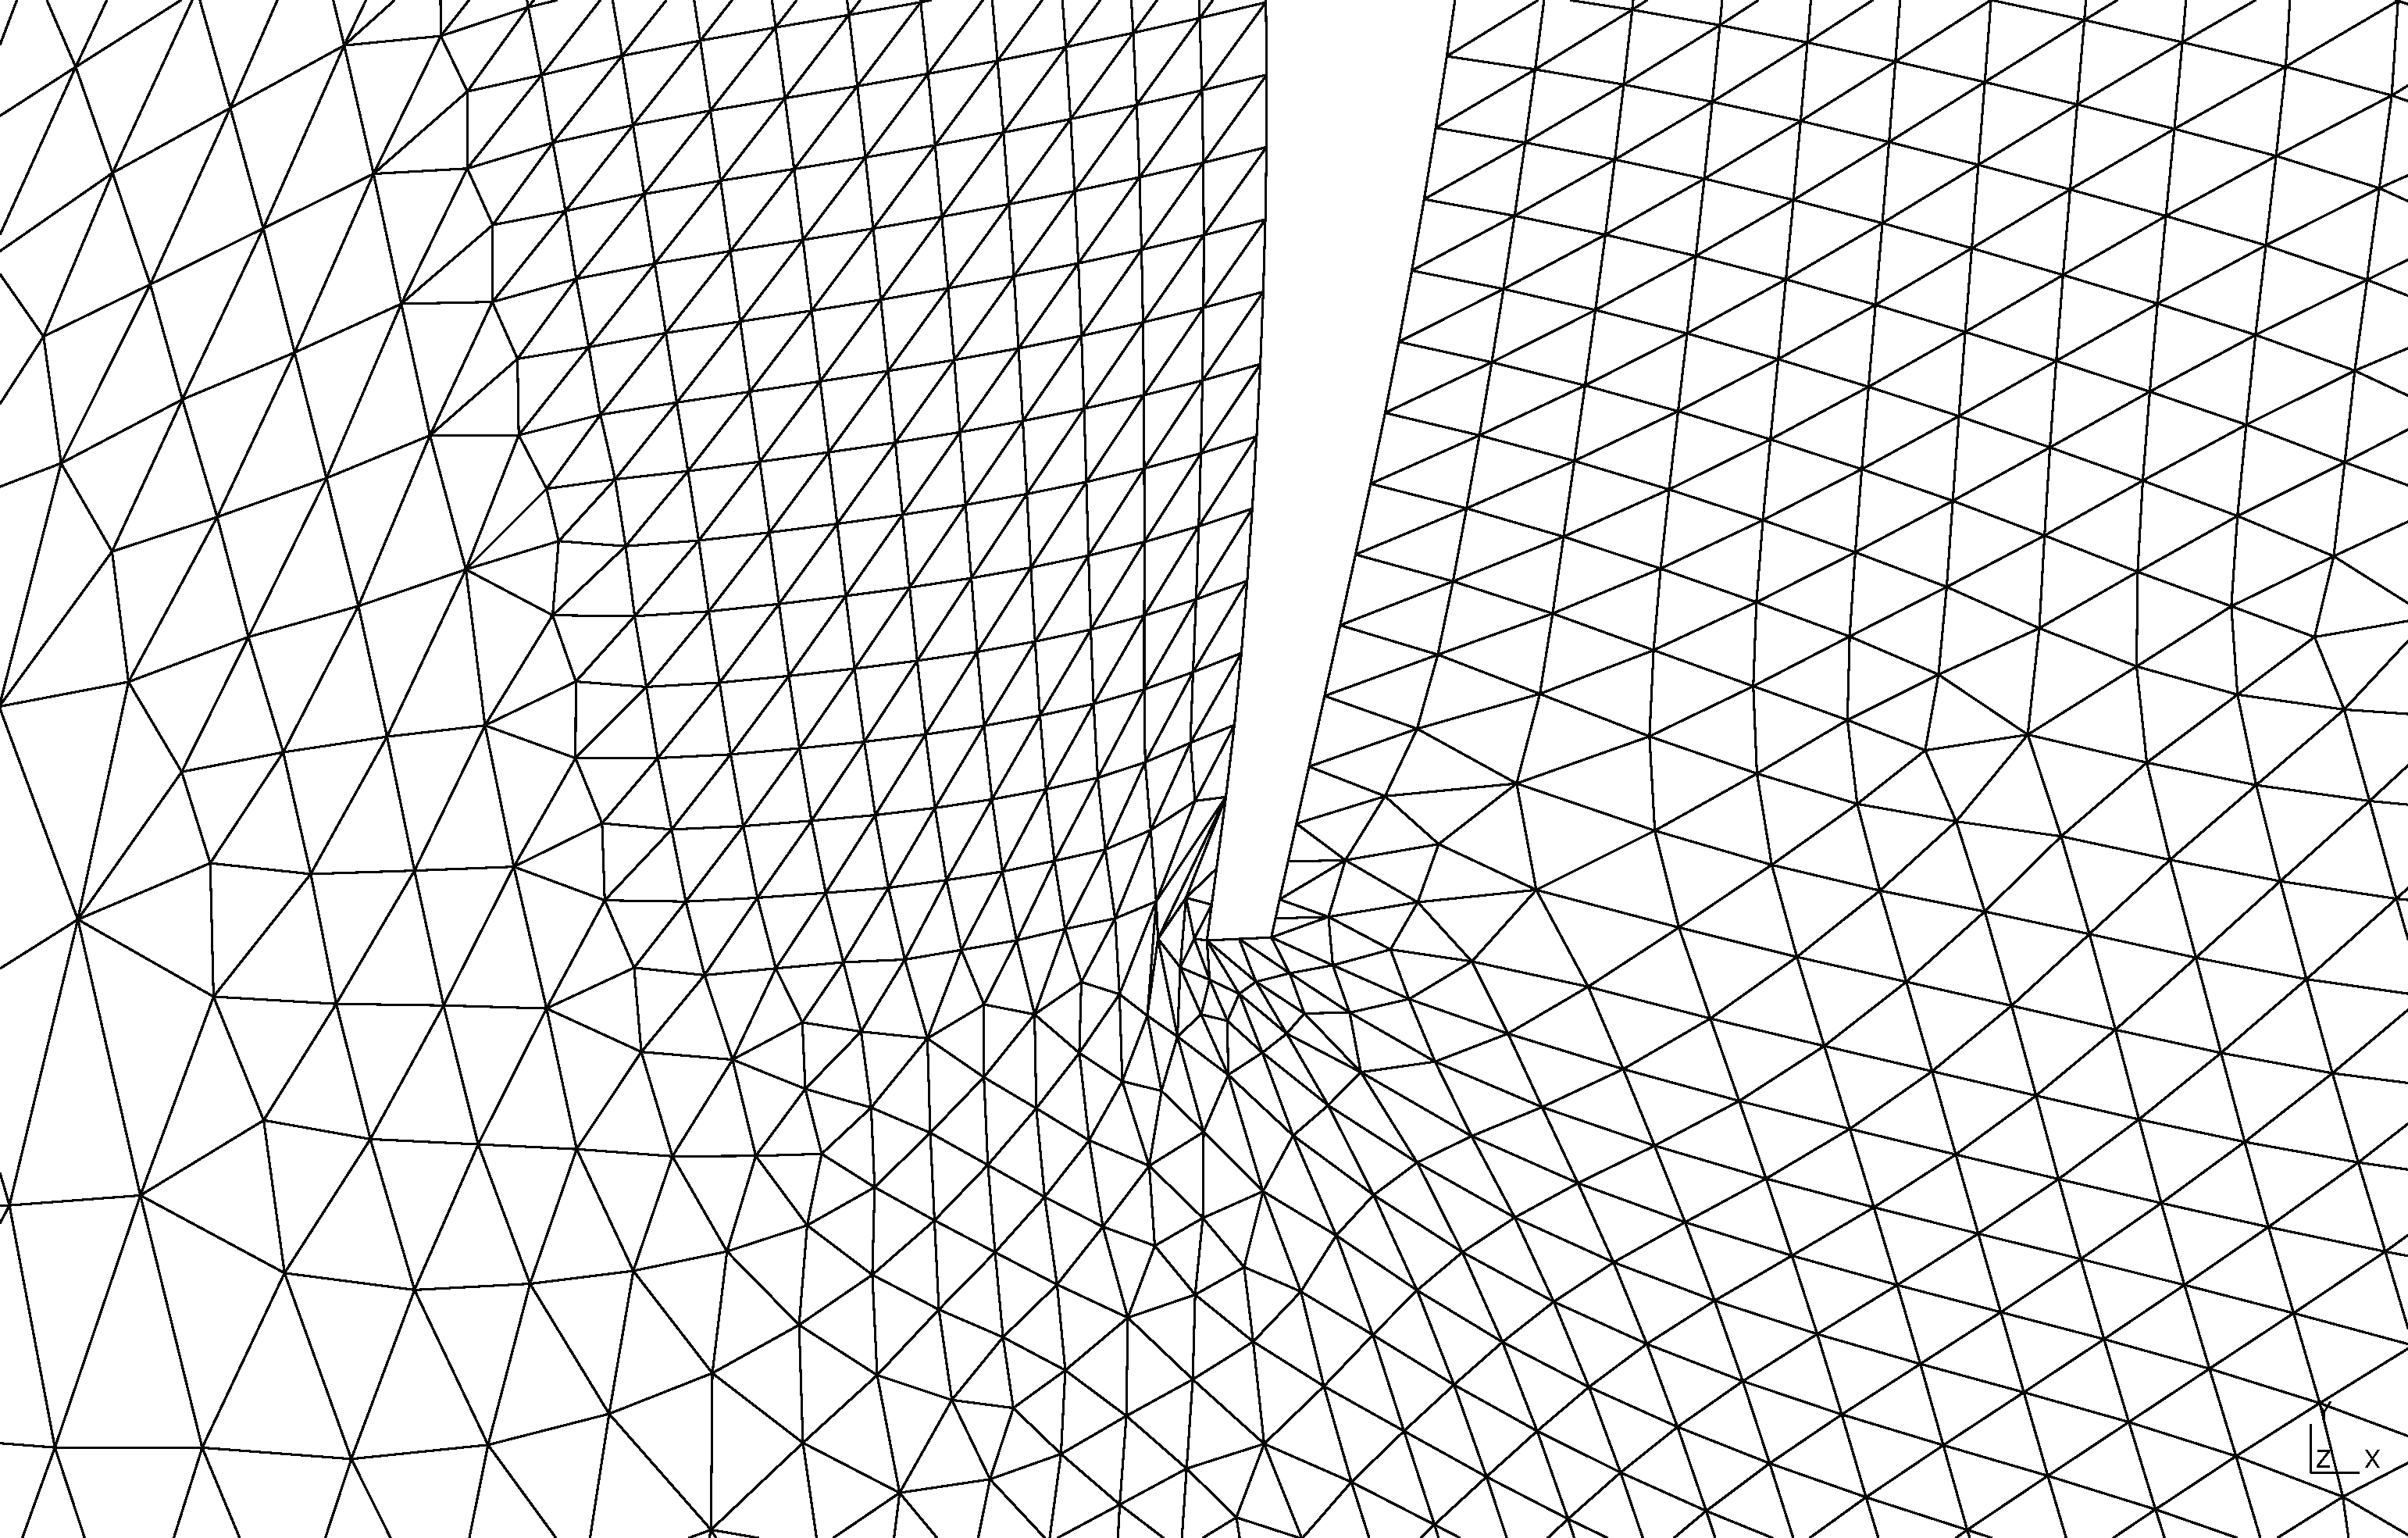
\includegraphics[scale=0.25]{wing60-linelastp1_zoomed2}
	\caption{Inviscid 3-component airfoil mesh with 60$^\circ$ rotation of flap by linear elasticity method, zoomed to the trailing edge of the flap}
	\label{fig:wing-inviscid-linelastp1-zoomed2}
\end{figure}

In figures \ref{fig:wing-inviscid-dg-ms} and \ref{fig:wing-inviscid-dg-ms-zoomed}, we present results with the Delaunay graph mapping (DGM) method. We see that cell quality is severly degraded near the interface between trailing edge of the wing and the flap. The quality of the cells near the trailing edge of the flap is better than the linear elasticity case, however. We remark here that DGM is computationally the most frugal method out of all the ones presented, as we need to solve only 3x3 linear systems after generating a background Delaunay graph, both of which are very fast (sec. \ref{sec:dgm}).

\begin{figure}
	\centering
	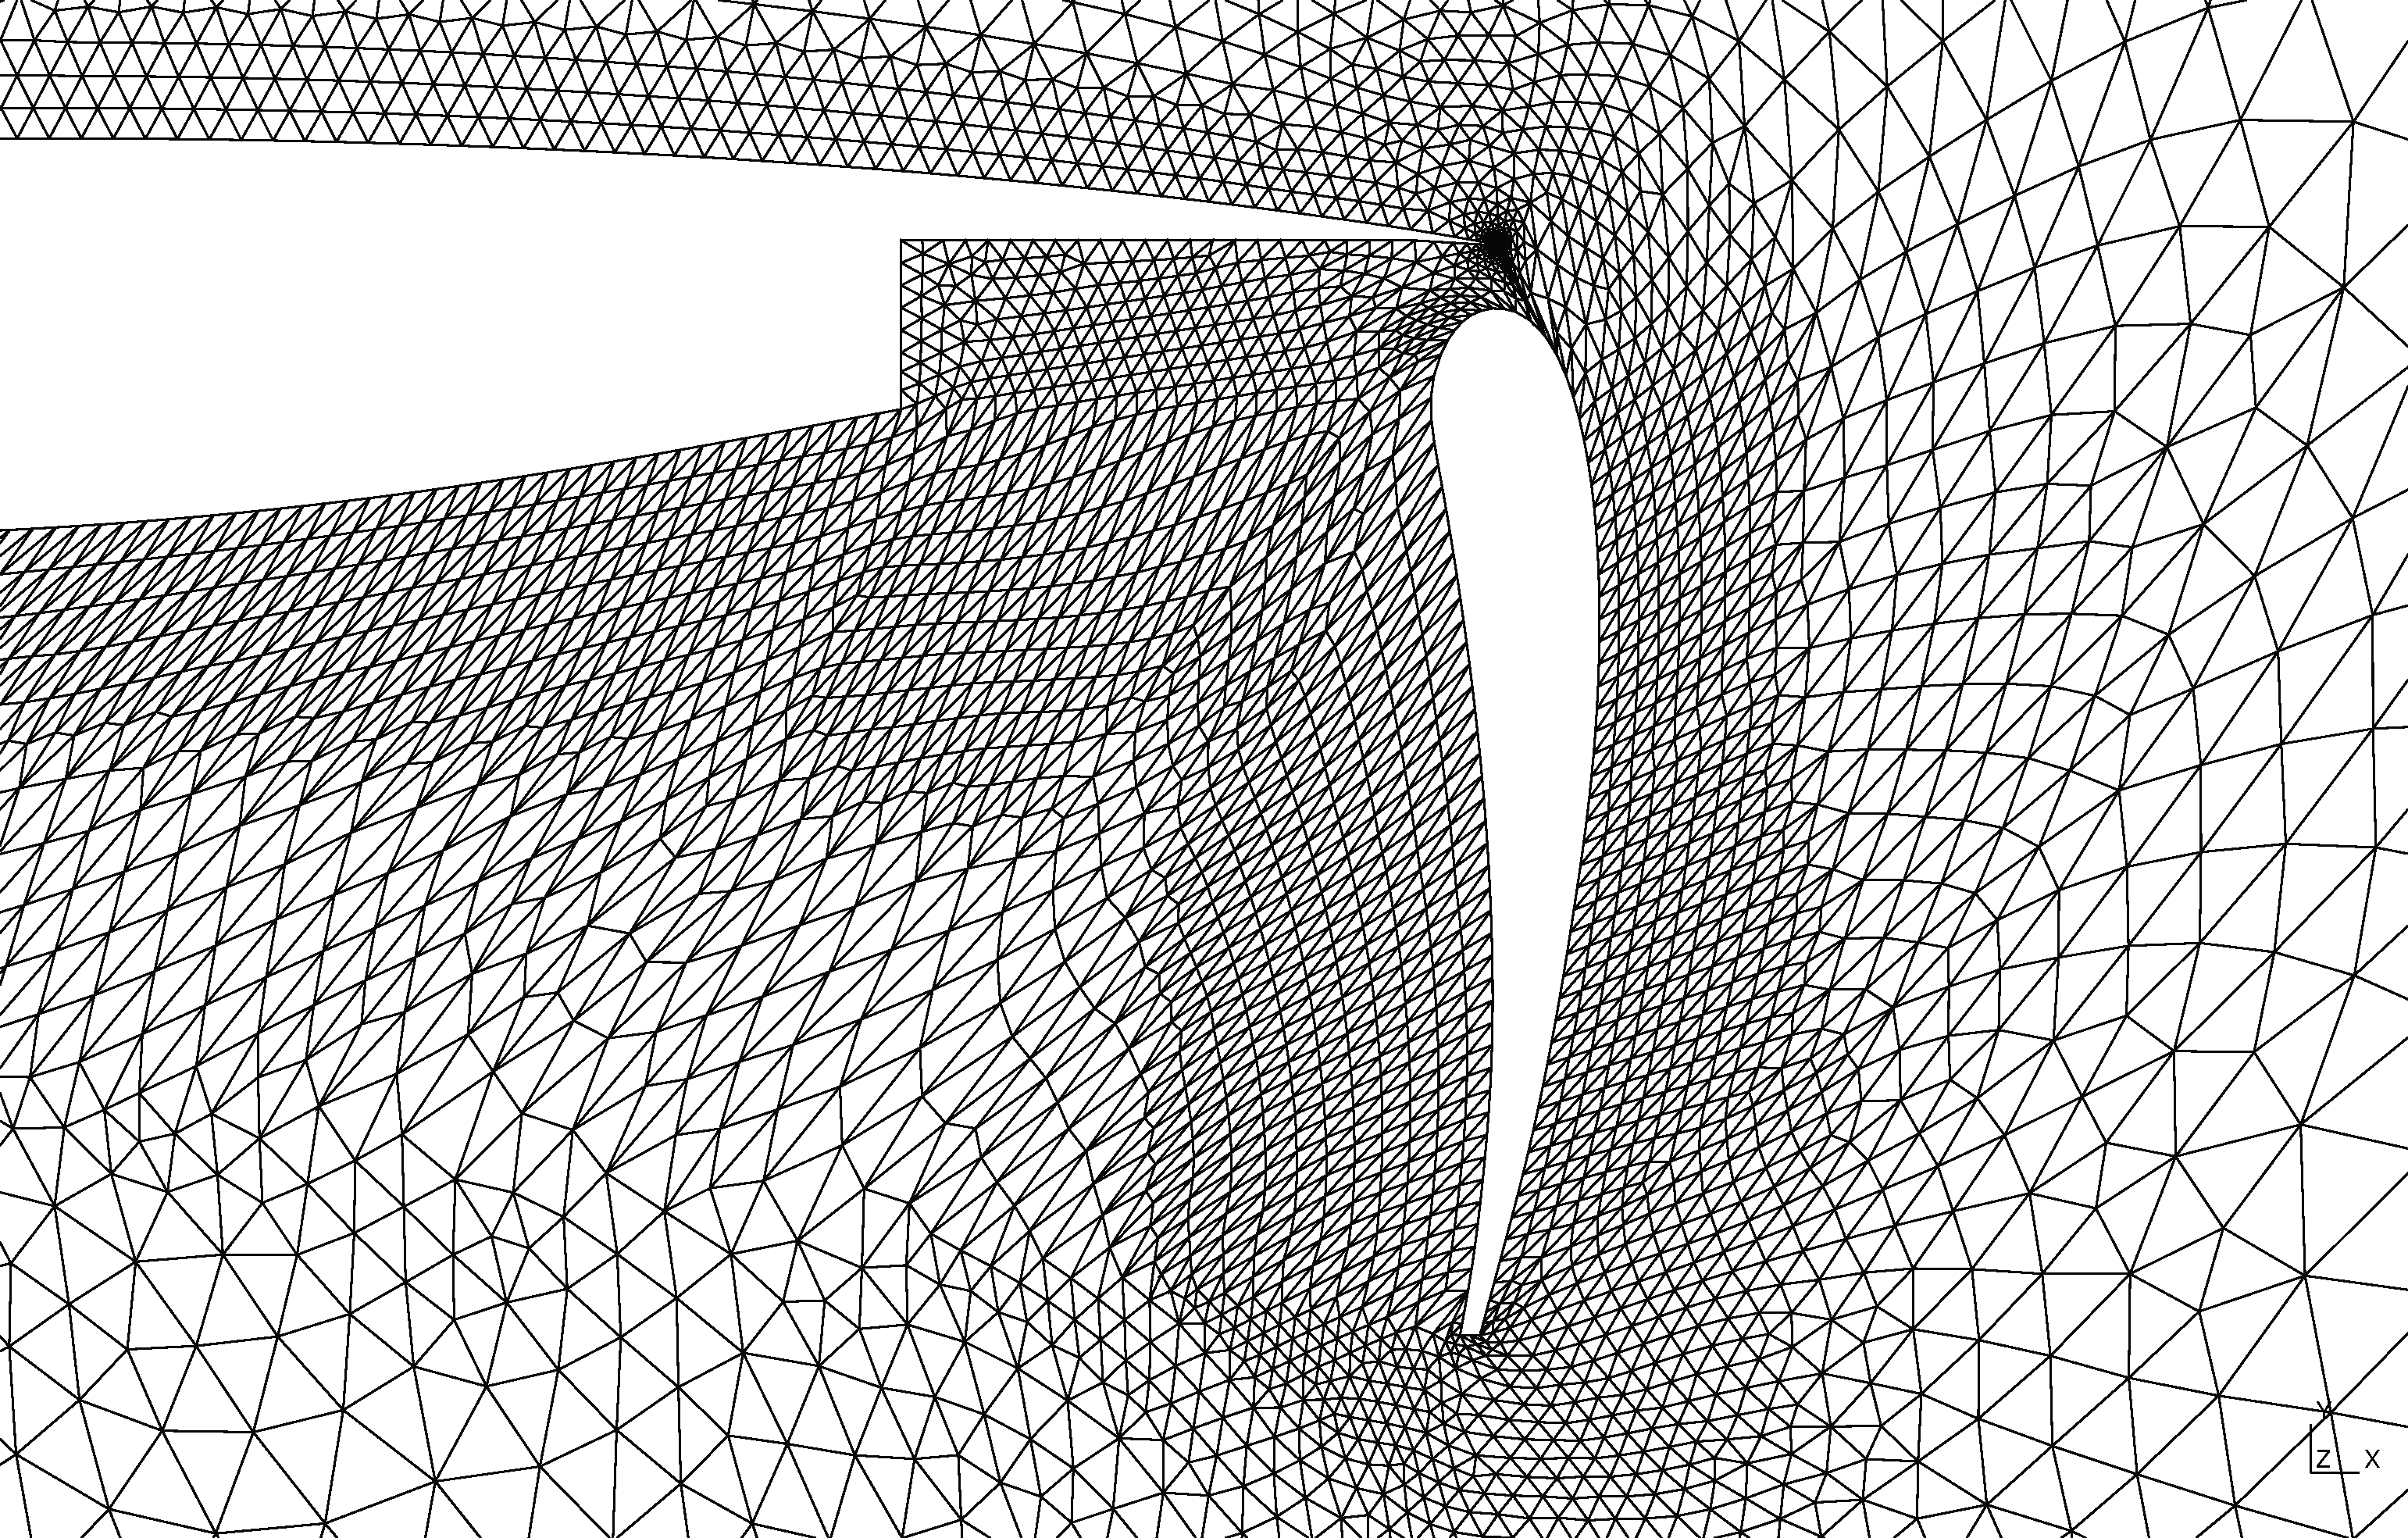
\includegraphics[scale=0.25]{wing60-dg-ms}
	\caption{Inviscid 3-component airfoil mesh with 60$^\circ$ rotation of flap by DGM method}
	\label{fig:wing-inviscid-dg-ms}
\end{figure}
\begin{figure}
	\centering
	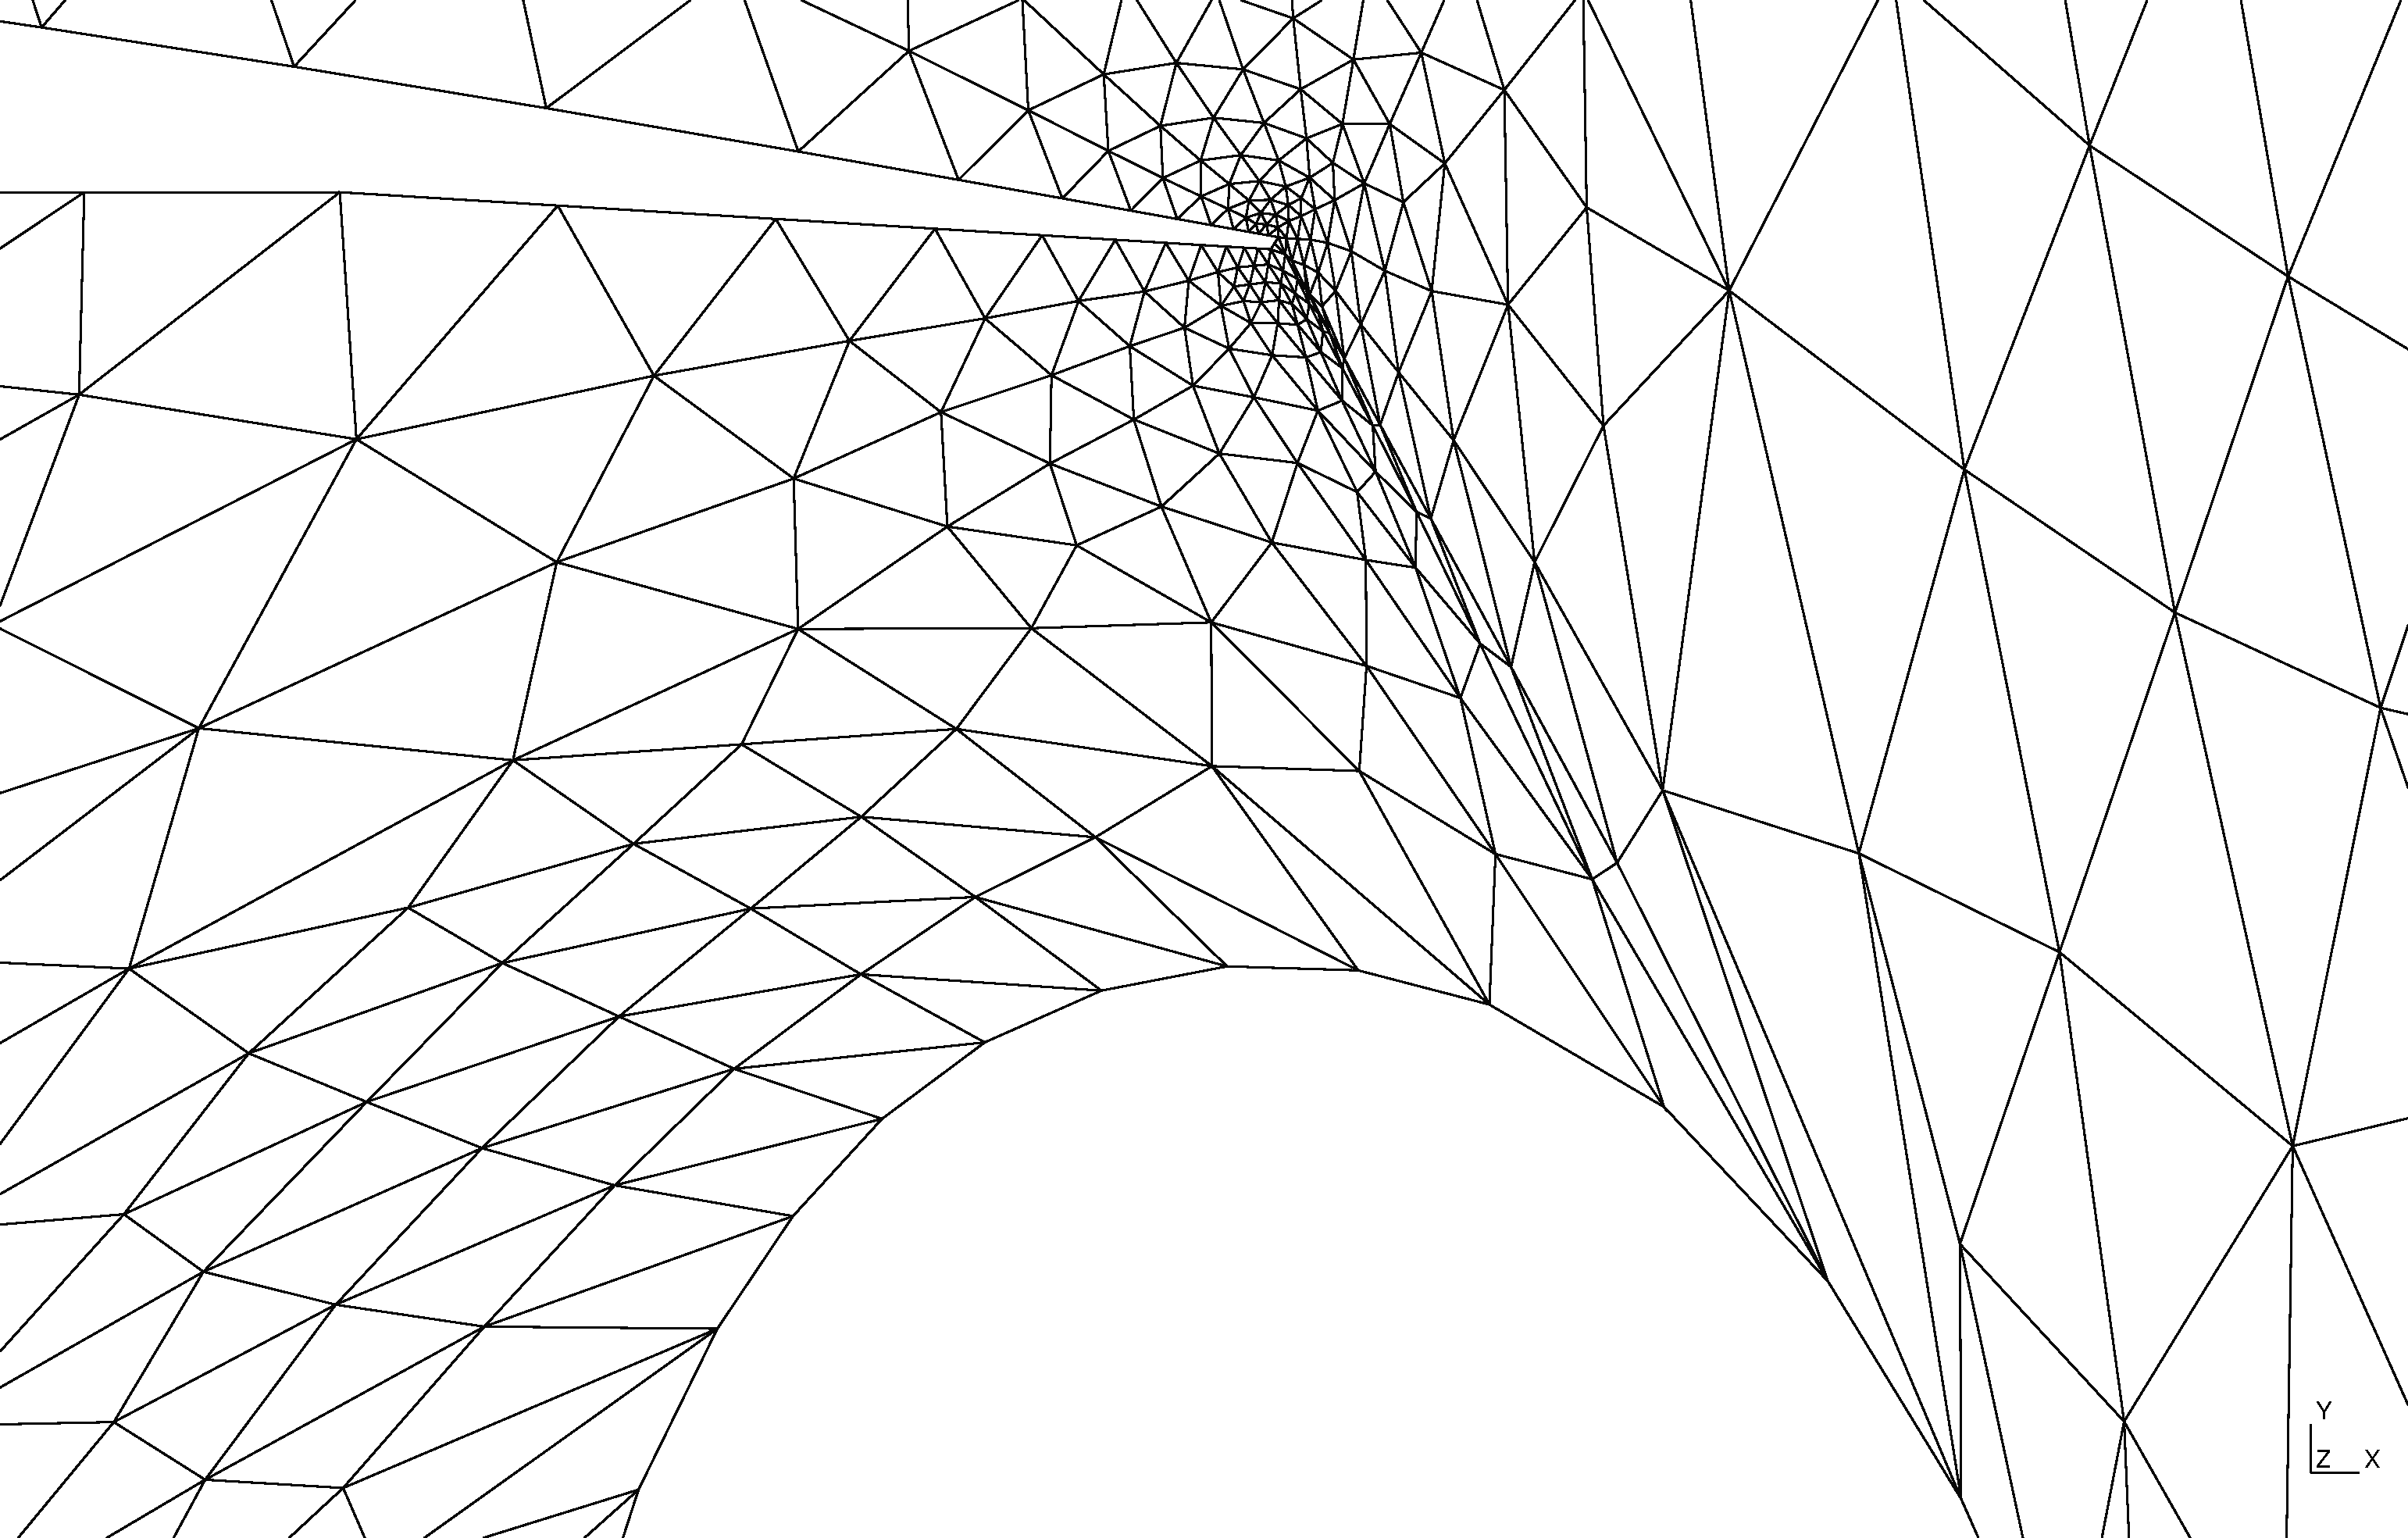
\includegraphics[scale=0.25]{wing60-dg-ms_zoomed}
	\caption{Inviscid 3-component airfoil mesh with 60$^\circ$ rotation of flap by DGM method; zoomed to where the flap meets the wing}
	\label{fig:wing-inviscid-dg-ms-zoomed}
\end{figure}

Finally, we take note of the good qualities of the mesh moved by radial basis function (RBF) interpolation in figures \ref{fig:wing-inviscid-rbf}, \ref{fig:wing-inviscid-rbf-zoomed} and \ref{fig:wing-inviscid-rbf-zoomed2}. We see that mesh quality is not lost to a  great extent anywhere. The support radius is 15.0 units (for reference, the chord length of the wing is approximately 18.3) and the entire movement is carried out in 3 steps.

\begin{figure}
	\centering
	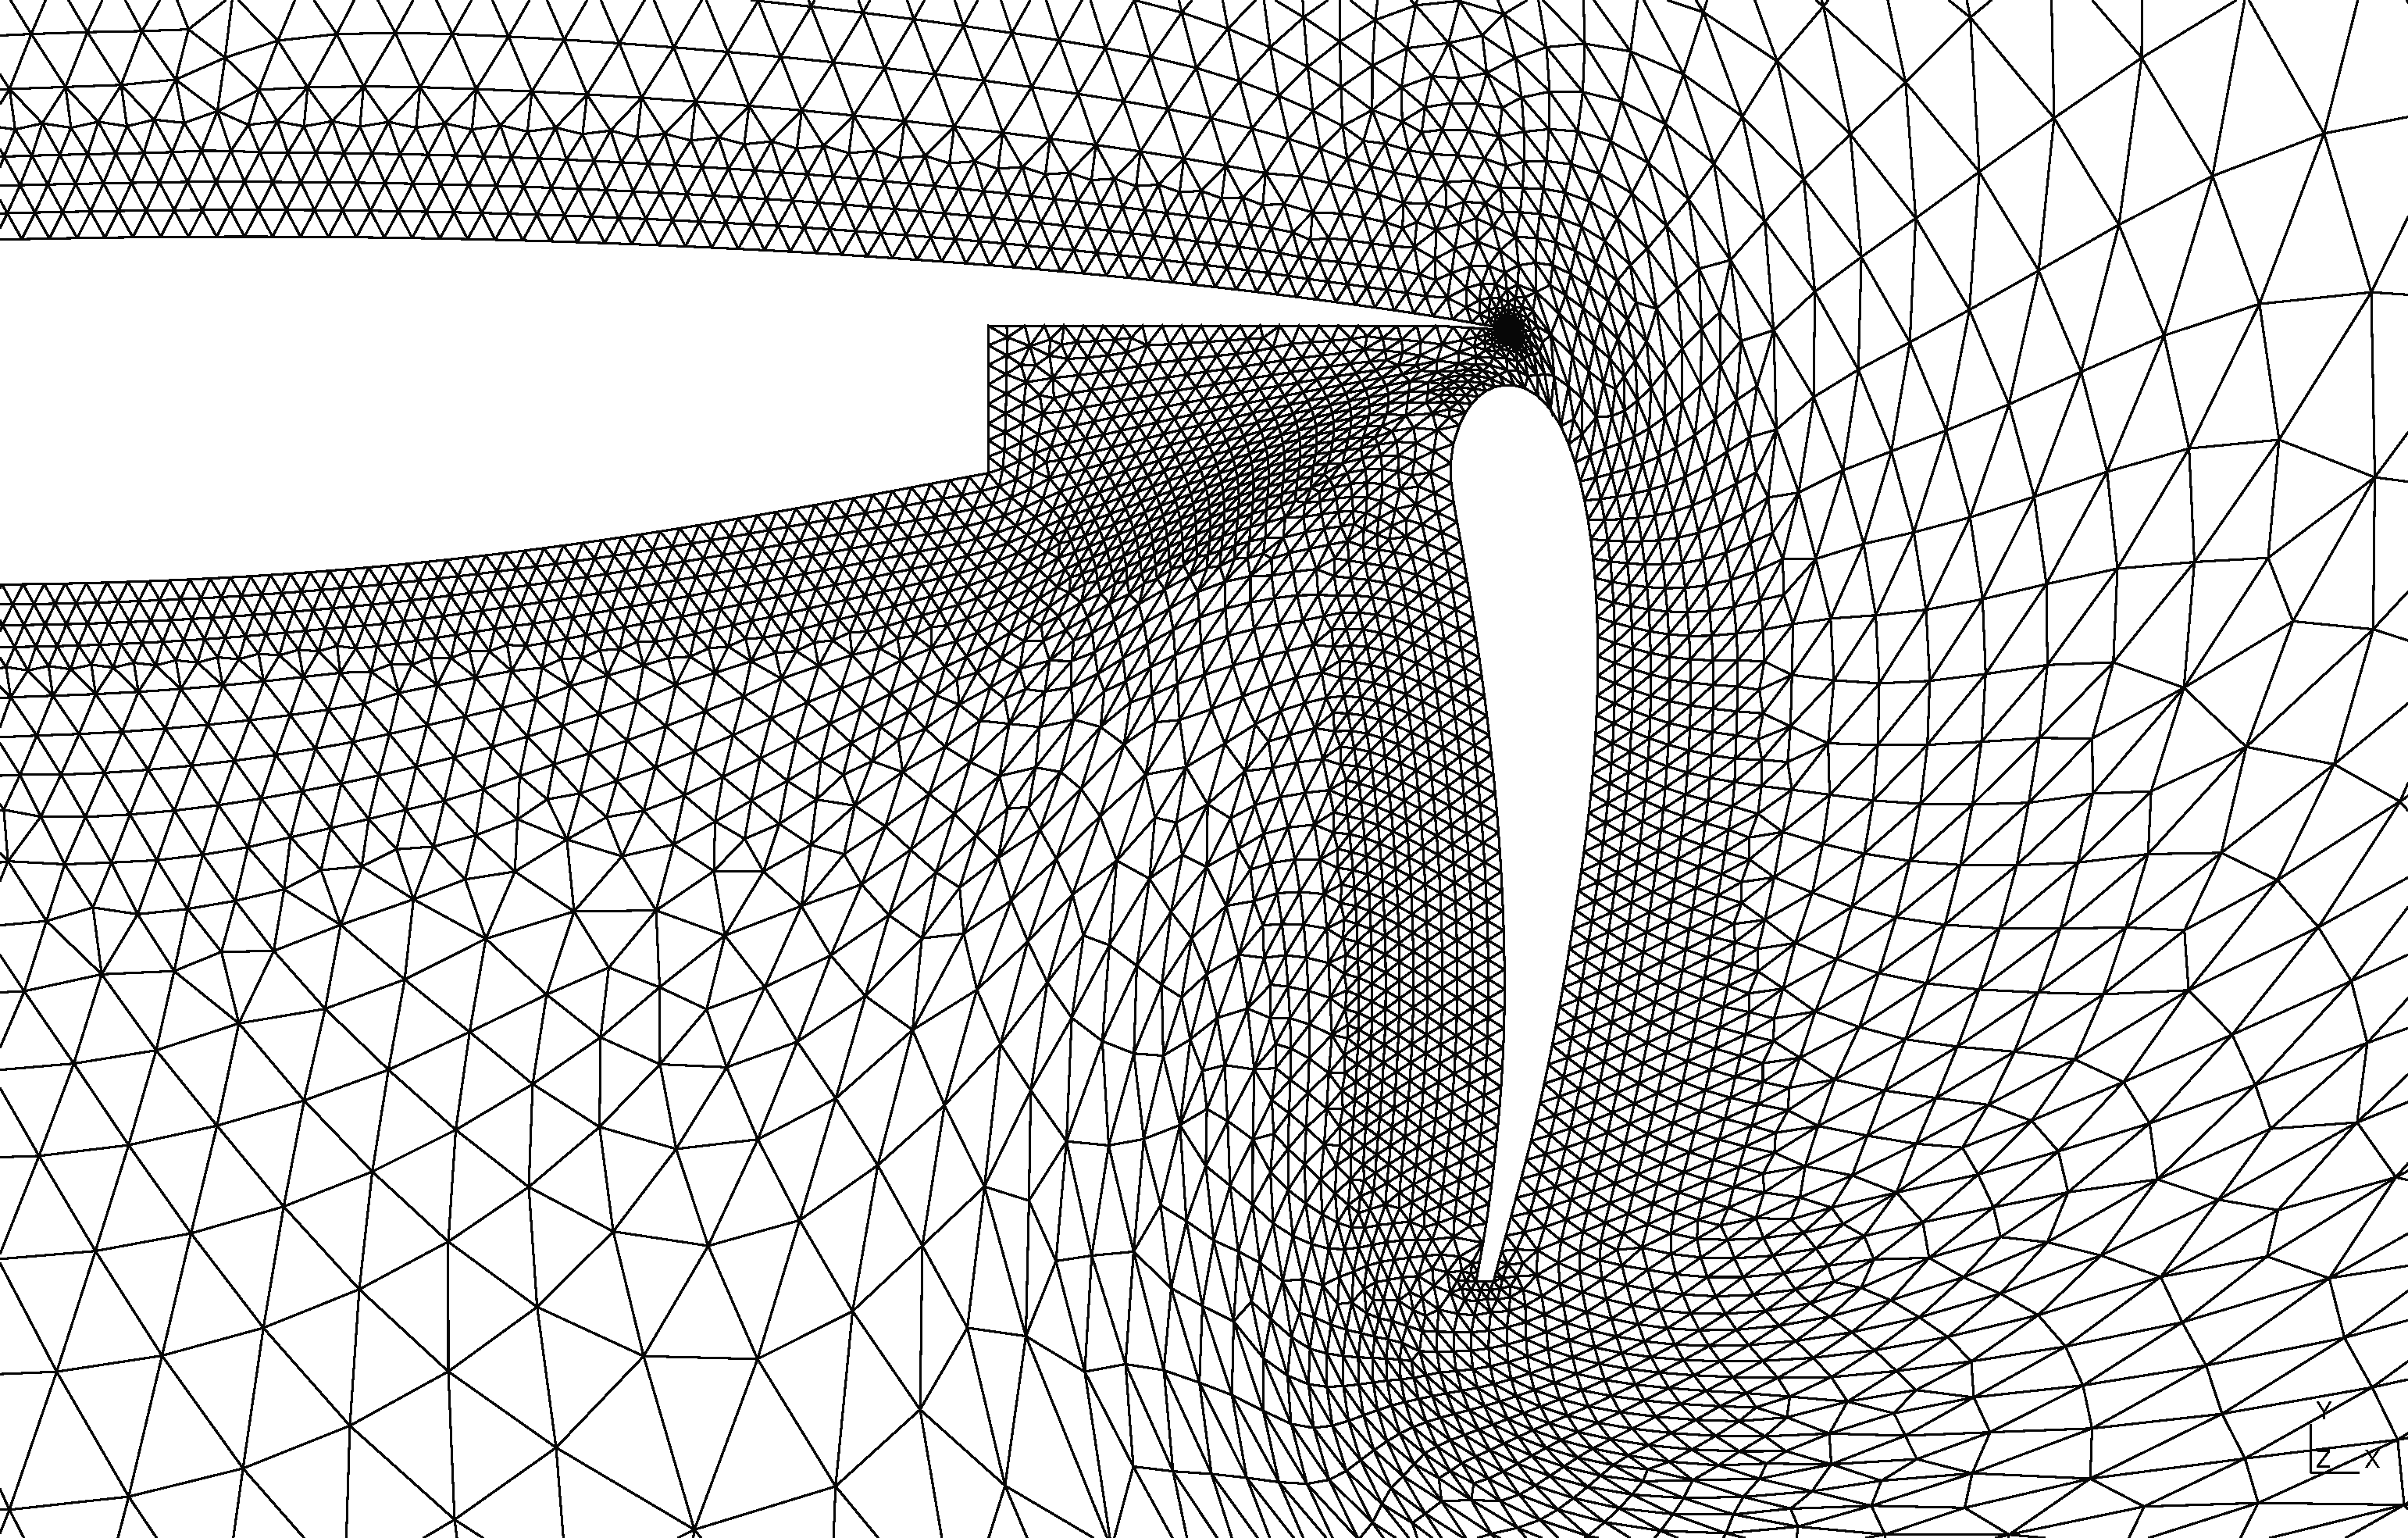
\includegraphics[scale=0.25]{wing60-rbf-sr15-s3}
	\caption{Inviscid 3-component airfoil mesh with 60$^\circ$ rotation of flap by RBF method}
	\label{fig:wing-inviscid-rbf}
\end{figure}
\begin{figure}
	\centering
	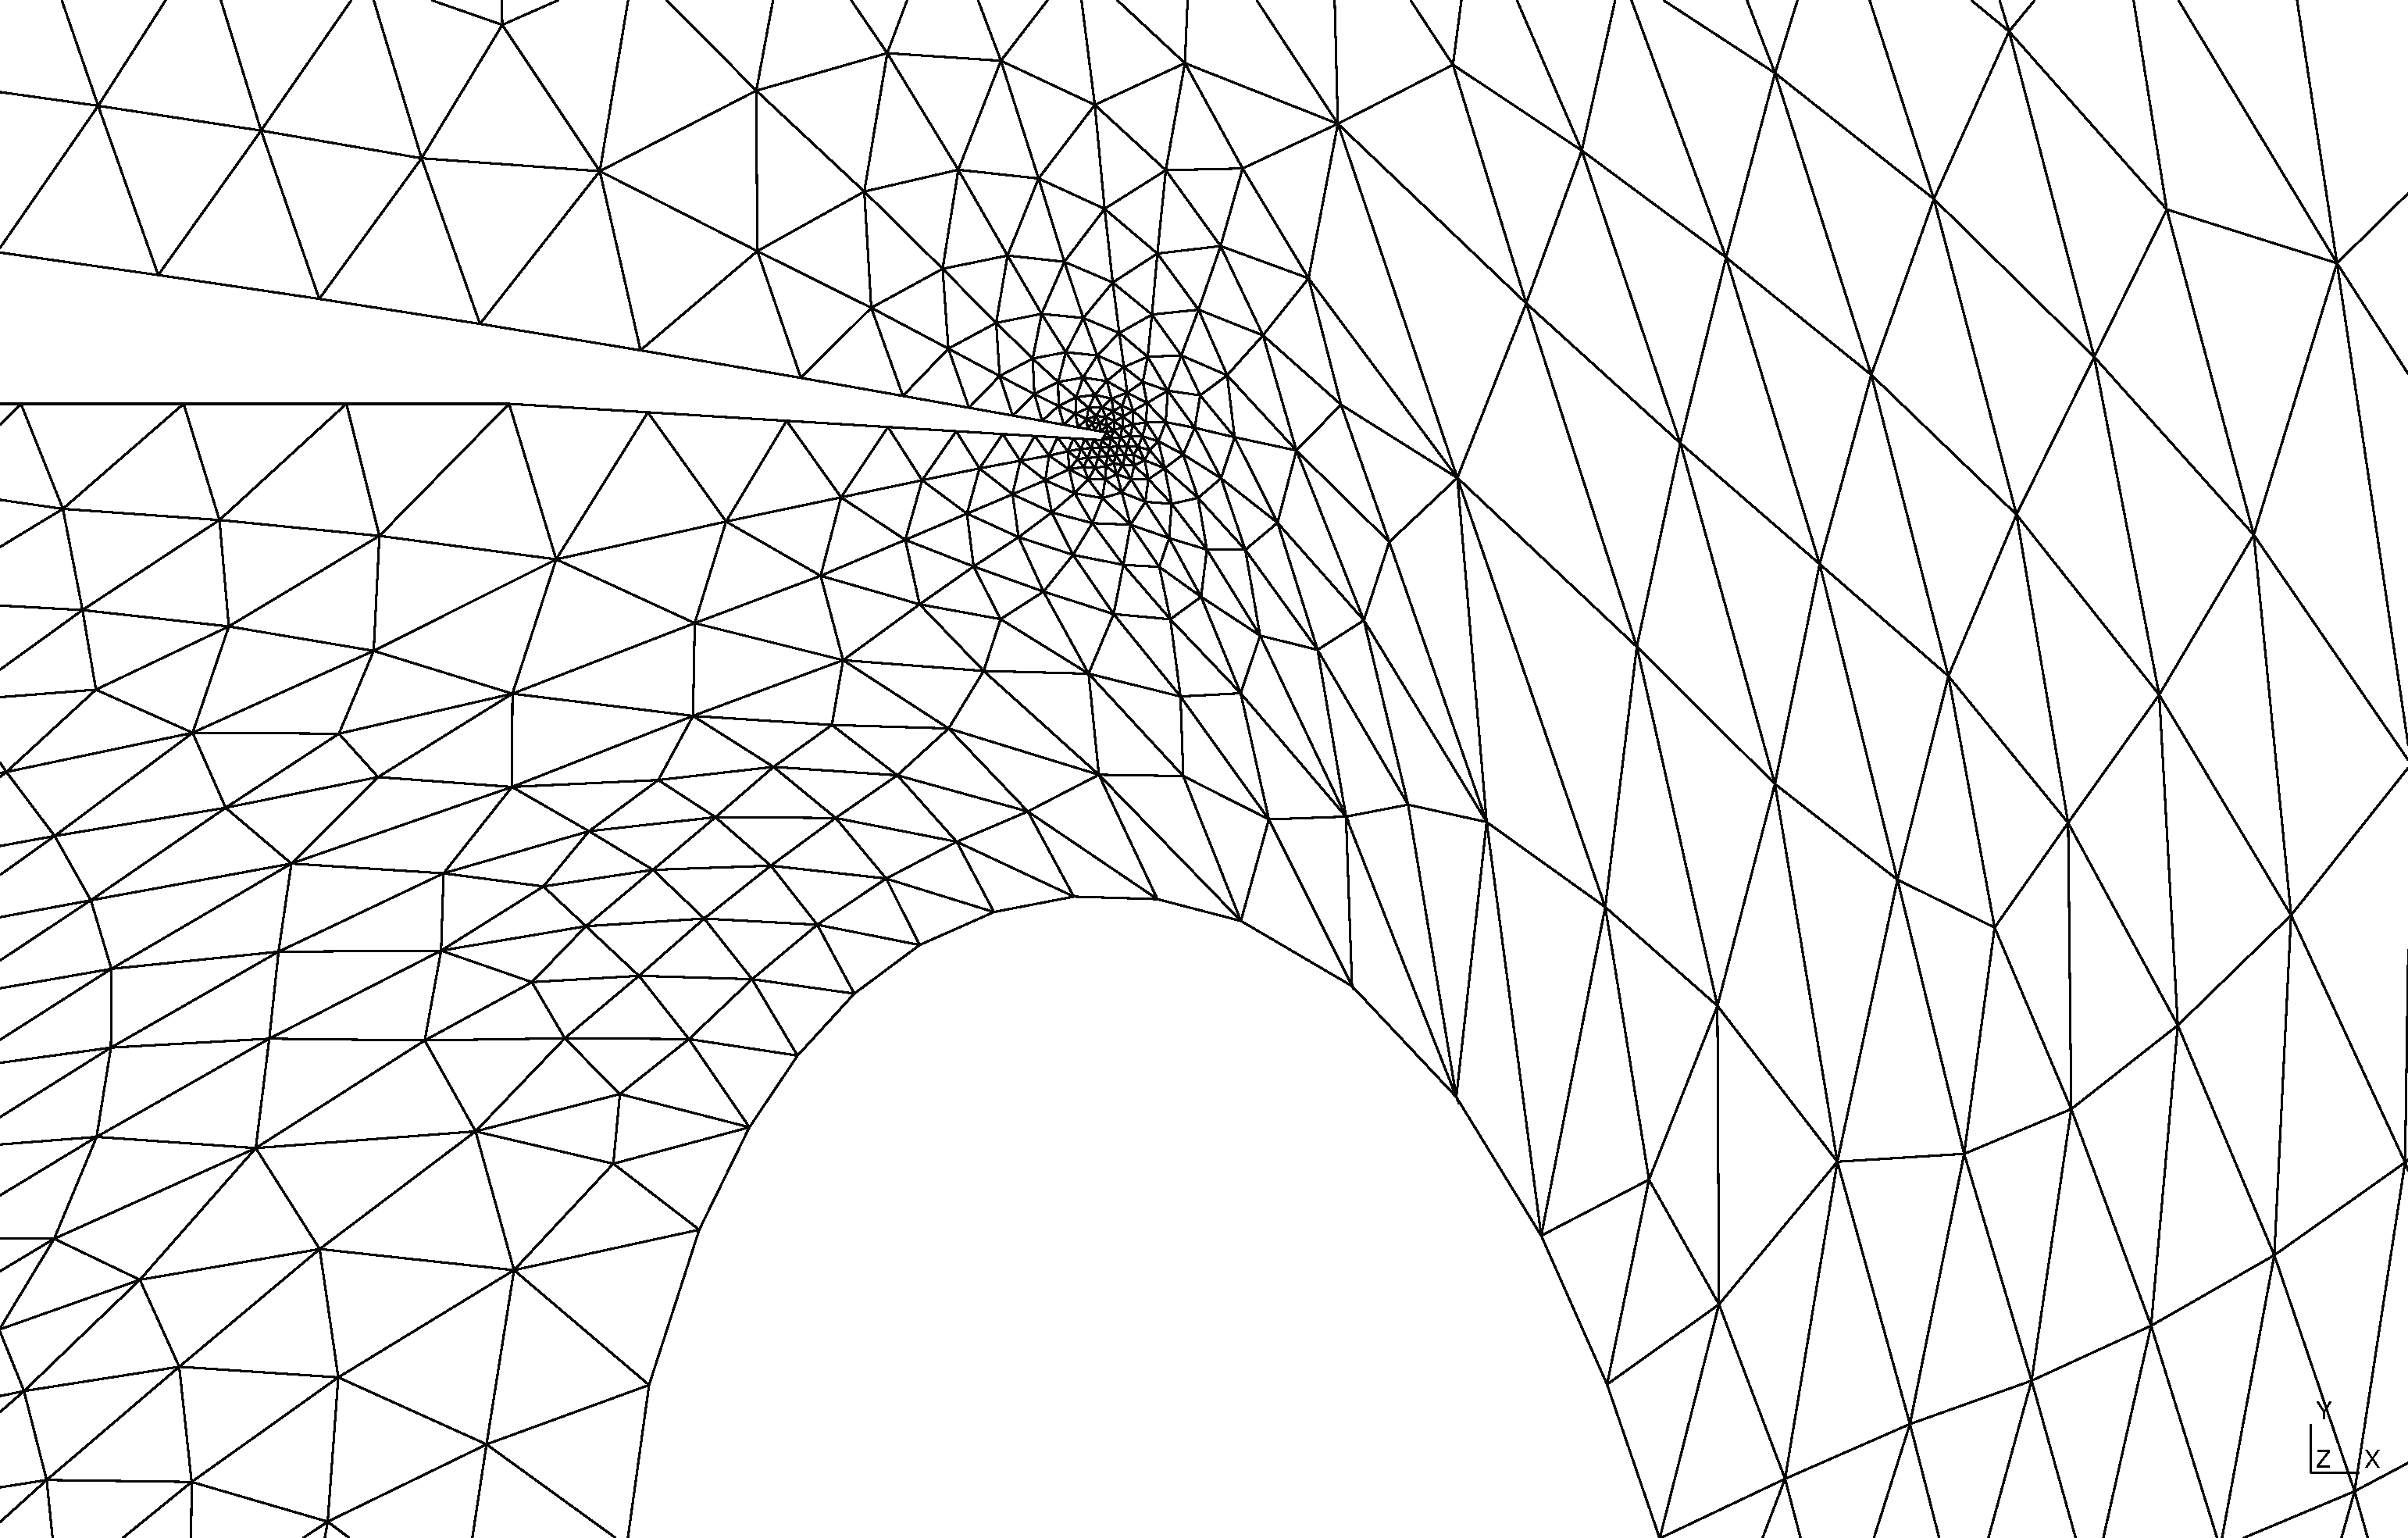
\includegraphics[scale=0.25]{wing60-rbf-sr15-s3_zoomed}
	\caption{Inviscid 3-component airfoil mesh with 60$^\circ$ rotation of flap by RBF method; zoomed to where the flap meets the wing}
	\label{fig:wing-inviscid-rbf-zoomed}
\end{figure}
\begin{figure}
	\centering
	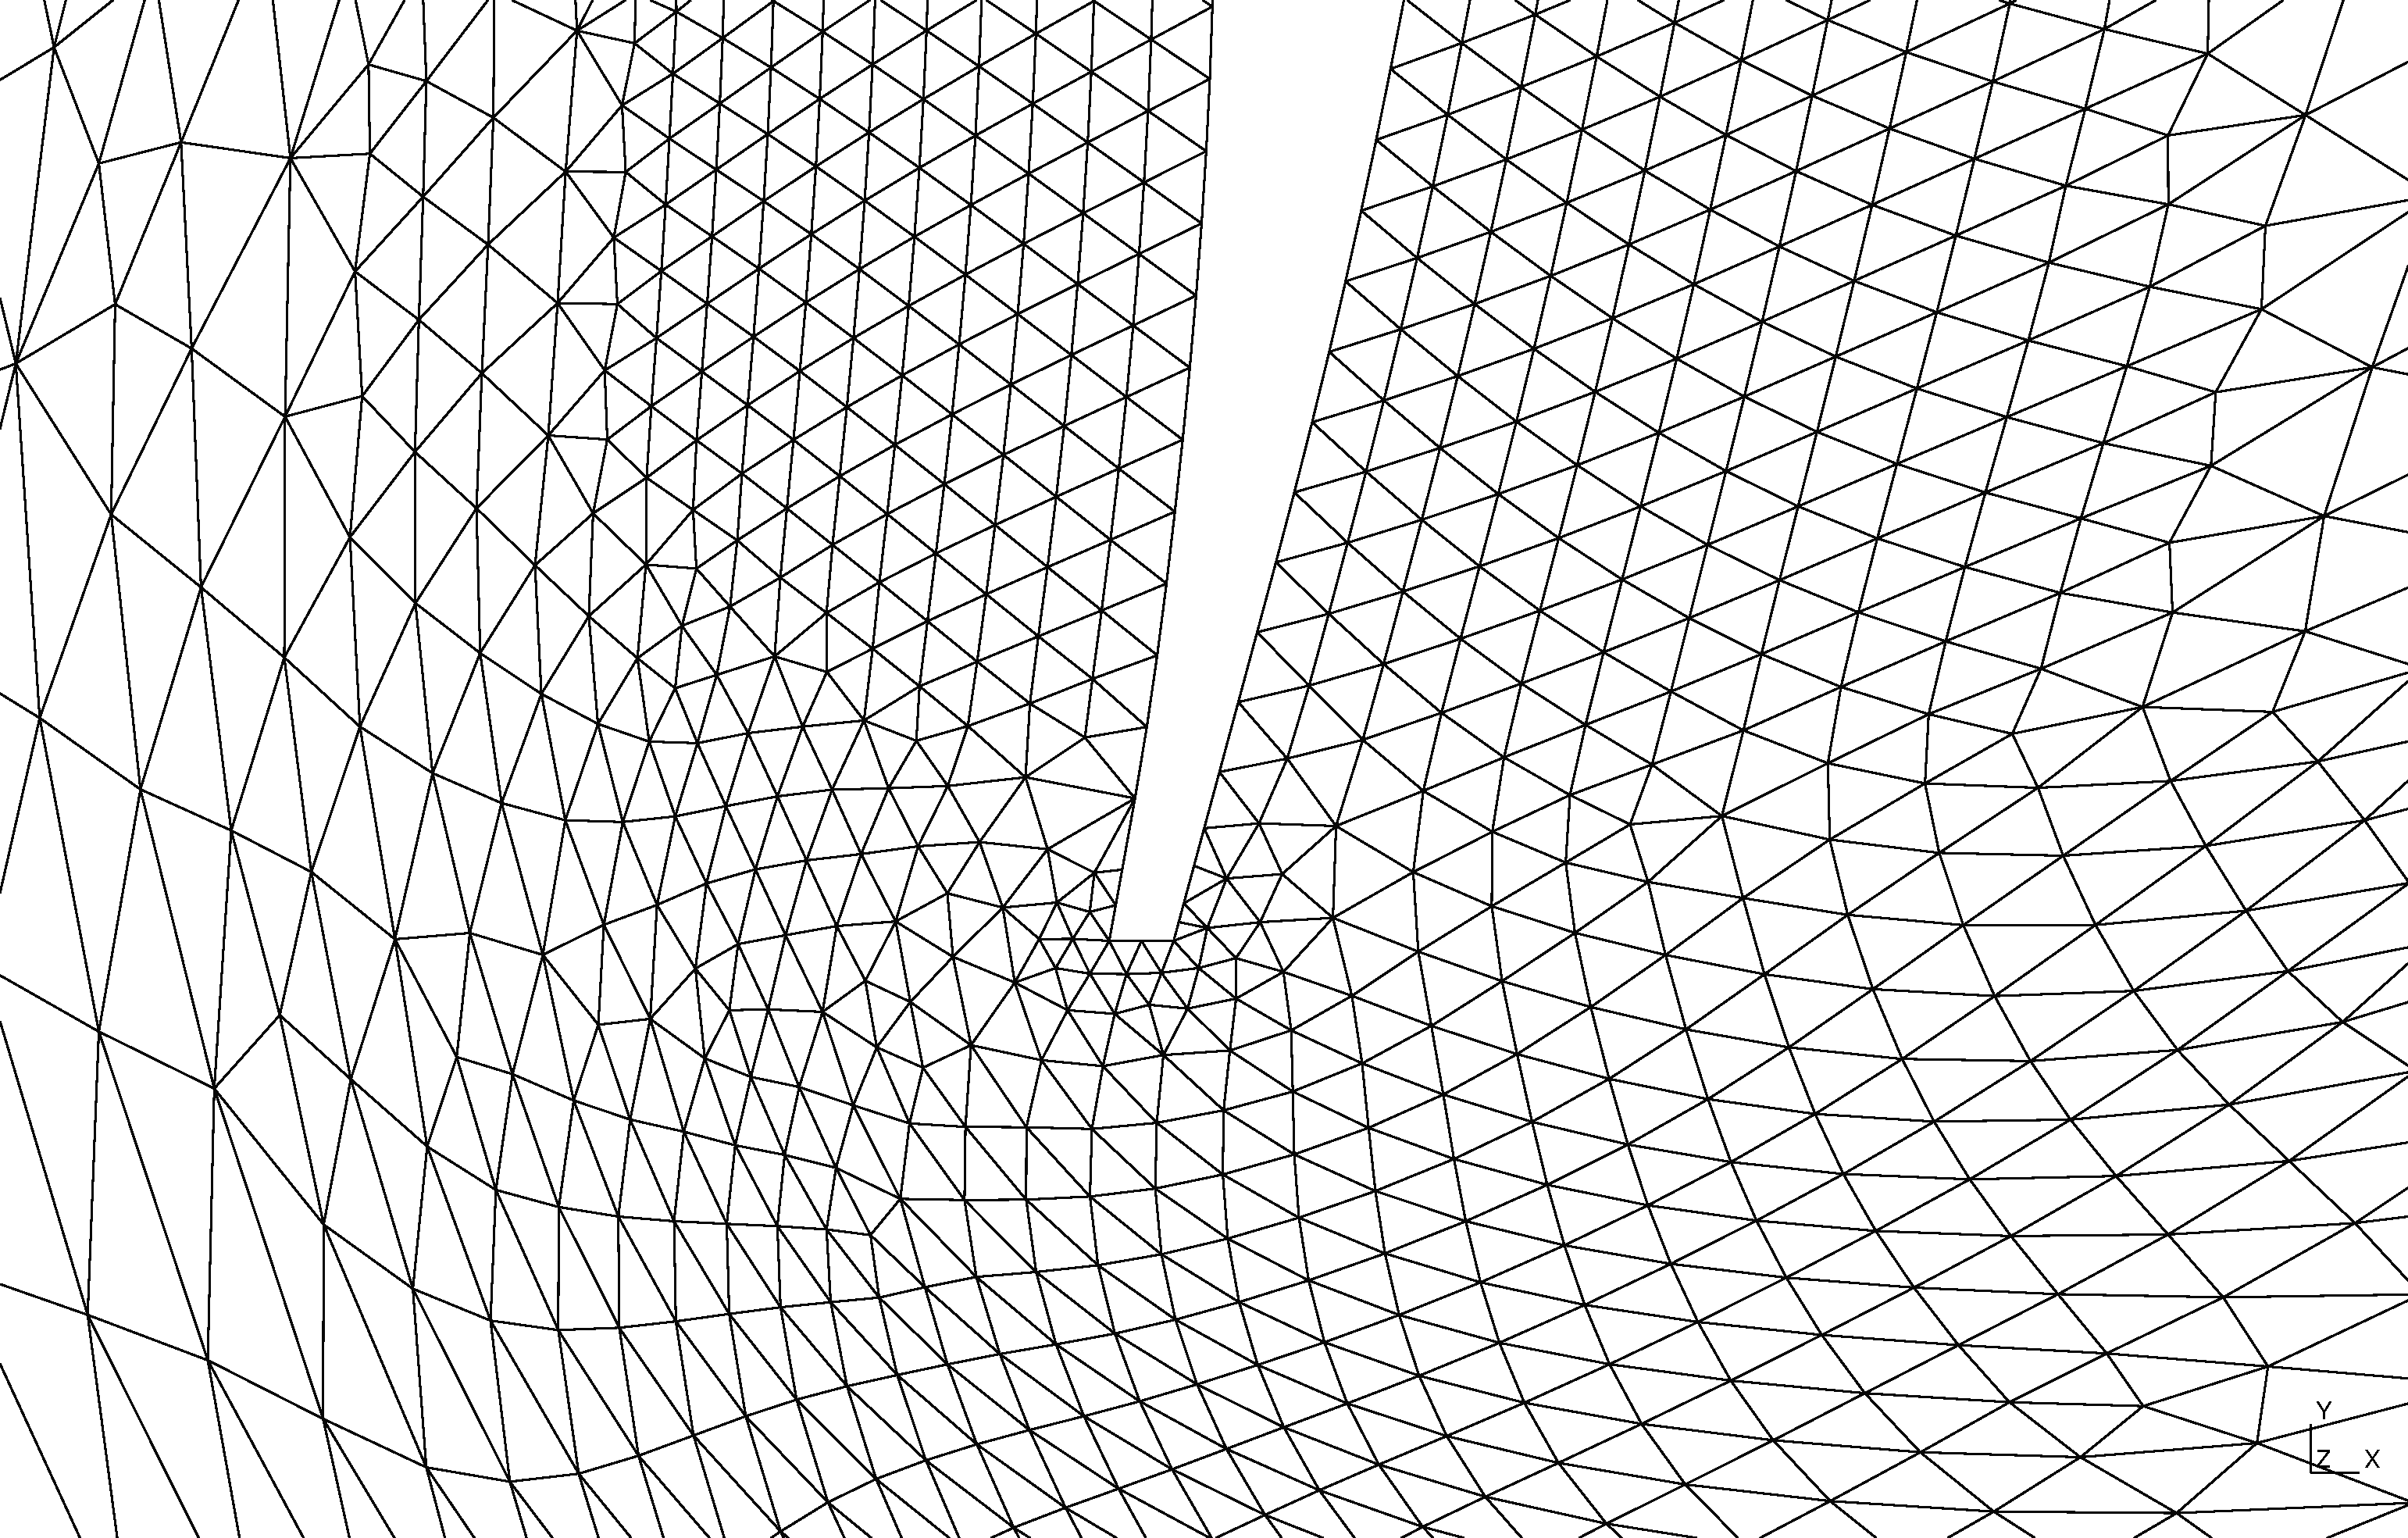
\includegraphics[scale=0.25]{wing60-rbf-sr15-s3_zoomed2}
	\caption{Inviscid 3-component airfoil mesh with 60$^\circ$ rotation of flap by RBF method, zoomed to the trailing edge of the flap}
	\label{fig:wing-inviscid-rbf-zoomed2}
\end{figure}
 
\FloatBarrier

 We present a case of rotation of an interior object inside a far-field boundary using interpolation methods on a quadrilateral mesh. The skew metric has been computed for this case. We show results for a 60-degree rotation in case of DGM (fig. \ref{fig:qin-60-dgm}), RBF (fig. \ref{fig:qin-60-rbf}) and DG-RBF2 (fig. \ref{fig:qin-60-dgrbf2}) methods. Note that DGRBF2 refers to the interpolation of rotation angles by DGRBF. The case has been referred from Wang \emph{et. al.} \cite{mm:dgrbf}. Figure \ref{fig:qin-orig} shows the un-deformed mesh.
 
 \begin{figure}
 	\centering
 	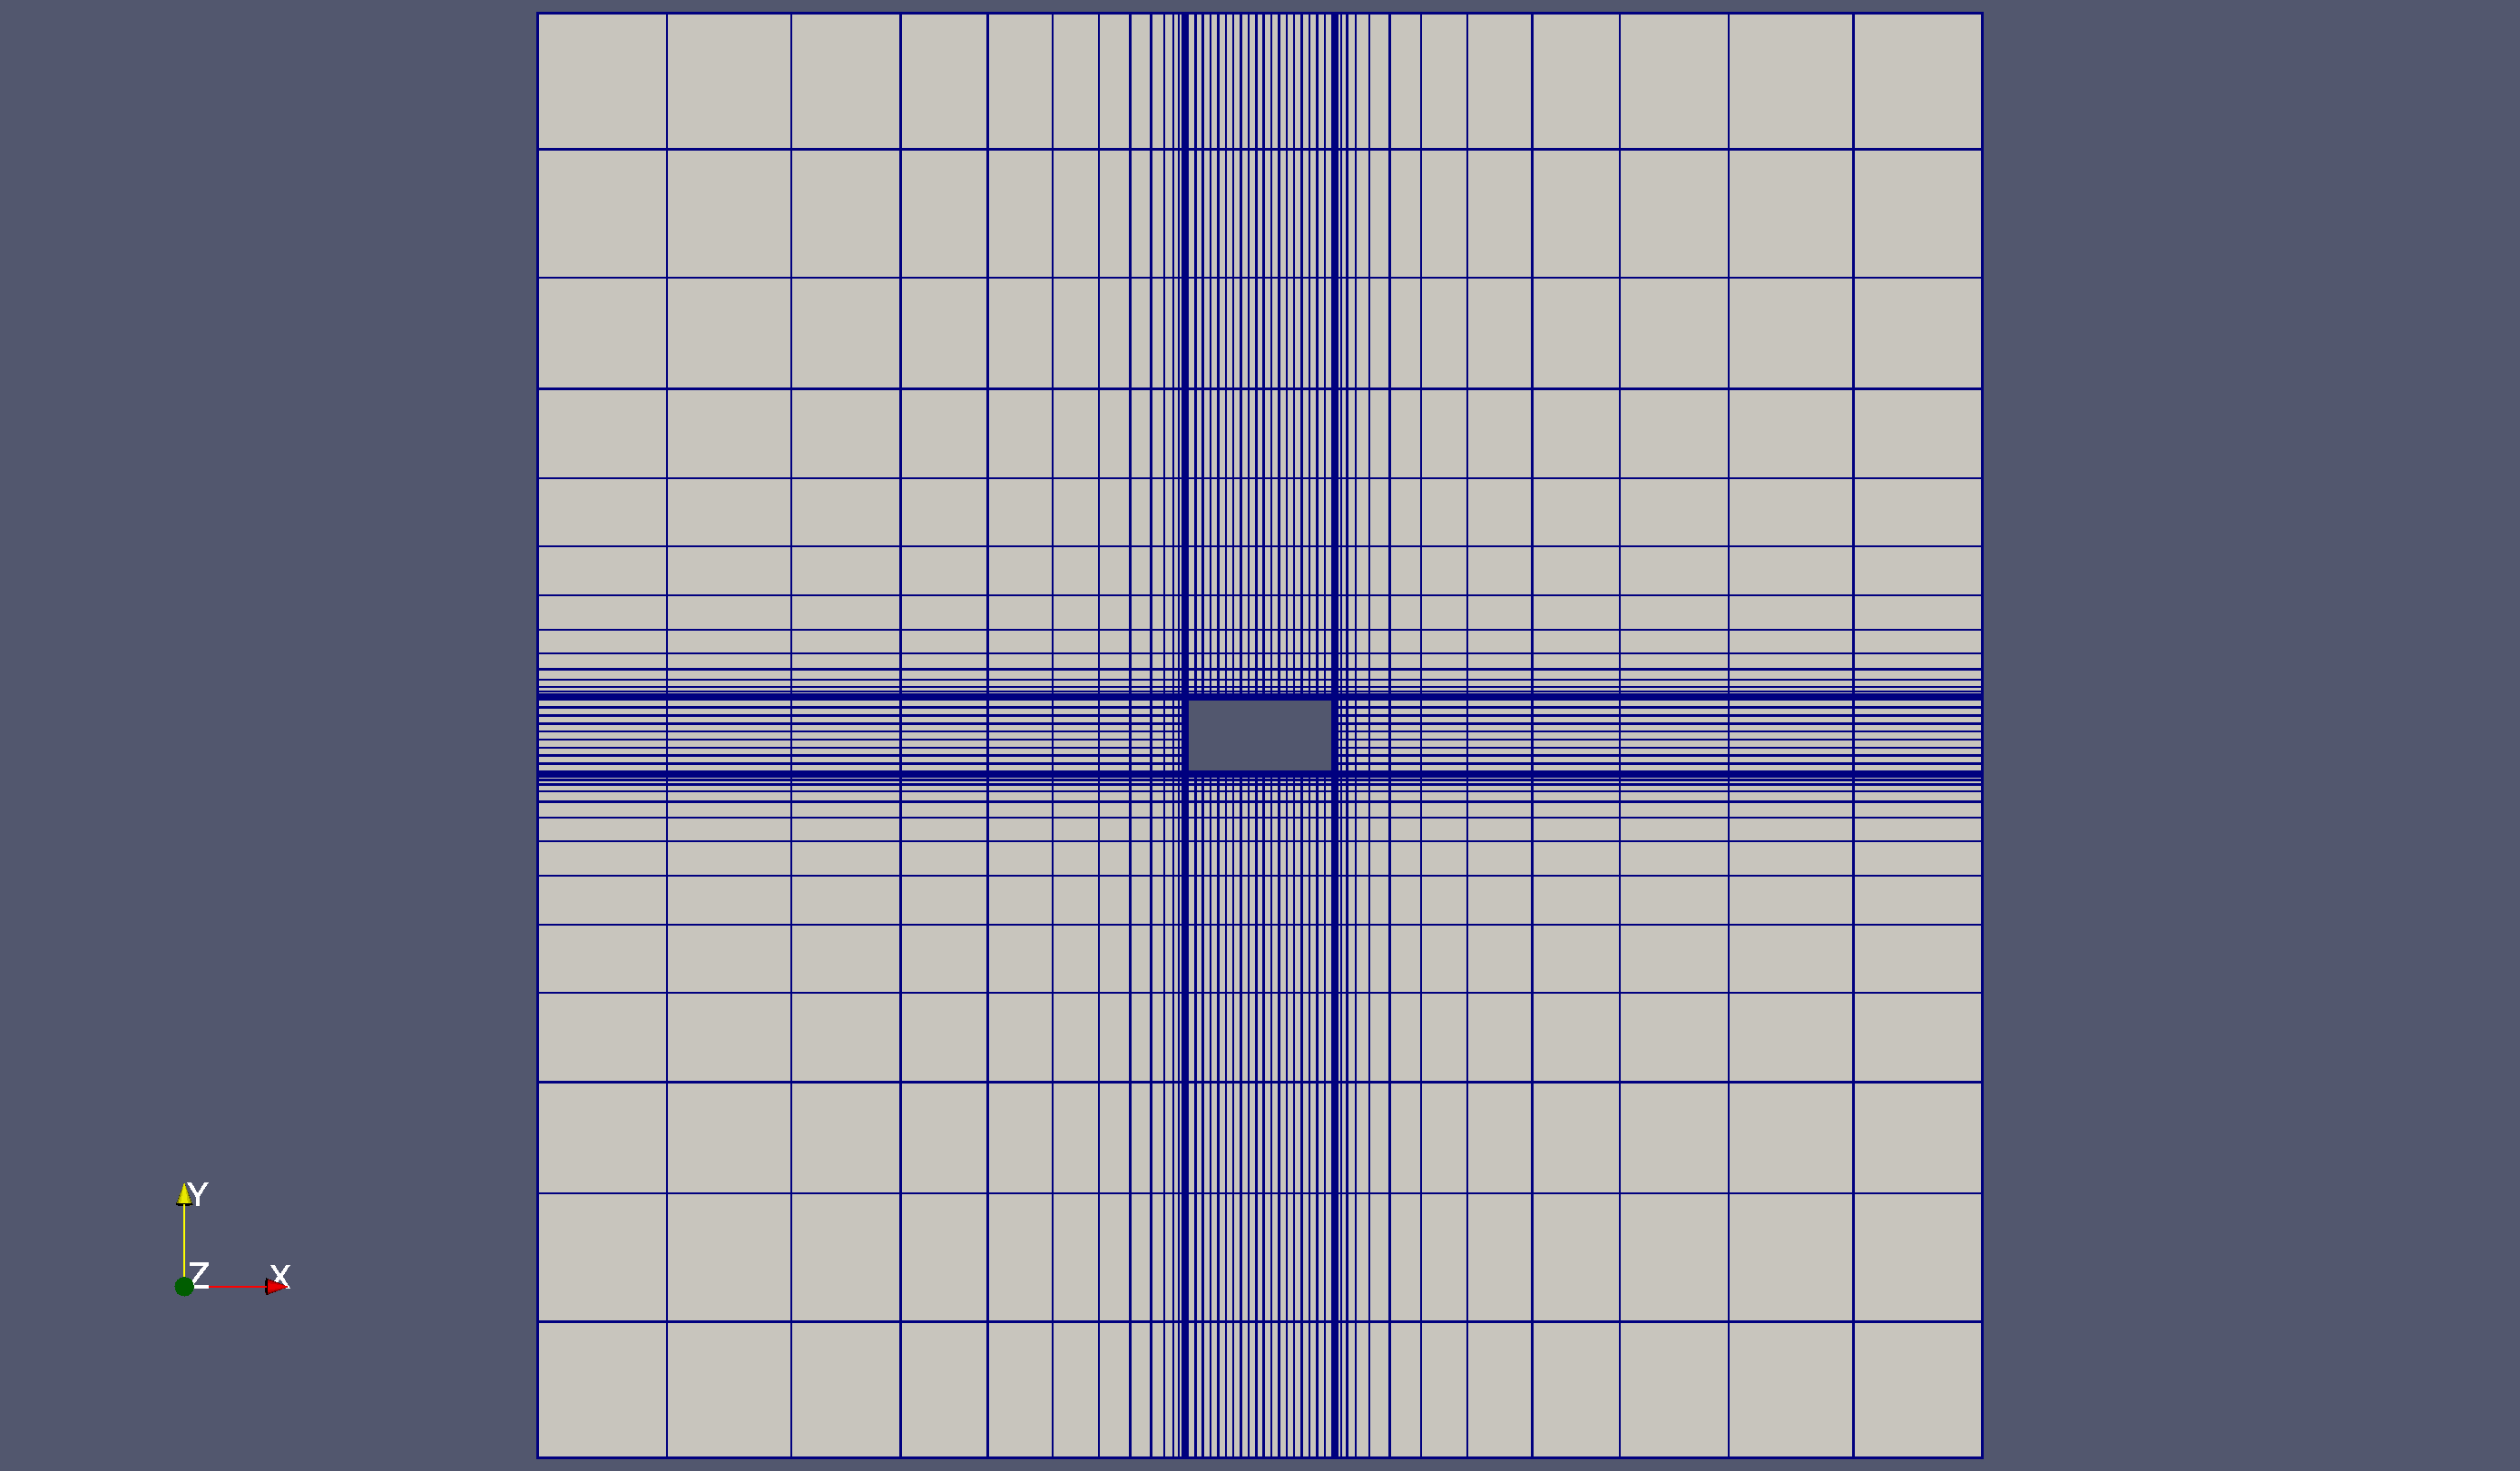
\includegraphics[scale=0.25]{qin-orig-mesh.pdf}
 	\caption{Original mesh}
 	\label{fig:qin-orig}
 \end{figure}
 
 \begin{figure}
 	\centering
 	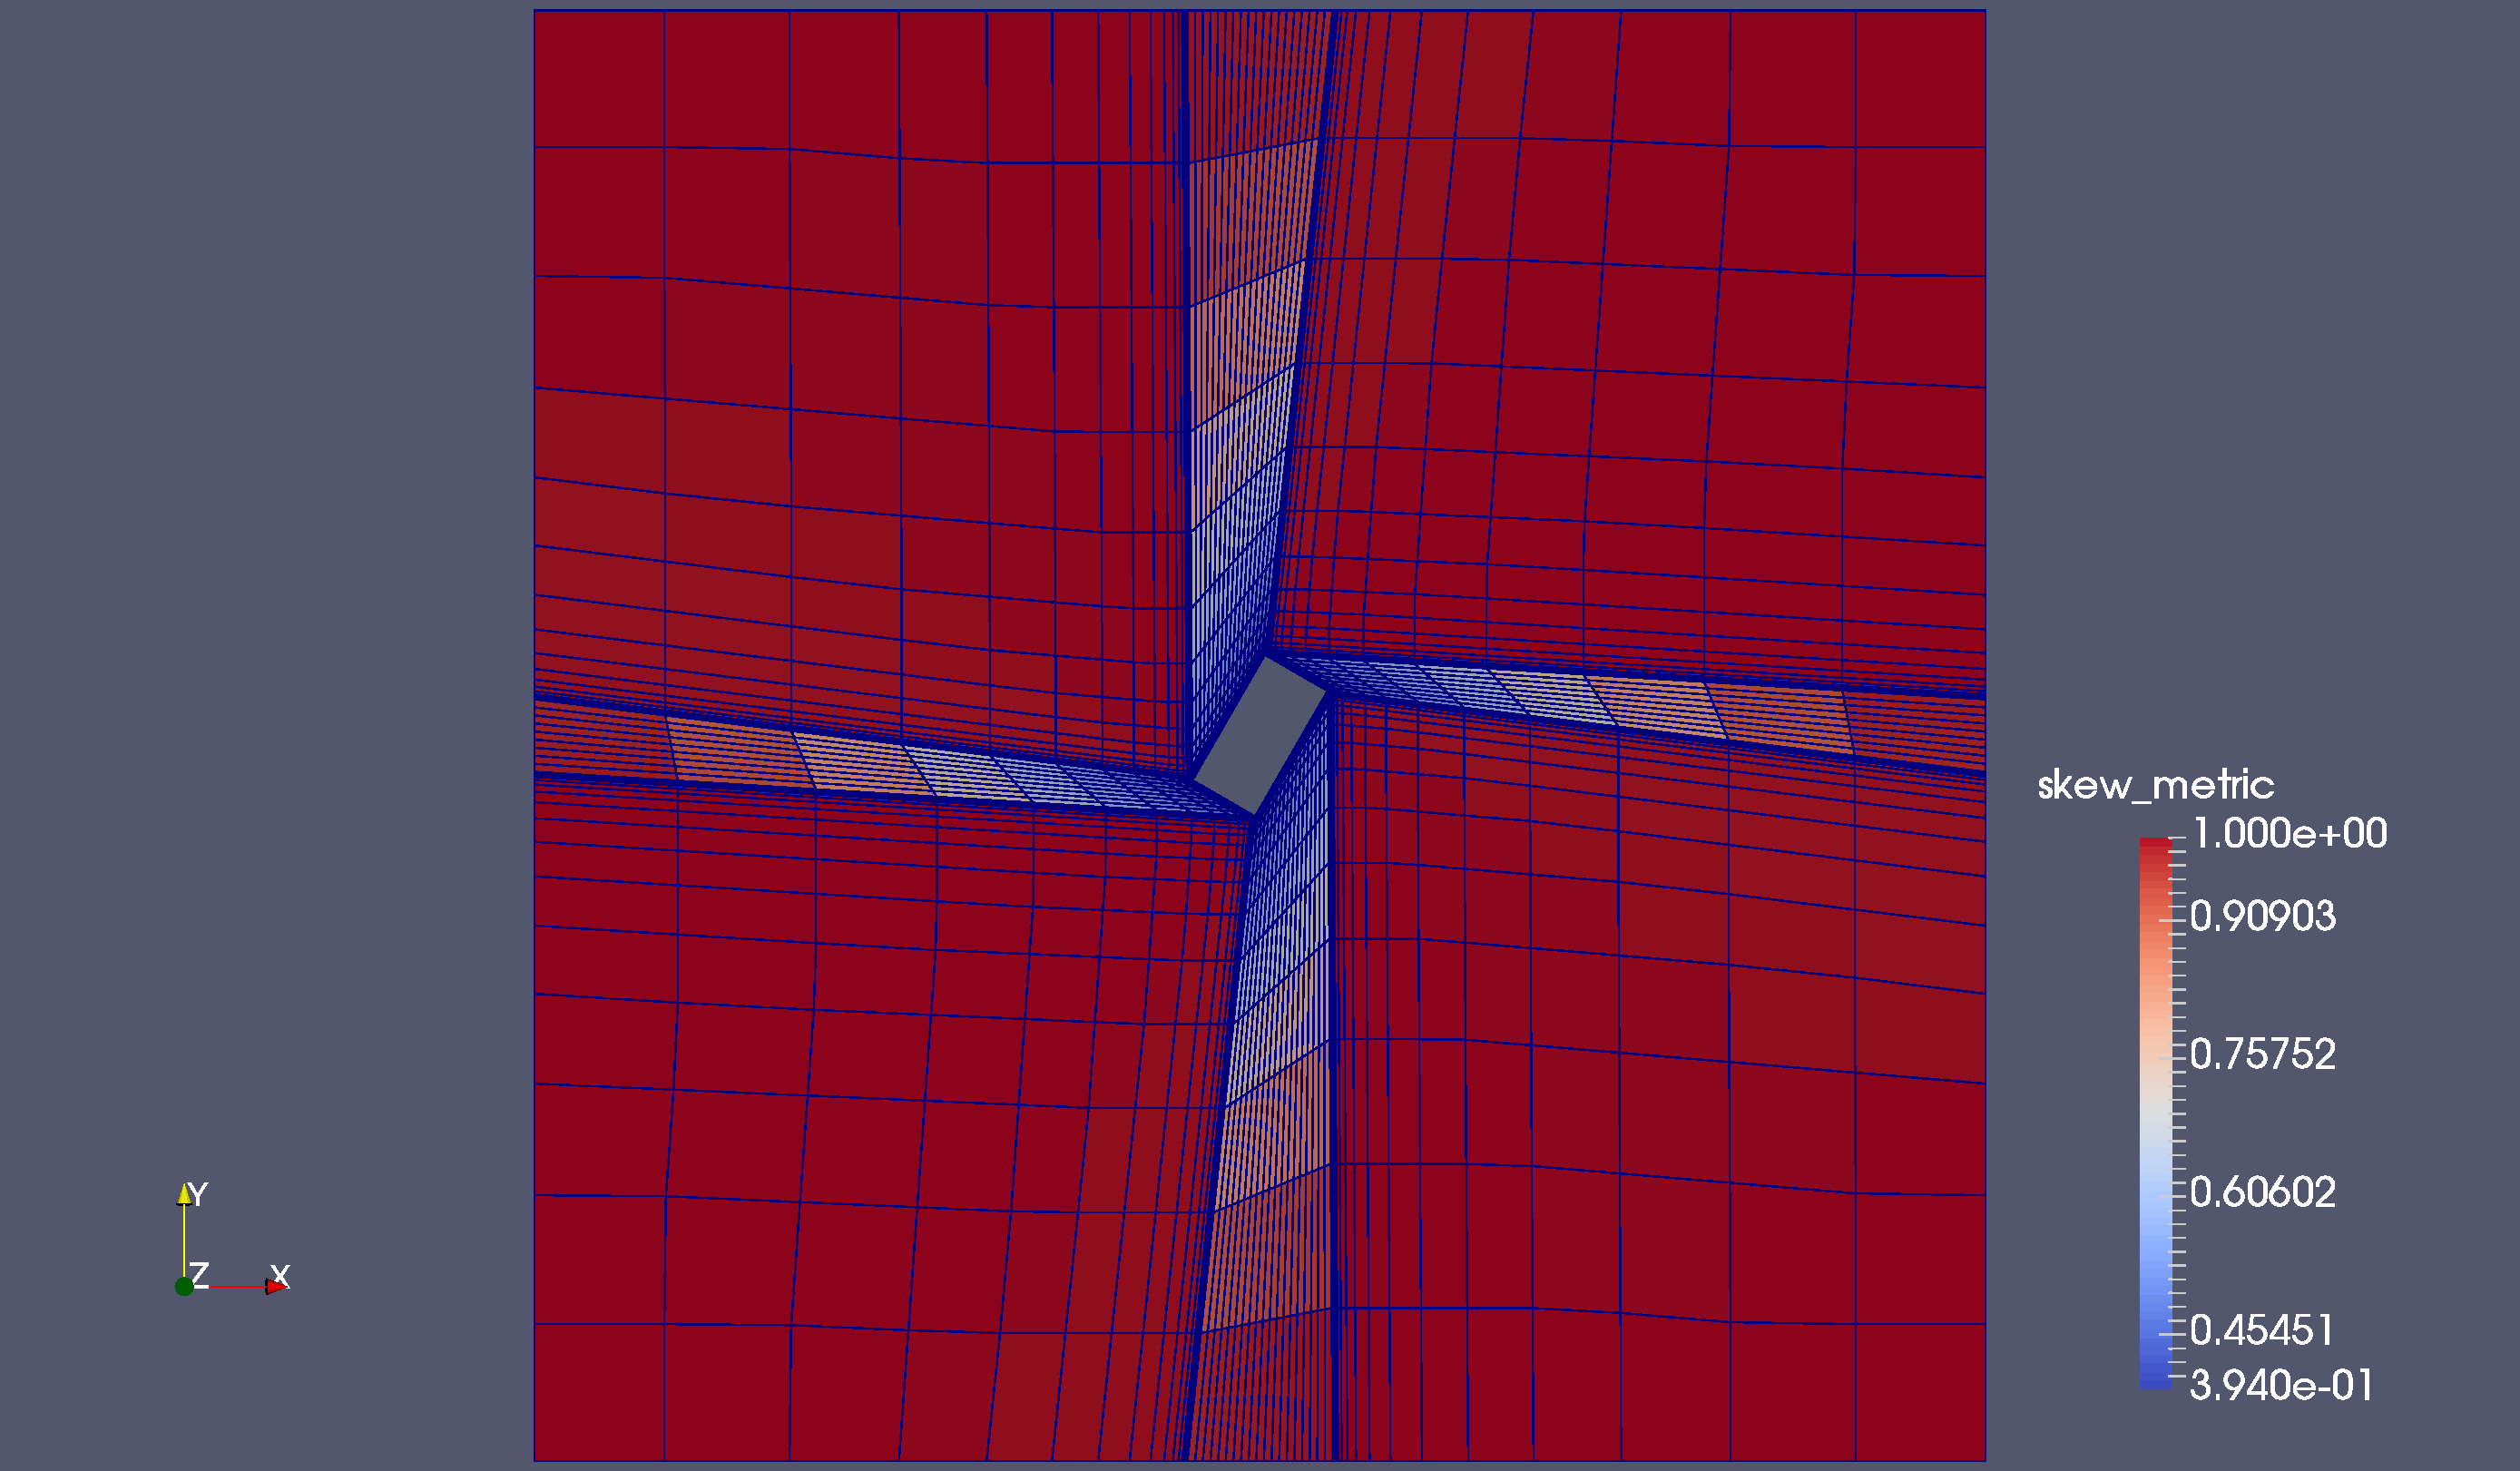
\includegraphics[scale=0.25]{qin-60-dgm-quality.pdf}
 	\caption{60 degrees rotation by DGM}
 	\label{fig:qin-60-dgm}
 \end{figure}
 
 \begin{figure}
 	\centering
 	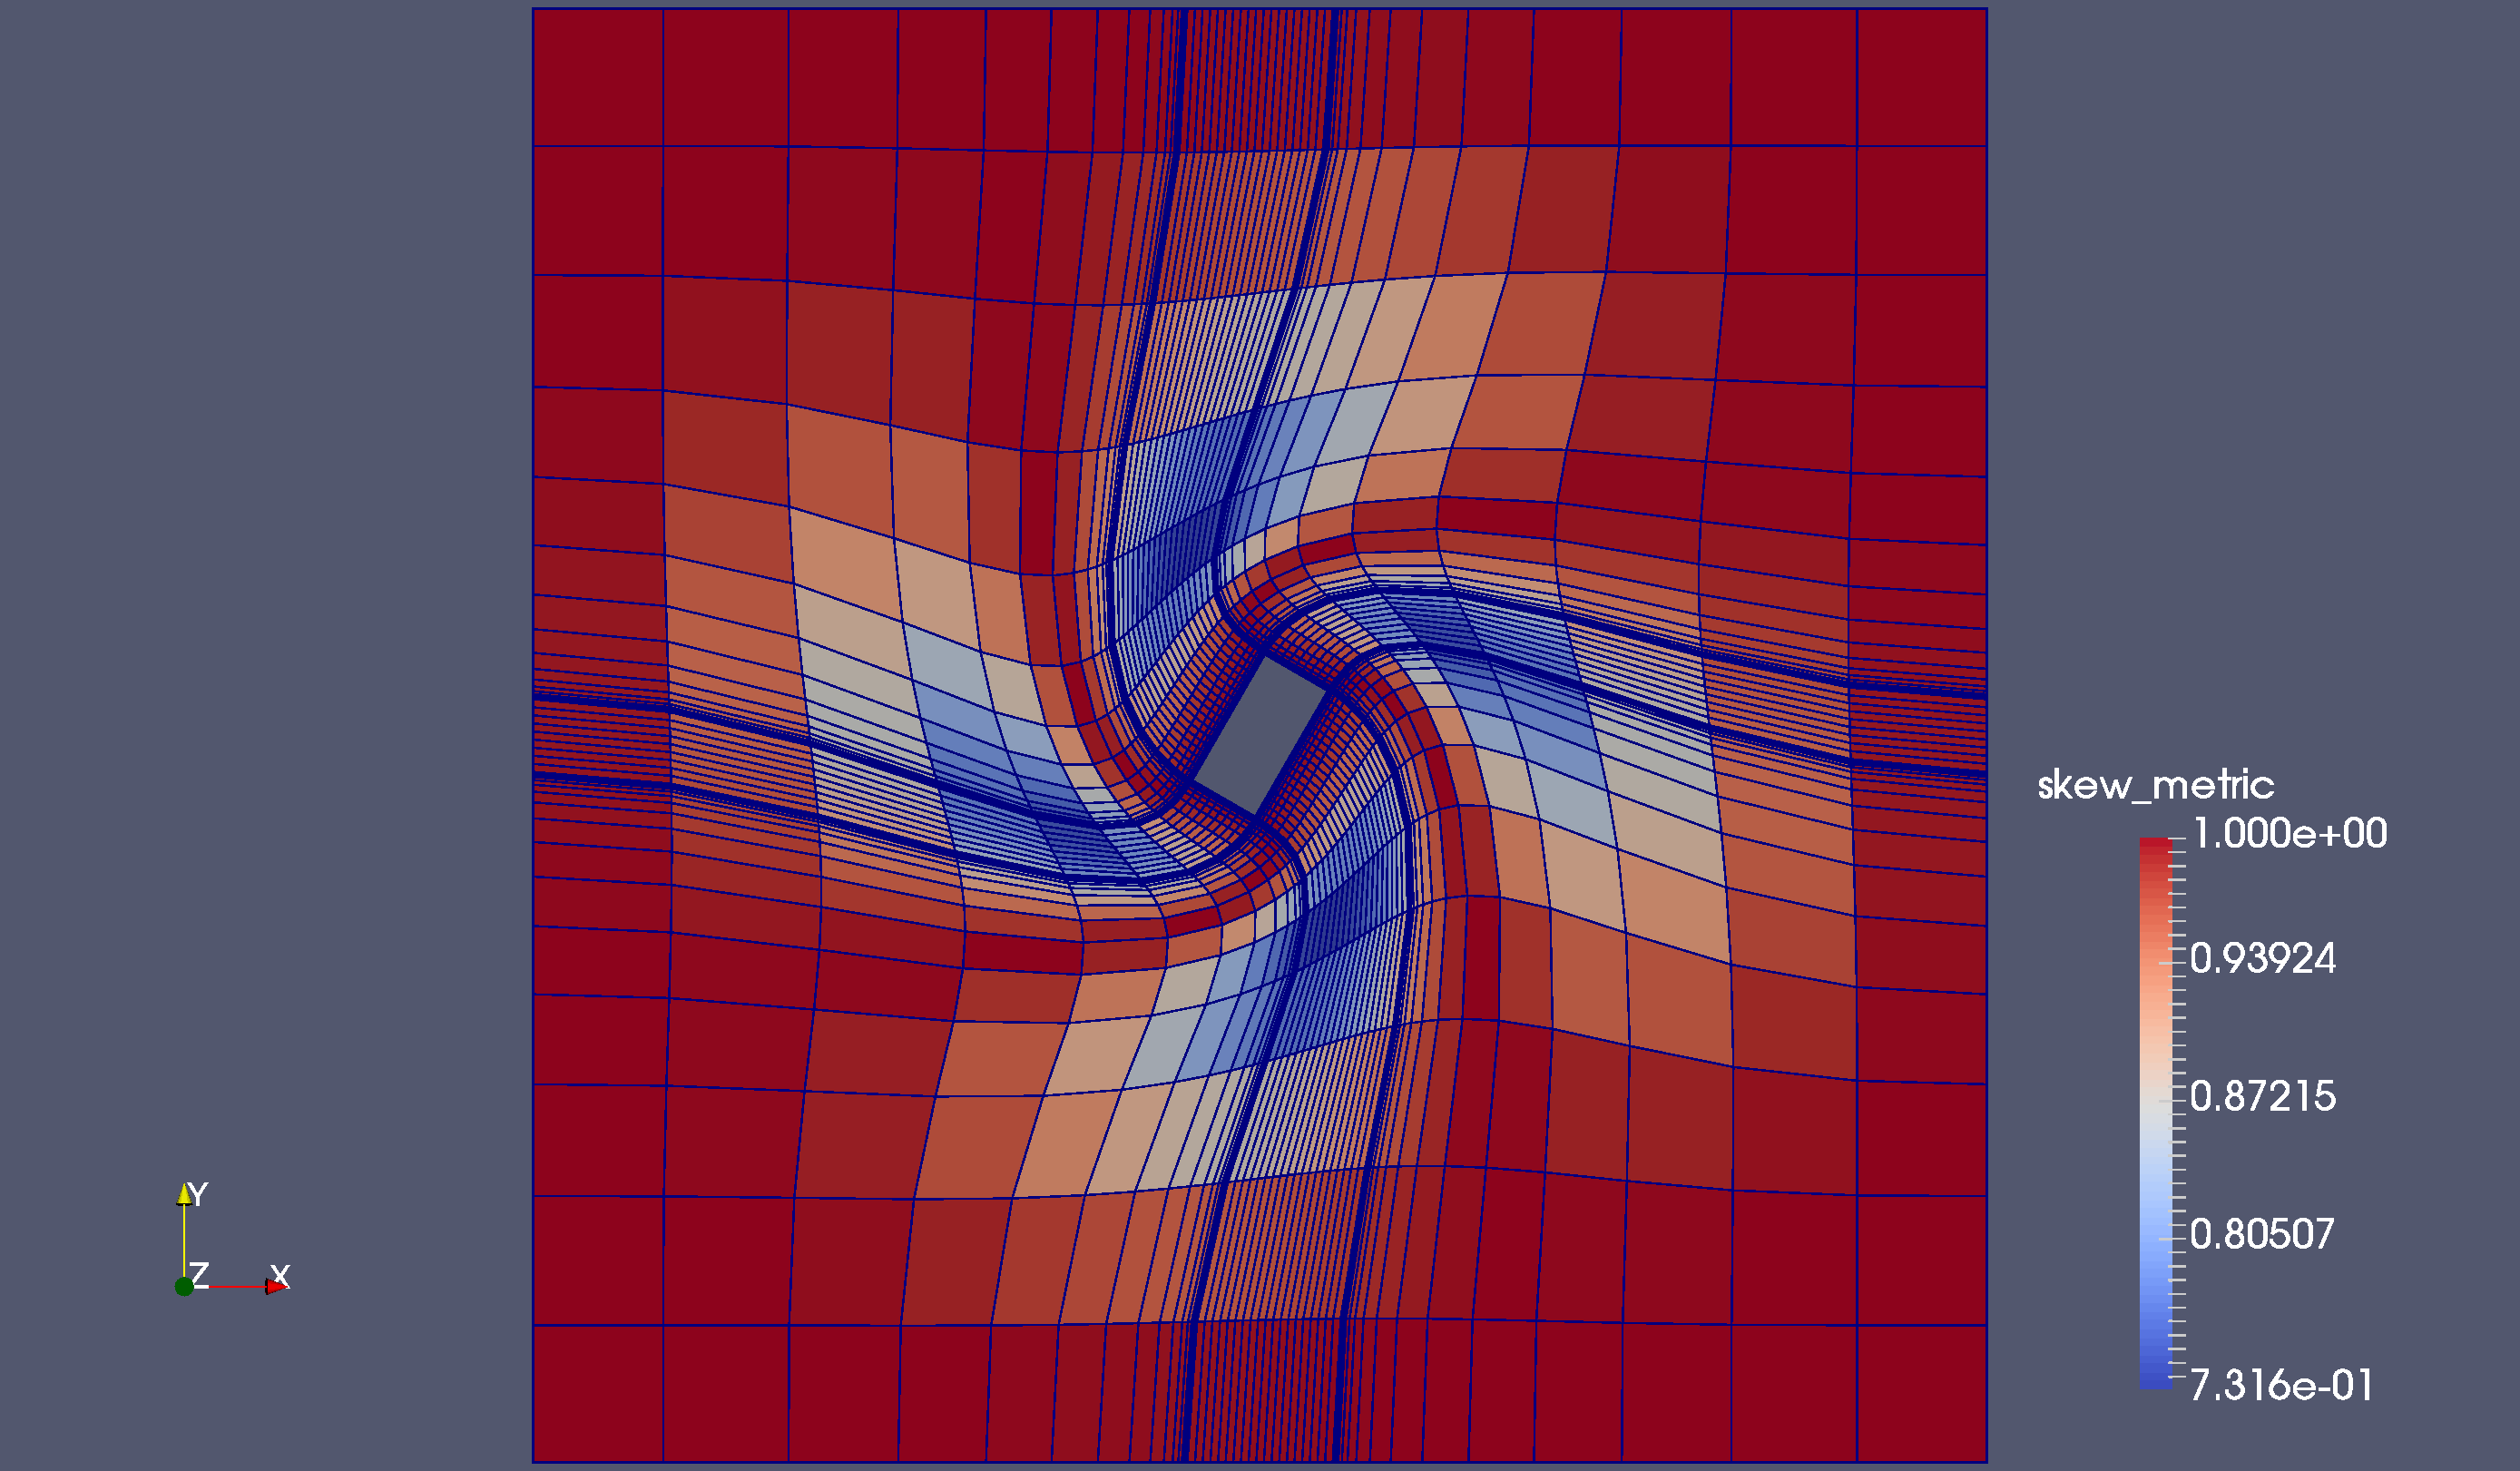
\includegraphics[scale=0.25]{qin-60-rbf-quality.pdf}
 	\caption{60 degrees rotation by RBF}
 	\label{fig:qin-60-rbf}
 \end{figure}
 
 \begin{figure}
 	\centering
 	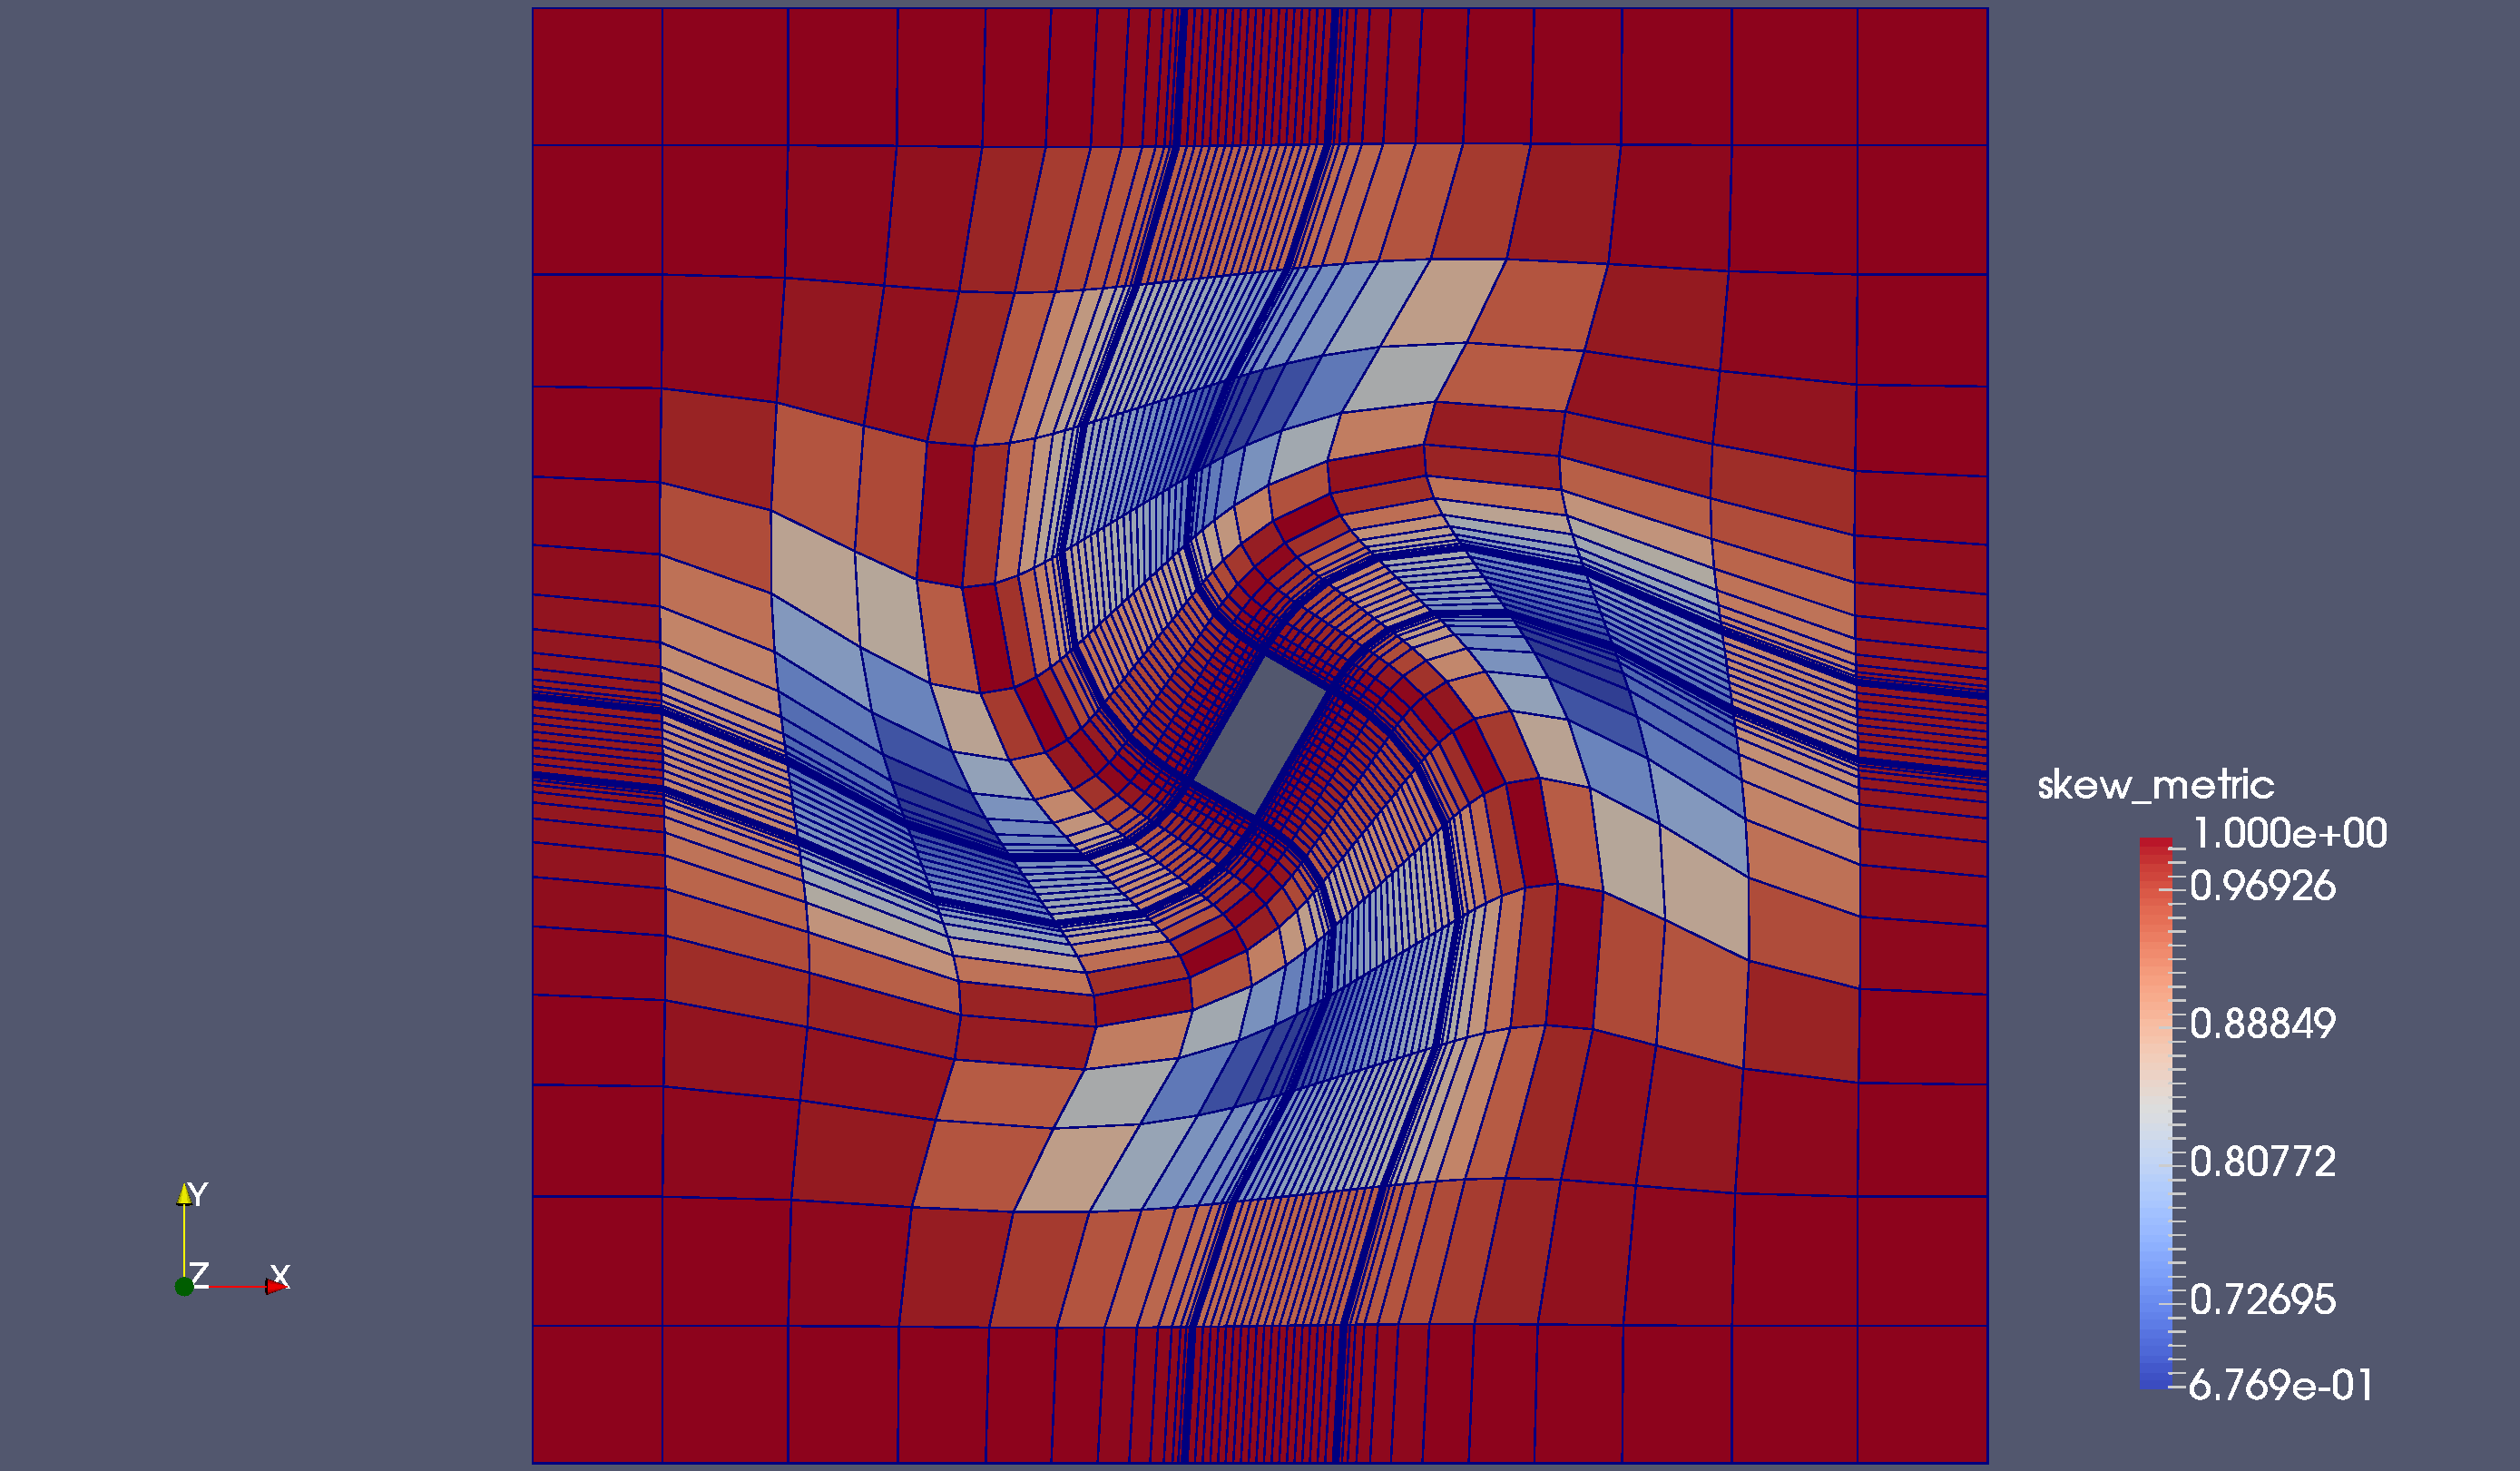
\includegraphics[scale=0.25]{qin-60-dgrbf2-quality.pdf}
 	\caption{60 degrees rotation by DGRBF2}
 	\label{fig:qin-60-dgrbf2}
 \end{figure}
 
 We note that the RBF and DGRBF2 methods can handle the rotation case quite well. The high-aspect-ratio elements near the inner boundaries are well-preserved, while the elements further in the interior, which are larger and can thus take more deformation, are distorted somewhat. Though RBF gives slightly better mesh quality than DGRBF2 for this amount of rotation, RBF takes 1.926 seconds of total CPU time (using conjugate gradient solver), while DGRBF2 takes only 0.08 seconds of total CPU time. Further, shown in figure \ref{fig:qin-dgrbf2-120} is a case of extreme rotation of 120 degrees, which DGRBF2 solves while maintaining mesh validity. None of the other methods are able to do this. RBF has been found to give valid meshes upto about 110 degrees of rotation. However, since DGRBF2 requires specification of rotation angles at boundary nodes, the method can be difficult to apply to general complex motions.
 
 \begin{figure}
 	\centering
 	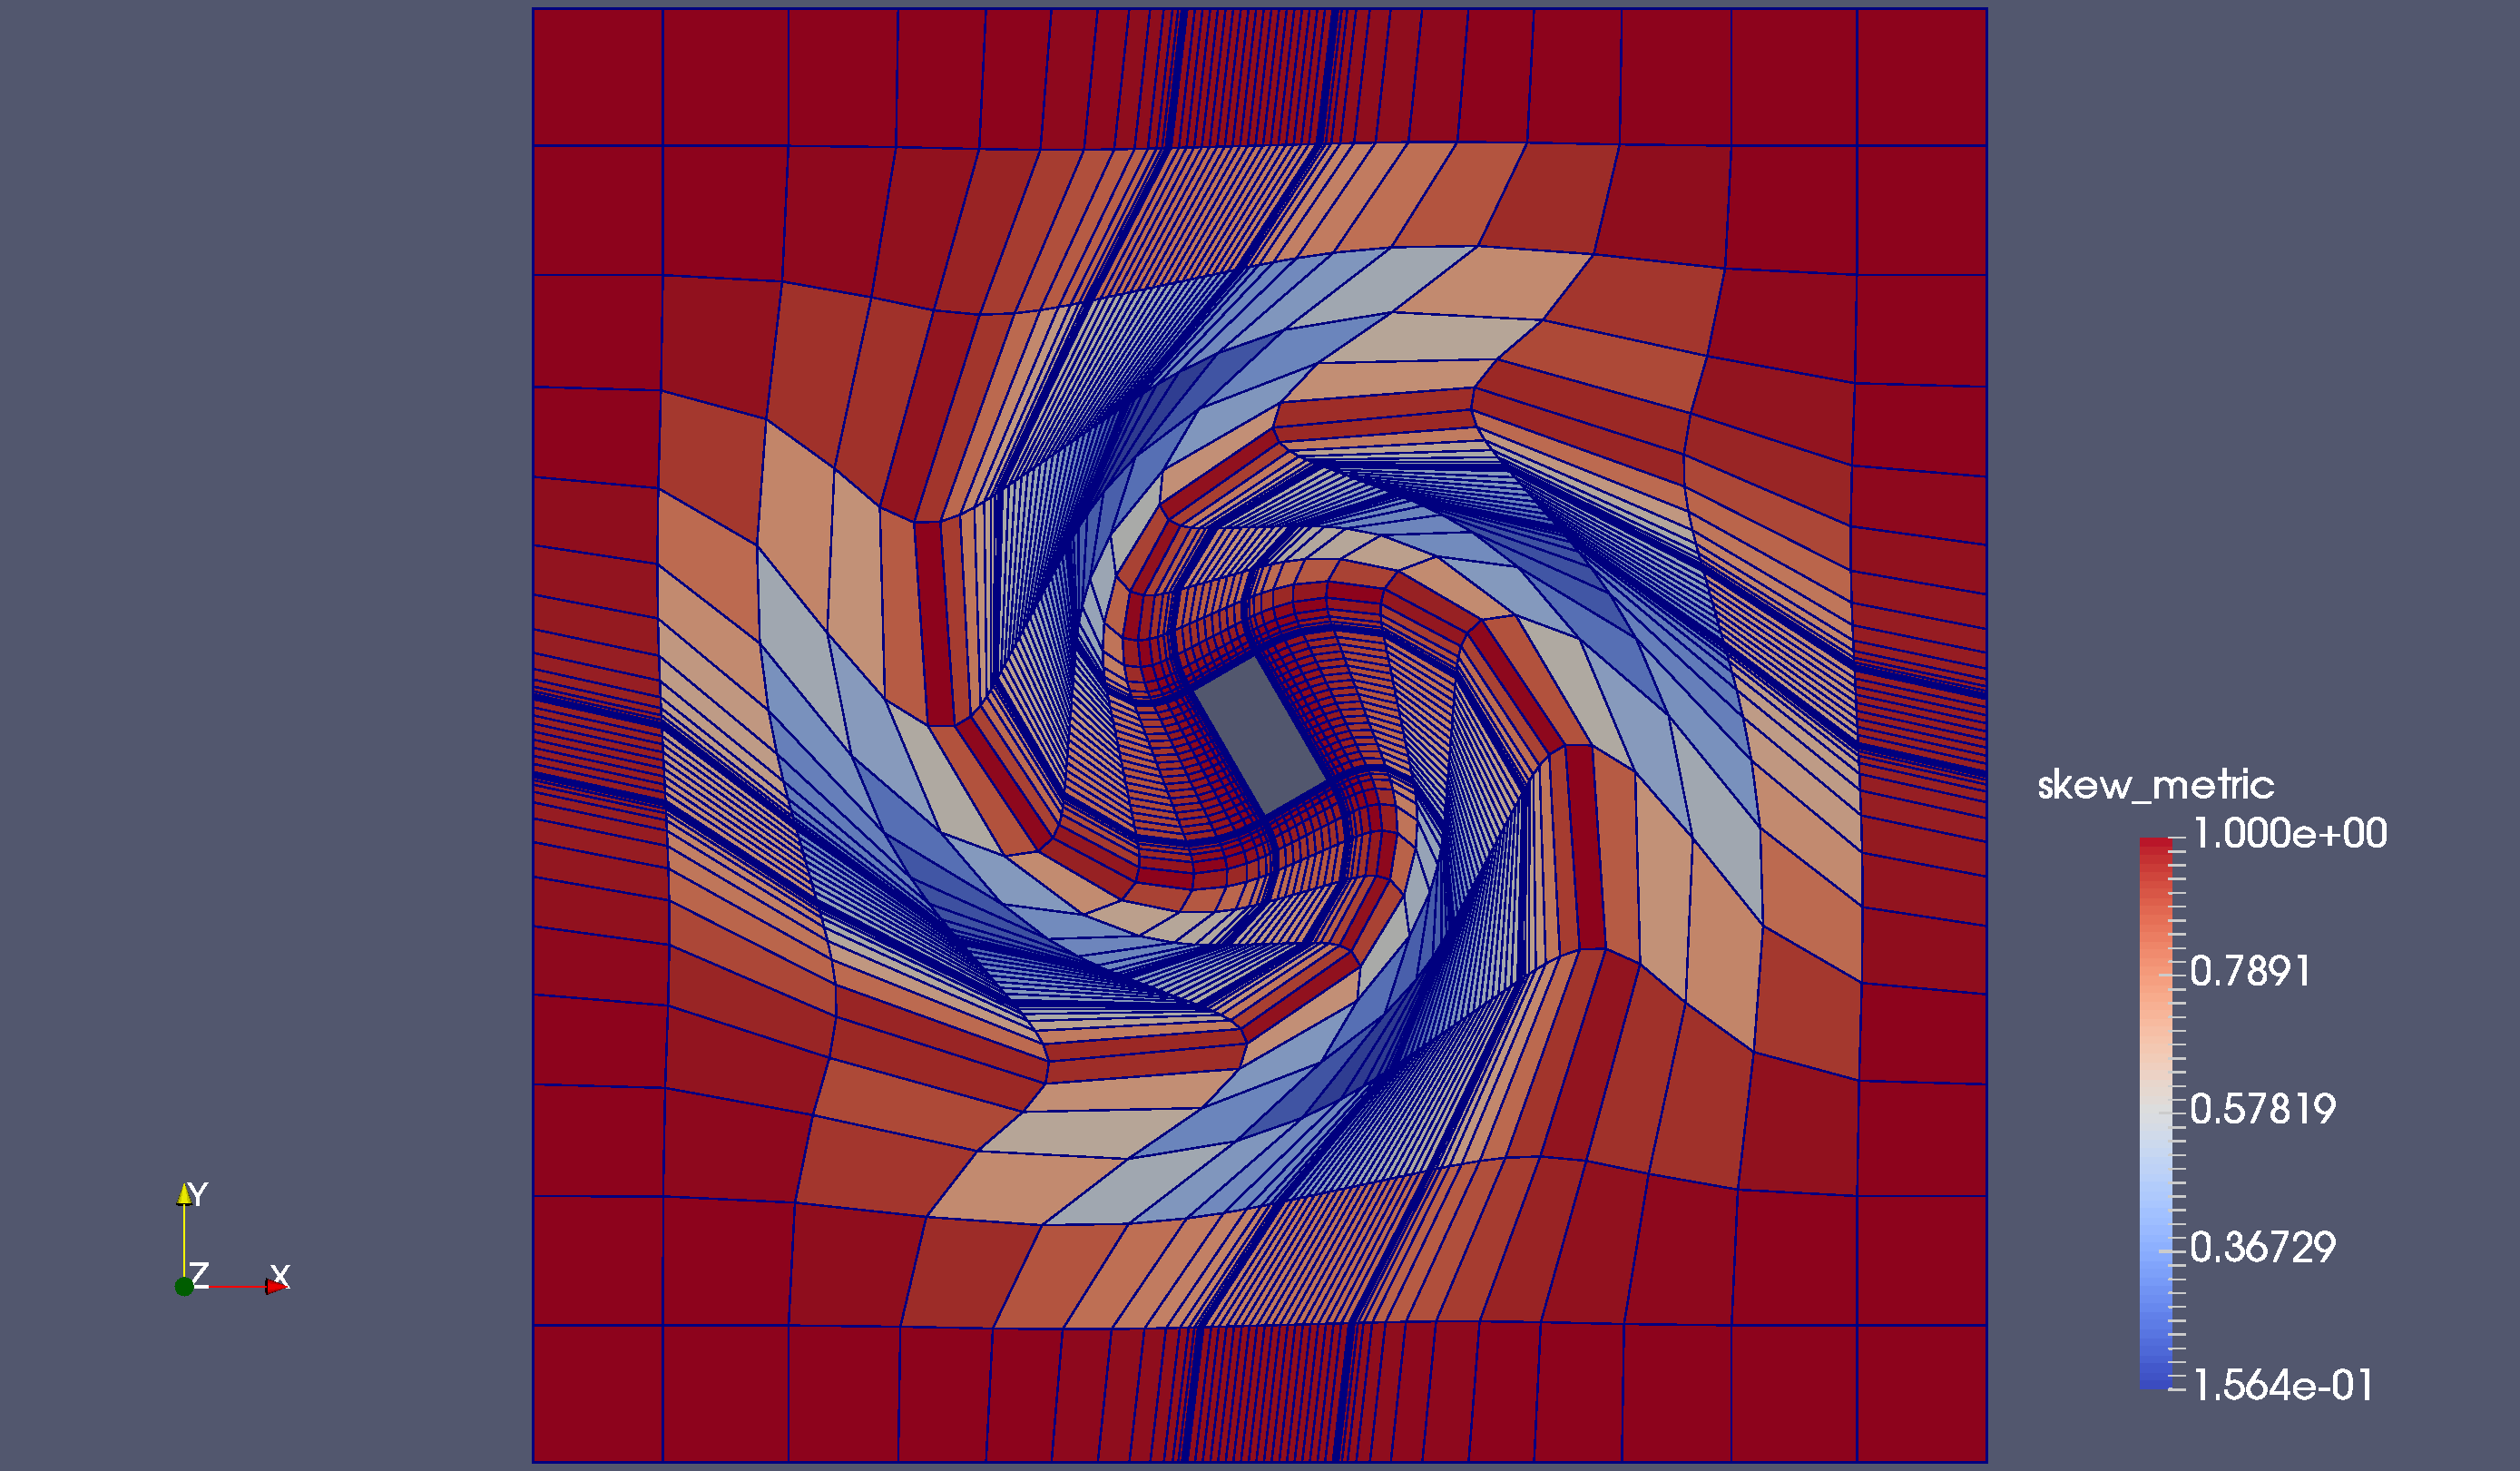
\includegraphics[scale=0.25]{qin-120-quality-withmesh.pdf}
 	\caption{Large rotational motion carried out by DGRBF2}
 	\label{fig:qin-dgrbf2-120}
 \end{figure}
 
 \FloatBarrier
 
 \section{Generation of curved meshes}
 
 Curved meshes for various standard viscous flow test cases have been generated with the method described in the previous section. These include flow past NACA0012 airfoil, flow through a bump channel and flow past a multi-element airfoil. Out of these, the mesh for the multi-element airfoil case is a truly unstructured mesh; the others are structured meshes which we first convert to unstructured format.
 
 The validity and quality of the generated mesh is established by computing the minimum scaled Jacobian determinant for each element. If the minimum value of the Jacobian determinant is zero or negative, the element is considered invalid. This is done as a post-processing step using the plugin `AnalyseCurvedMesh' available in Gmsh \cite{gmsh}. The quantity computed by this plugin is given as
 \begin{equation} 
 m_i = \frac{\inf_{\mathbf{x}\in\Omega_i}\det \mathbf{J}(\mathbf{x})}{\det \mathbf{J_l}_i},
 \end{equation}
 where $\mathbf{J}$ is the Jacobian matrix of the transformation of a reference element to the curved physical element, and $\mathbf{J_l}$ is the Jacobian of the transformation of the reference element to the linear (straight) physical element. $\Omega_i$ represents the \emph{i}th element.
 
 \subsection{2D Viscous Flow Mesh of Multi-element airfoil}
 Here, we present results of 2D curved mesh generation in case of a multi-element airfoil. The mesh has 66530 triangular elements, 133768 total nodes and 1420 boundary nodes. It is meant for viscous flow computations and thus has highly stretched, thin elements near the wing boundaries. In this case, if the interior nodes are not moved properly, invalid elements result. In the figures, we compare curved meshes generated by isotropic linear elasticity and RBF interpolation. Both problems are solved using a point Jacobi preconditioned conjugate gradient solver. Linear elasticity method uses a Young's modulus $E$ of $1\times 10^6$ Pa and a Poisson's ratio of 0.4, though it is observed that different values do not influence the outcome; a number of values over the range 1.0 to $1.0 \times 10^{10}$ were tried for $E$. RBF interpolation uses a support radius of 0.04 (for reference, the chord length of the wing is approximately 18.3).
 
 \begin{figure}
 	\centering
 	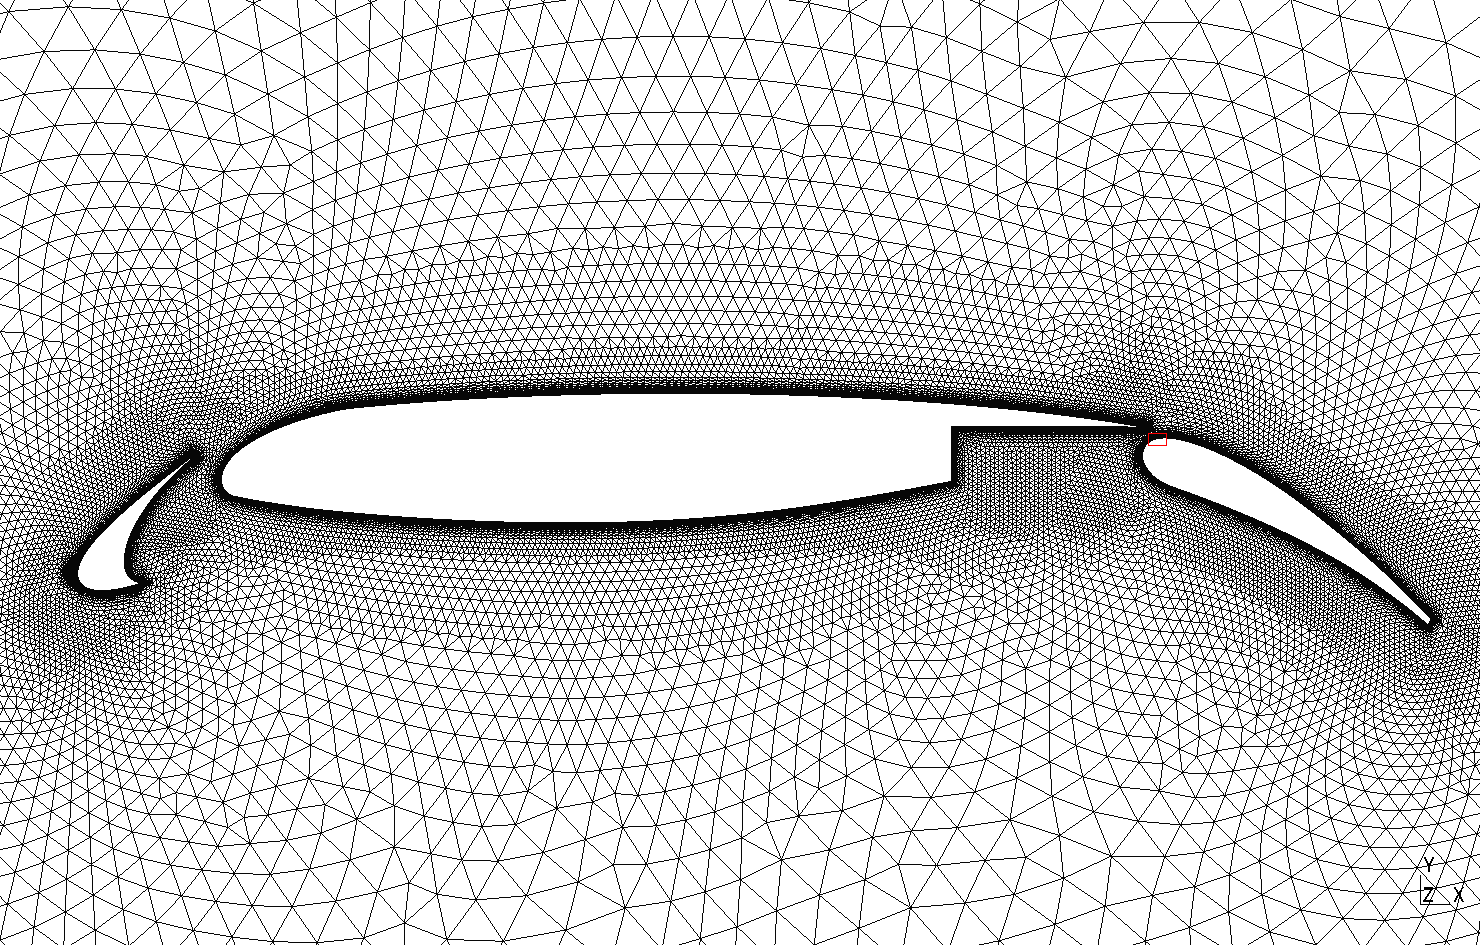
\includegraphics[width=300.0pt]{3compblack}
 	\caption{Mesh of multi-element airfoil. The little box shows approximately the region which is magnified in the figures that follow.}
 \end{figure}
 
% \begin{figure}
% 	\centering
% 	\subfloat{
% 		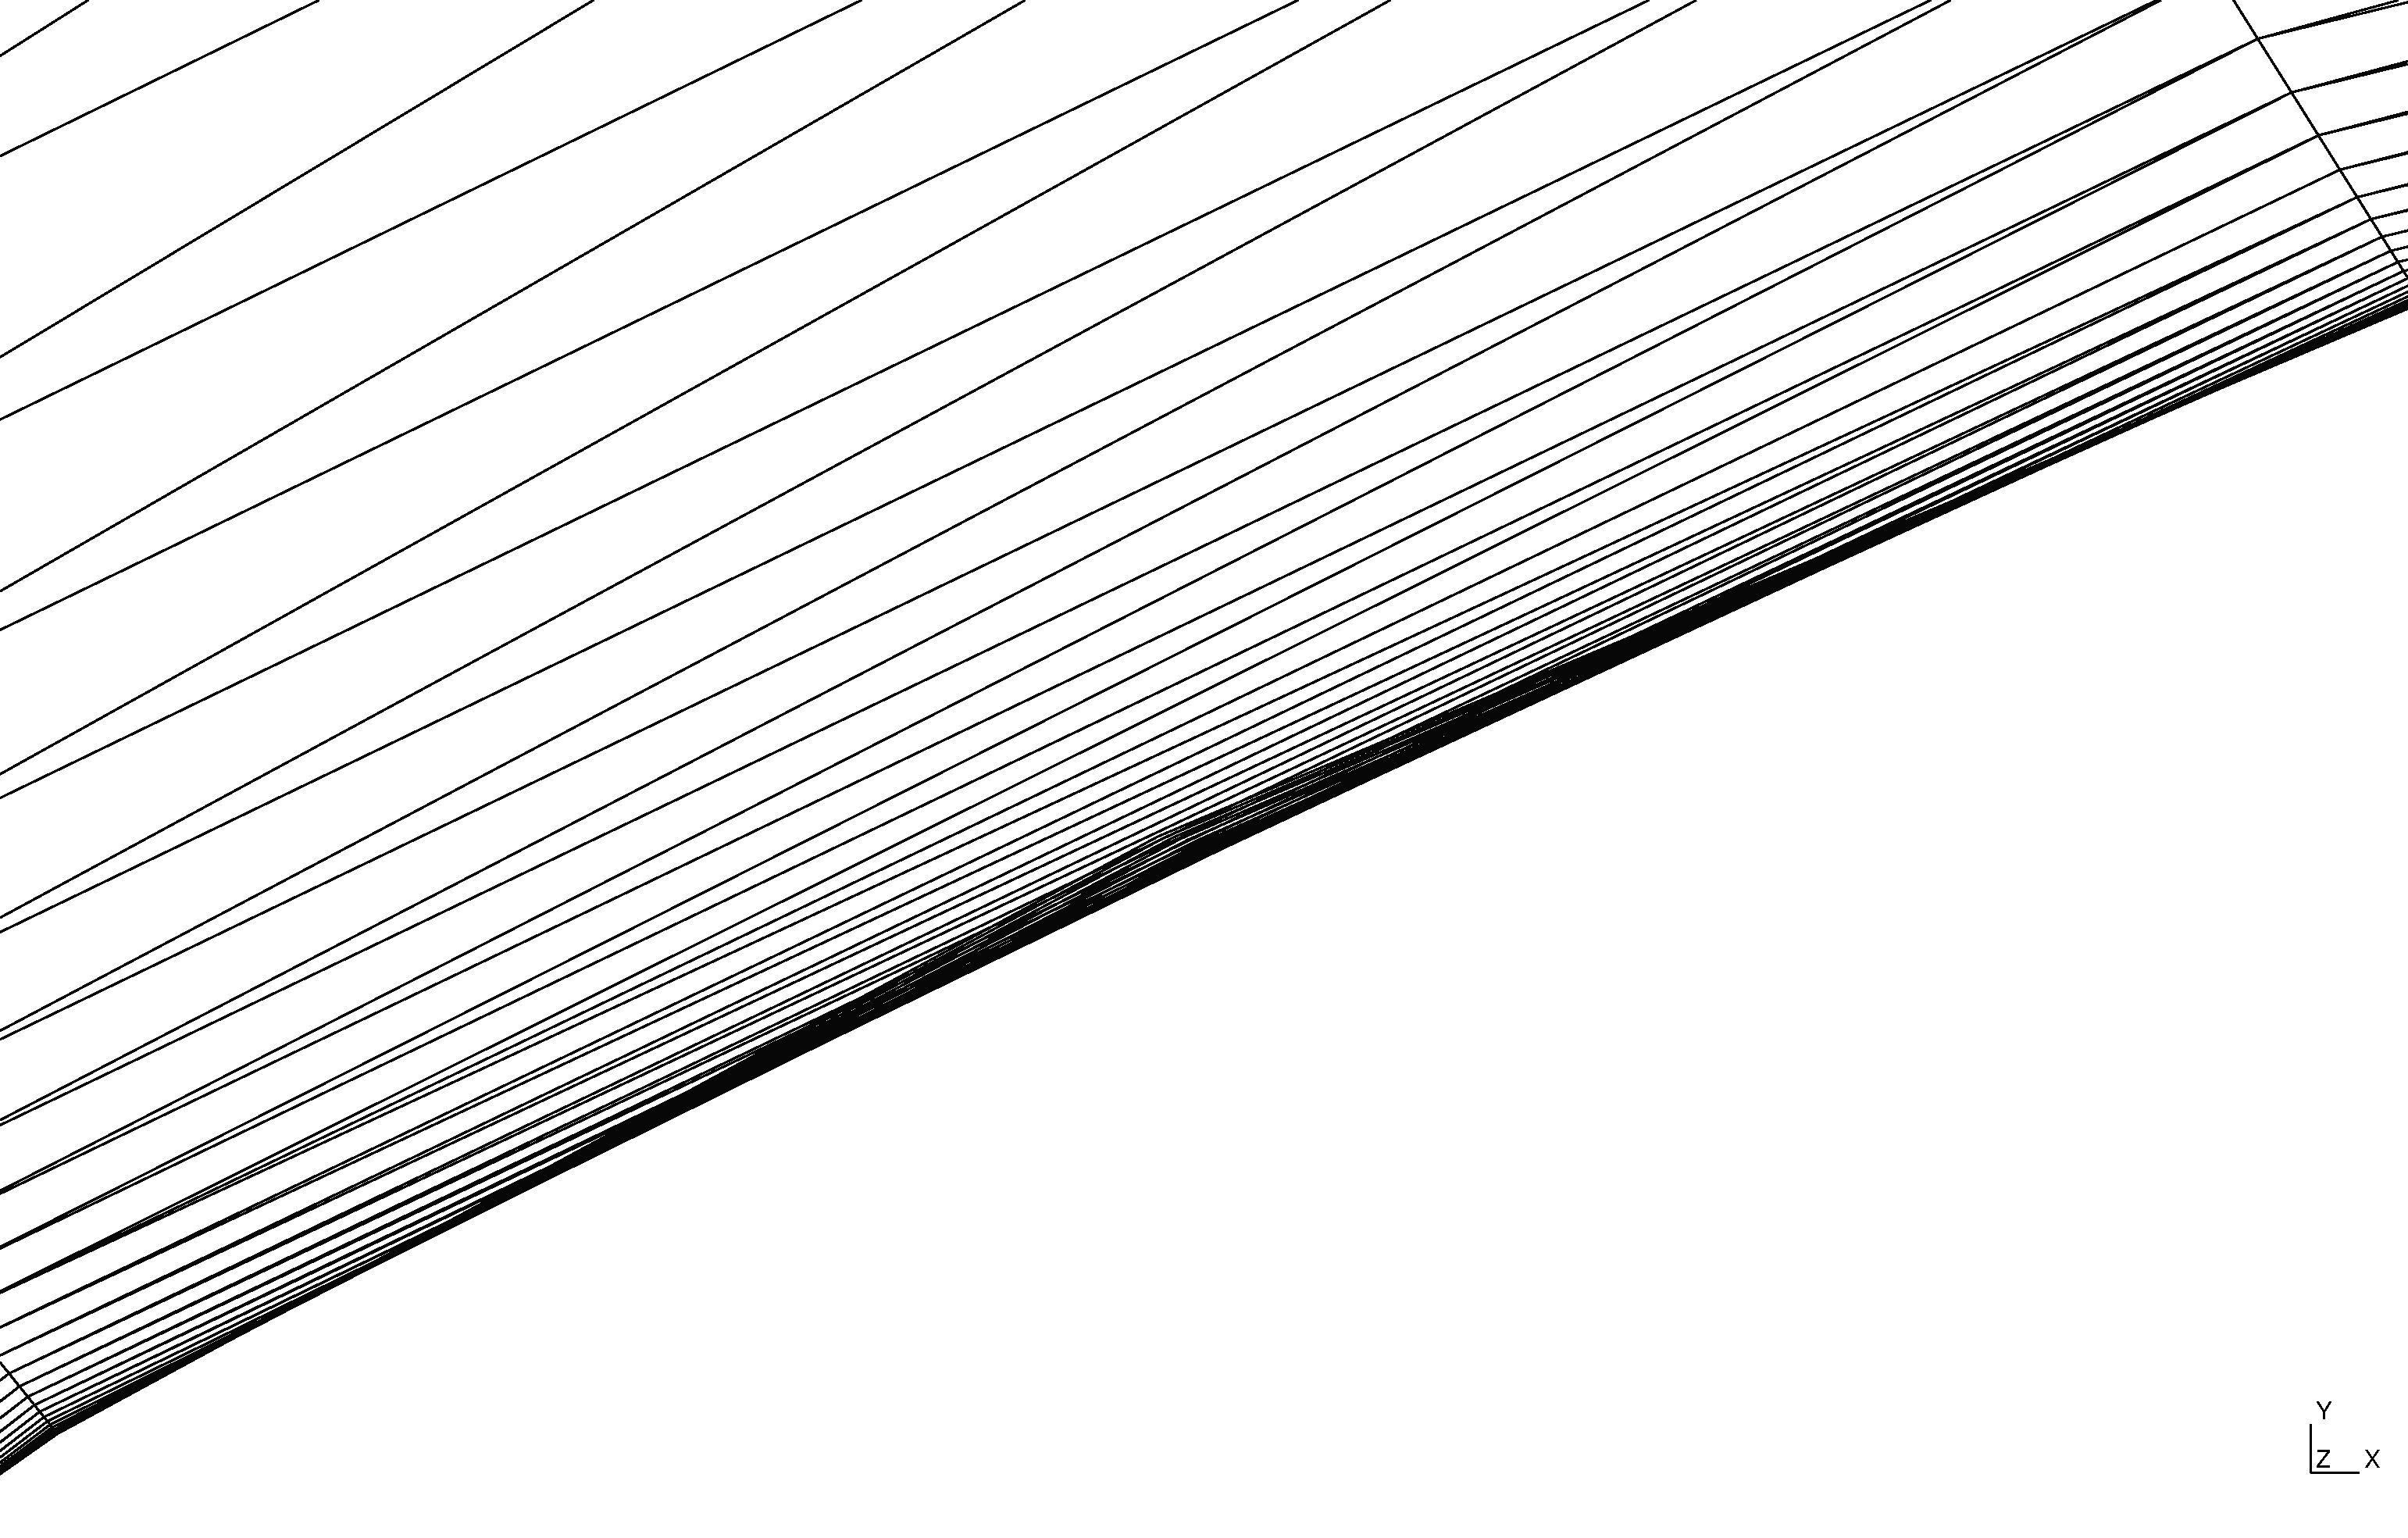
\includegraphics[width=200.0pt]{3comp-elast-zoomedblk.pdf}
% 	}
% 	\subfloat{
% 		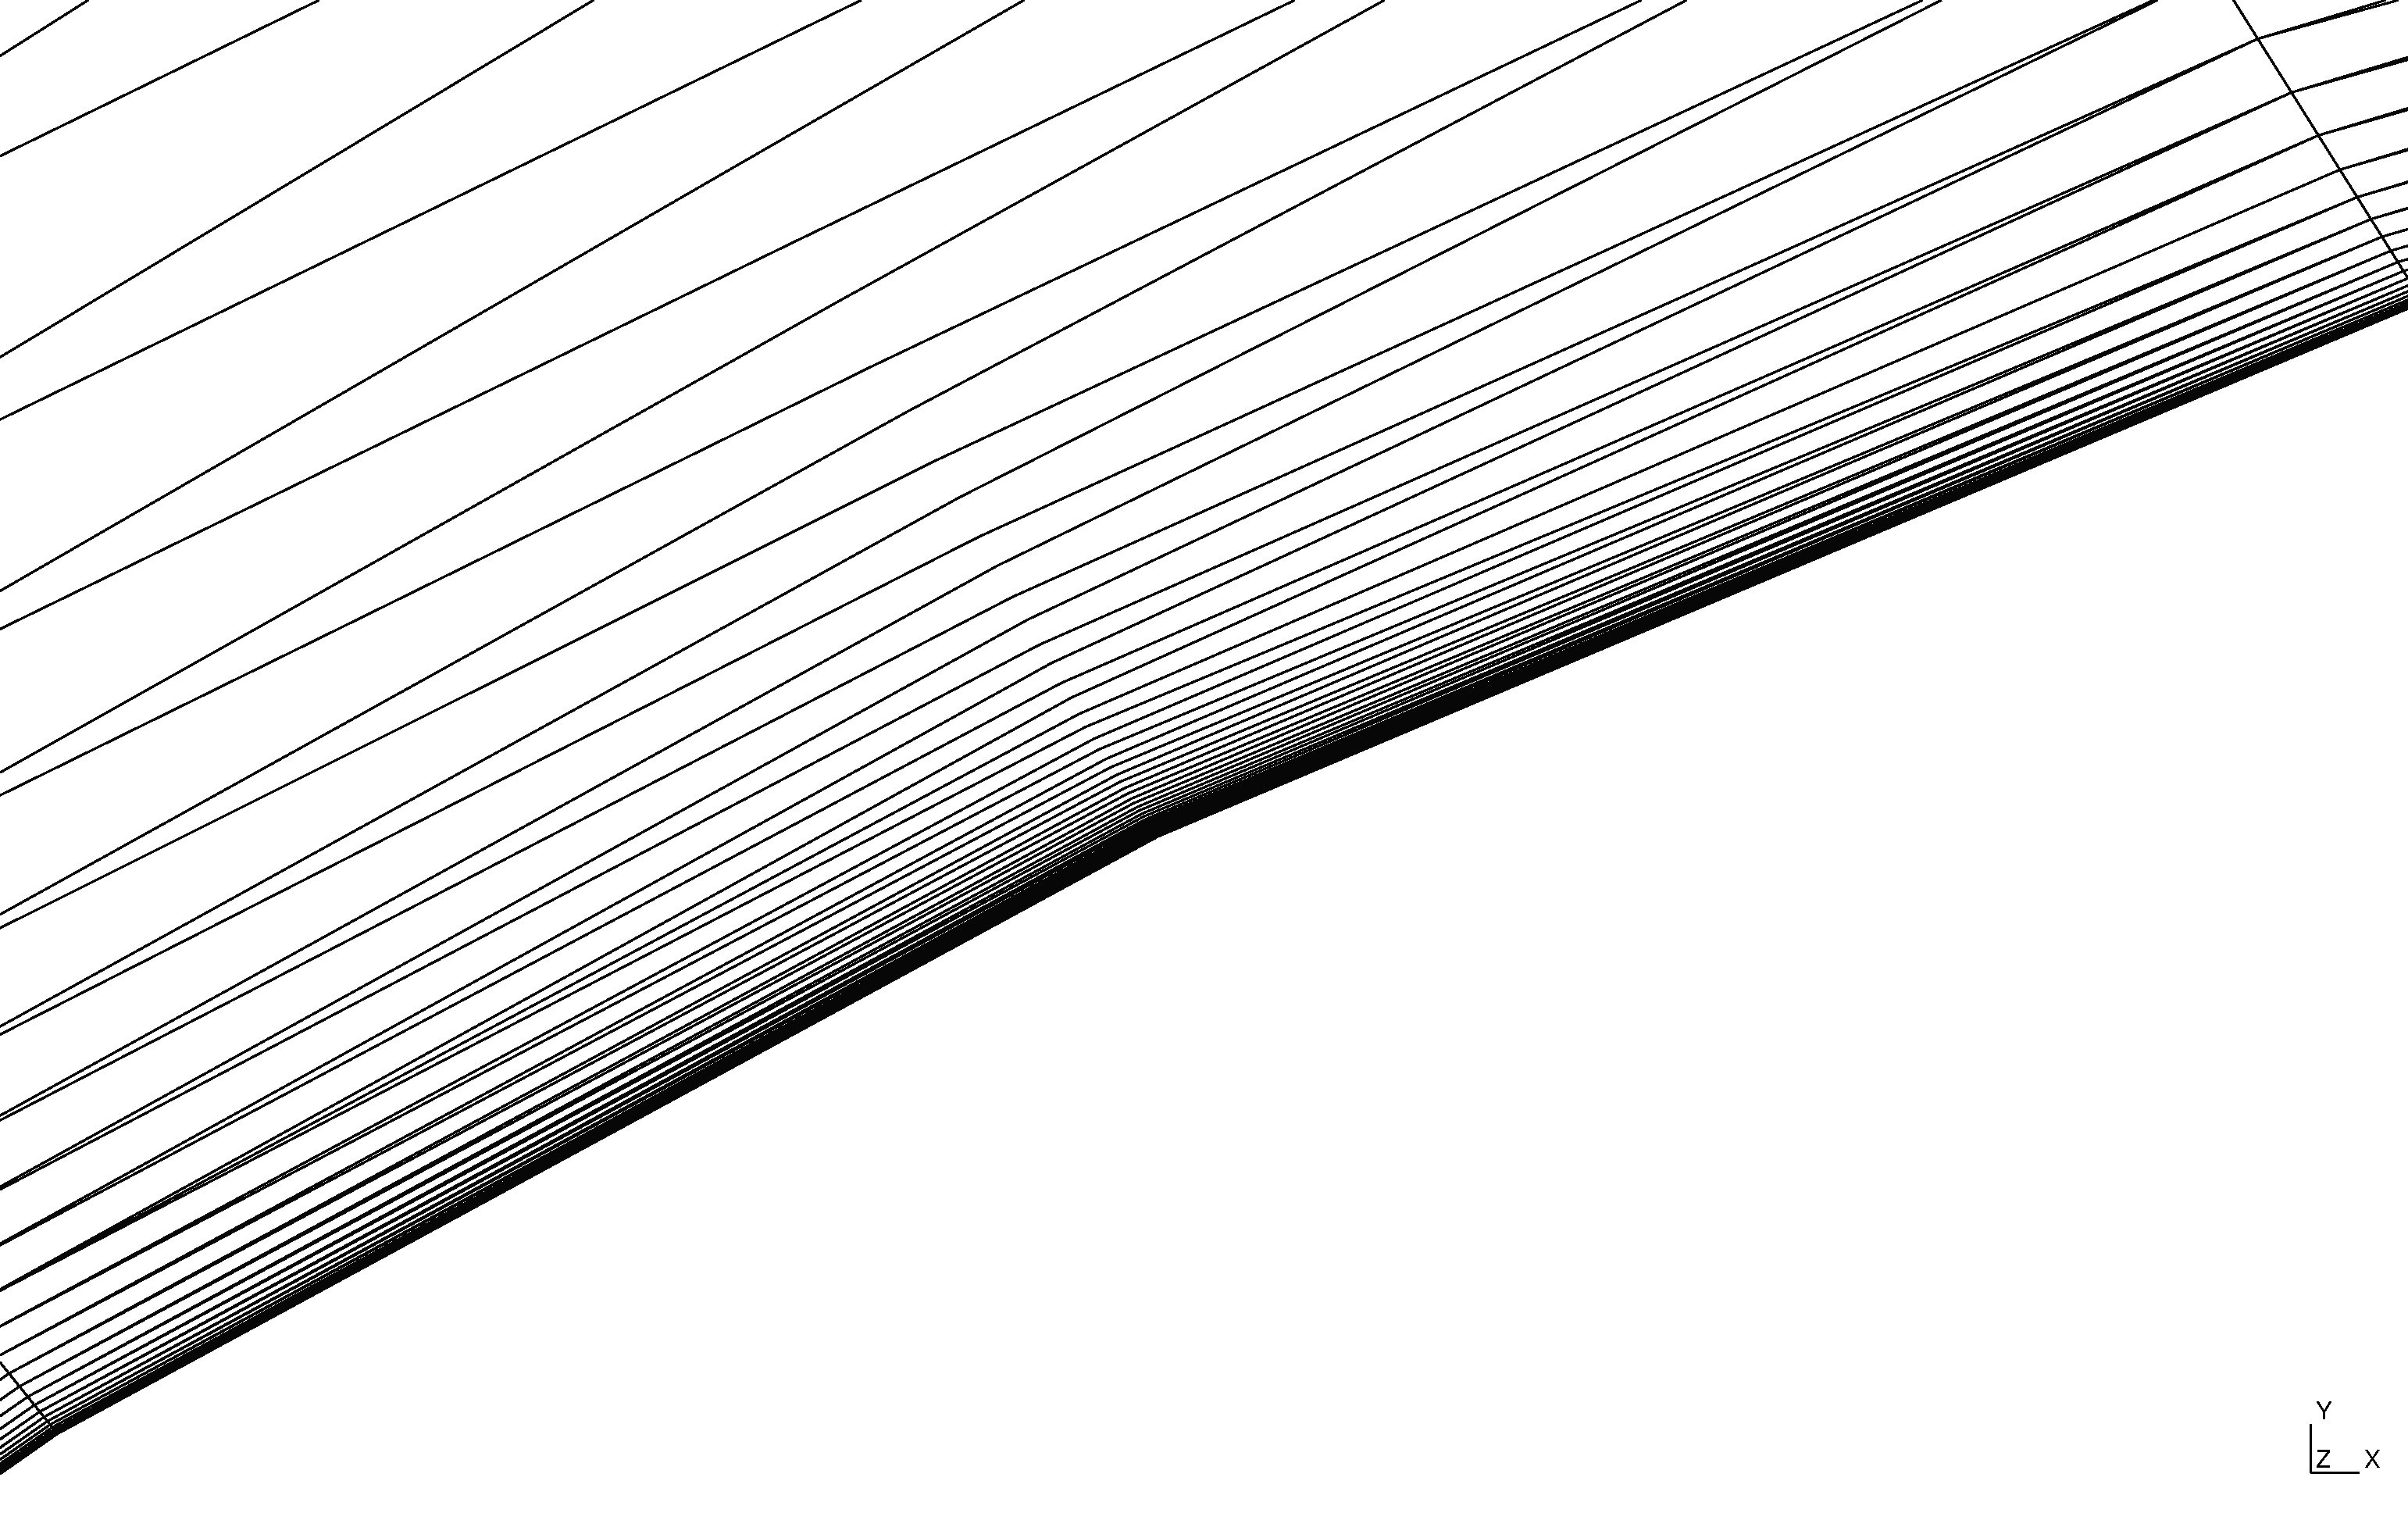
\includegraphics[width=200.0pt]{3comp-rbf-zoomedblk.pdf}
% 	}
% 	\caption{Portion of quadratic viscous mesh for multi-element airfoil, showing a boundary face in the flap, generated by linear elasticity (left) and RBF (right) methods.}
% 	\label{fig:tangled1}
% \end{figure}
 
 \begin{figure}
 	\centering
 	\subfloat{
 		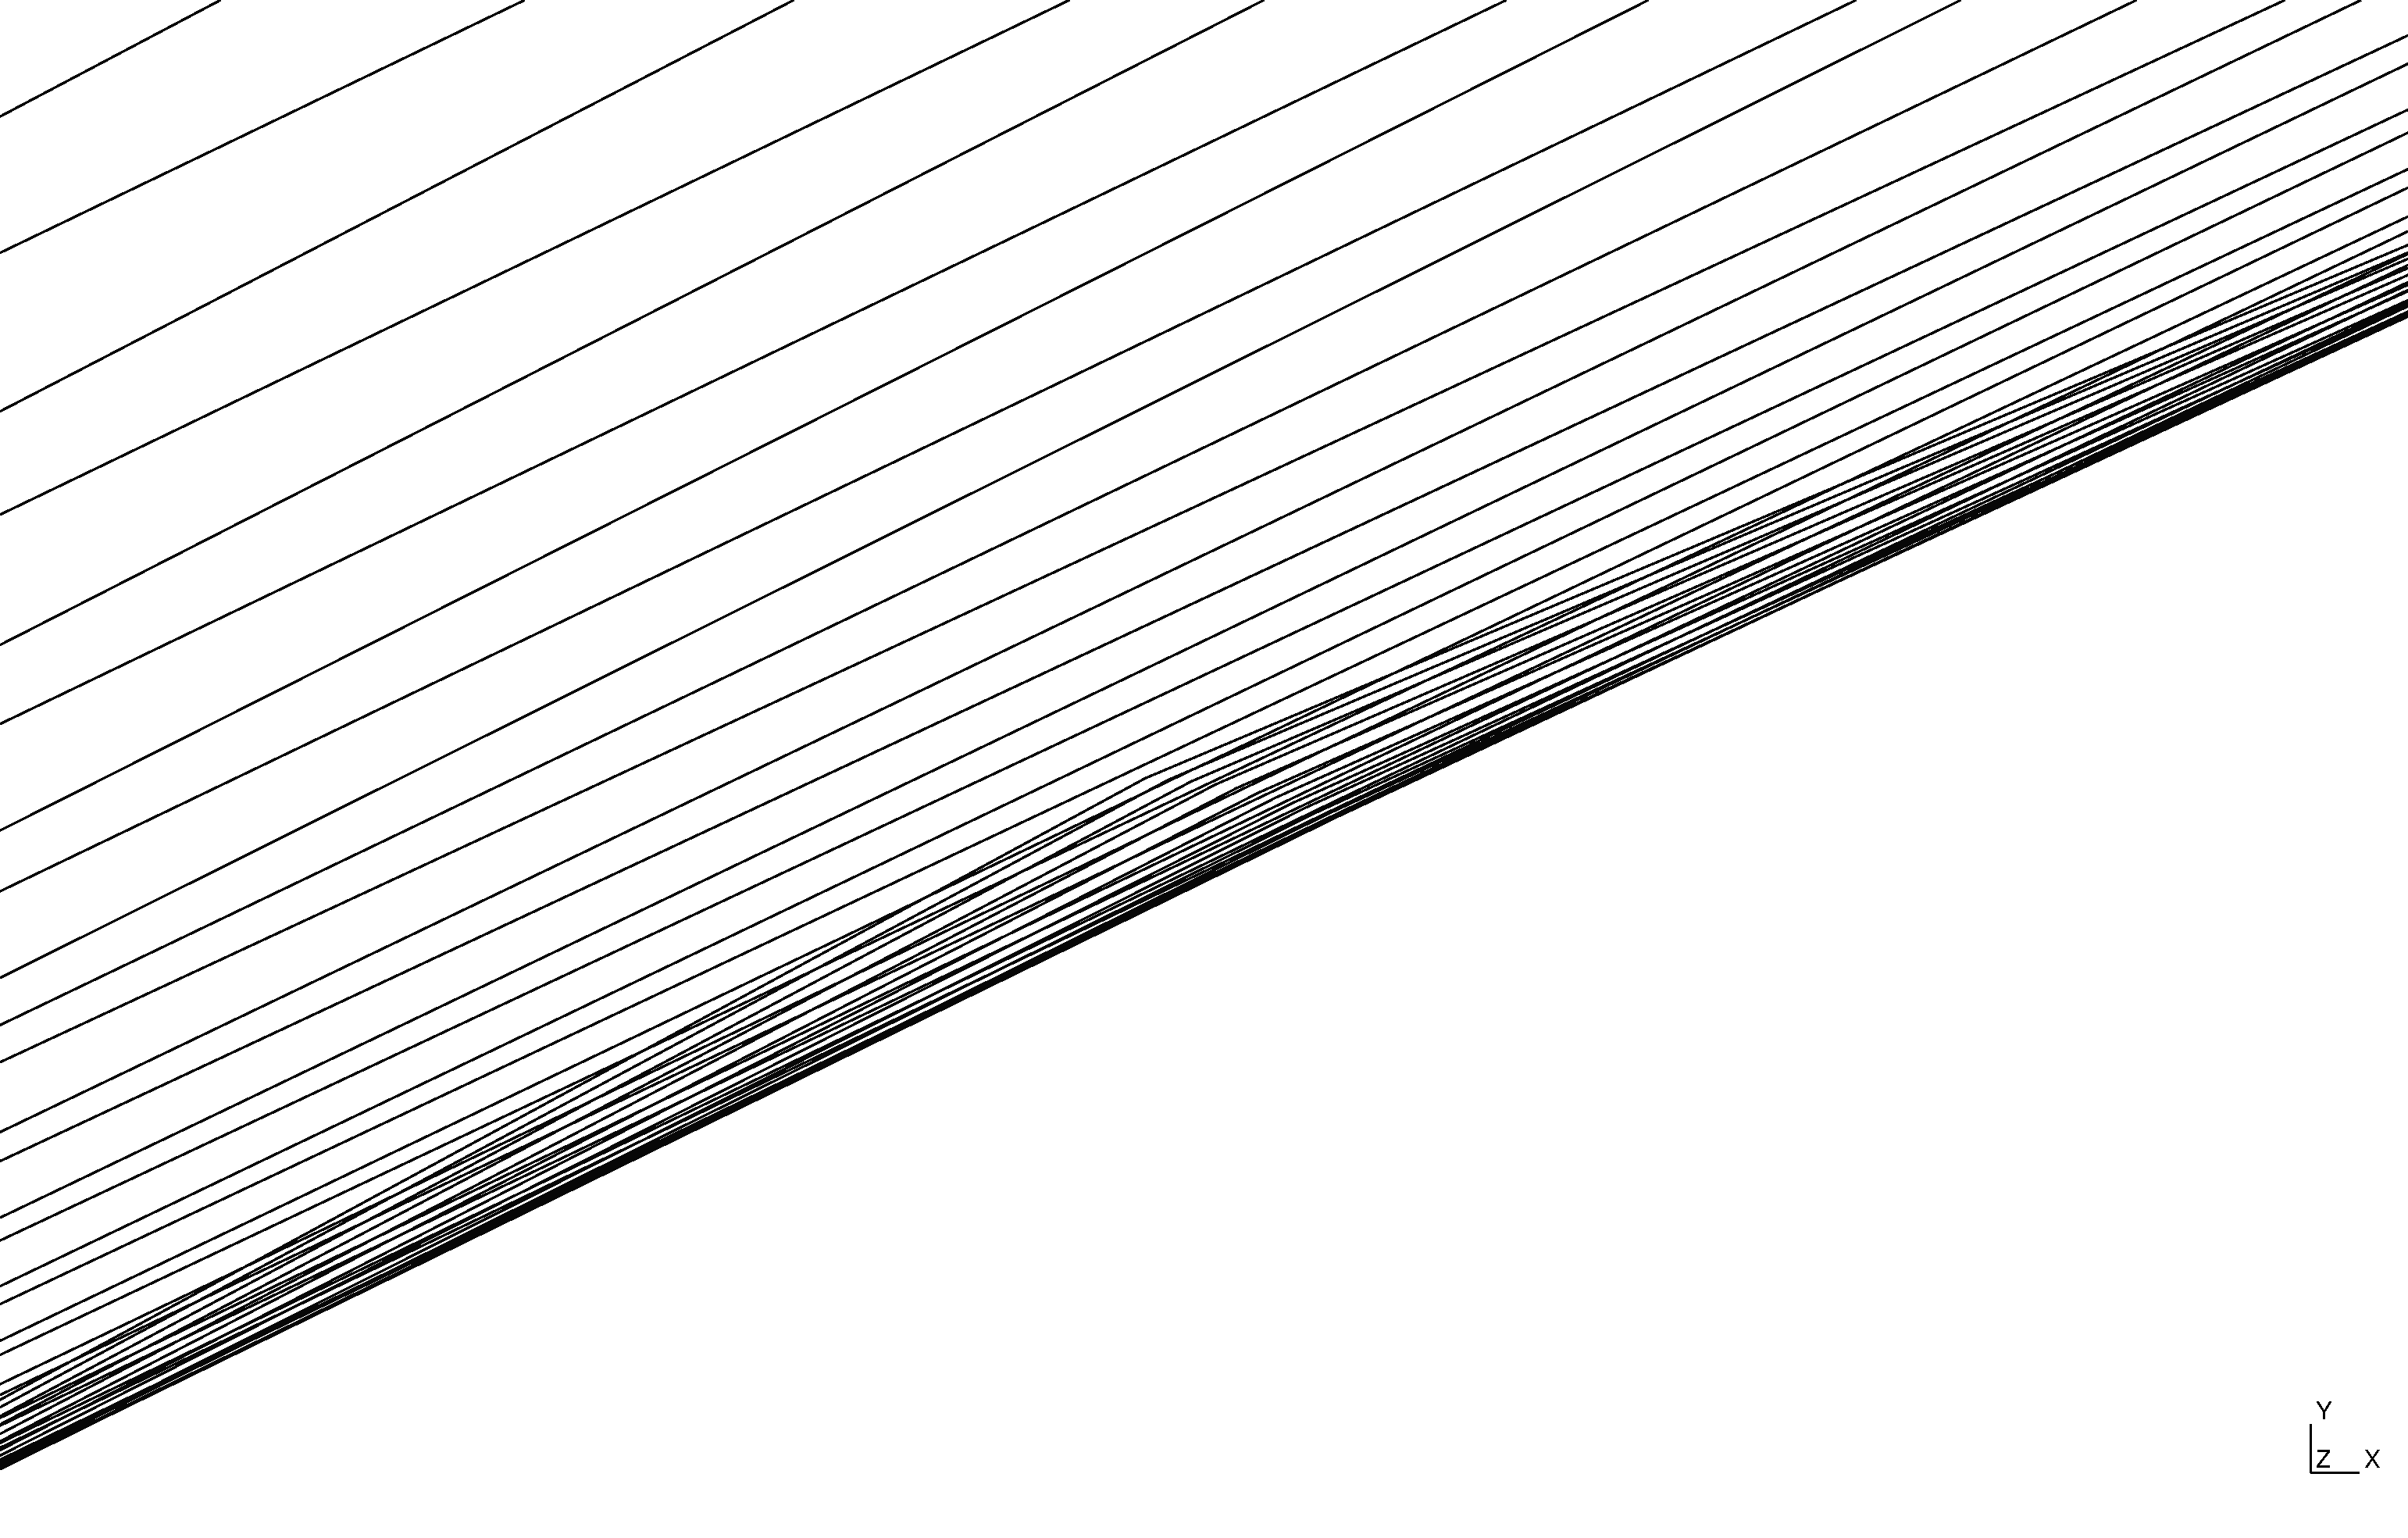
\includegraphics[width=200.0pt]{3comp-elast-vzoomedblk.pdf}
 	}
 	\subfloat{
 		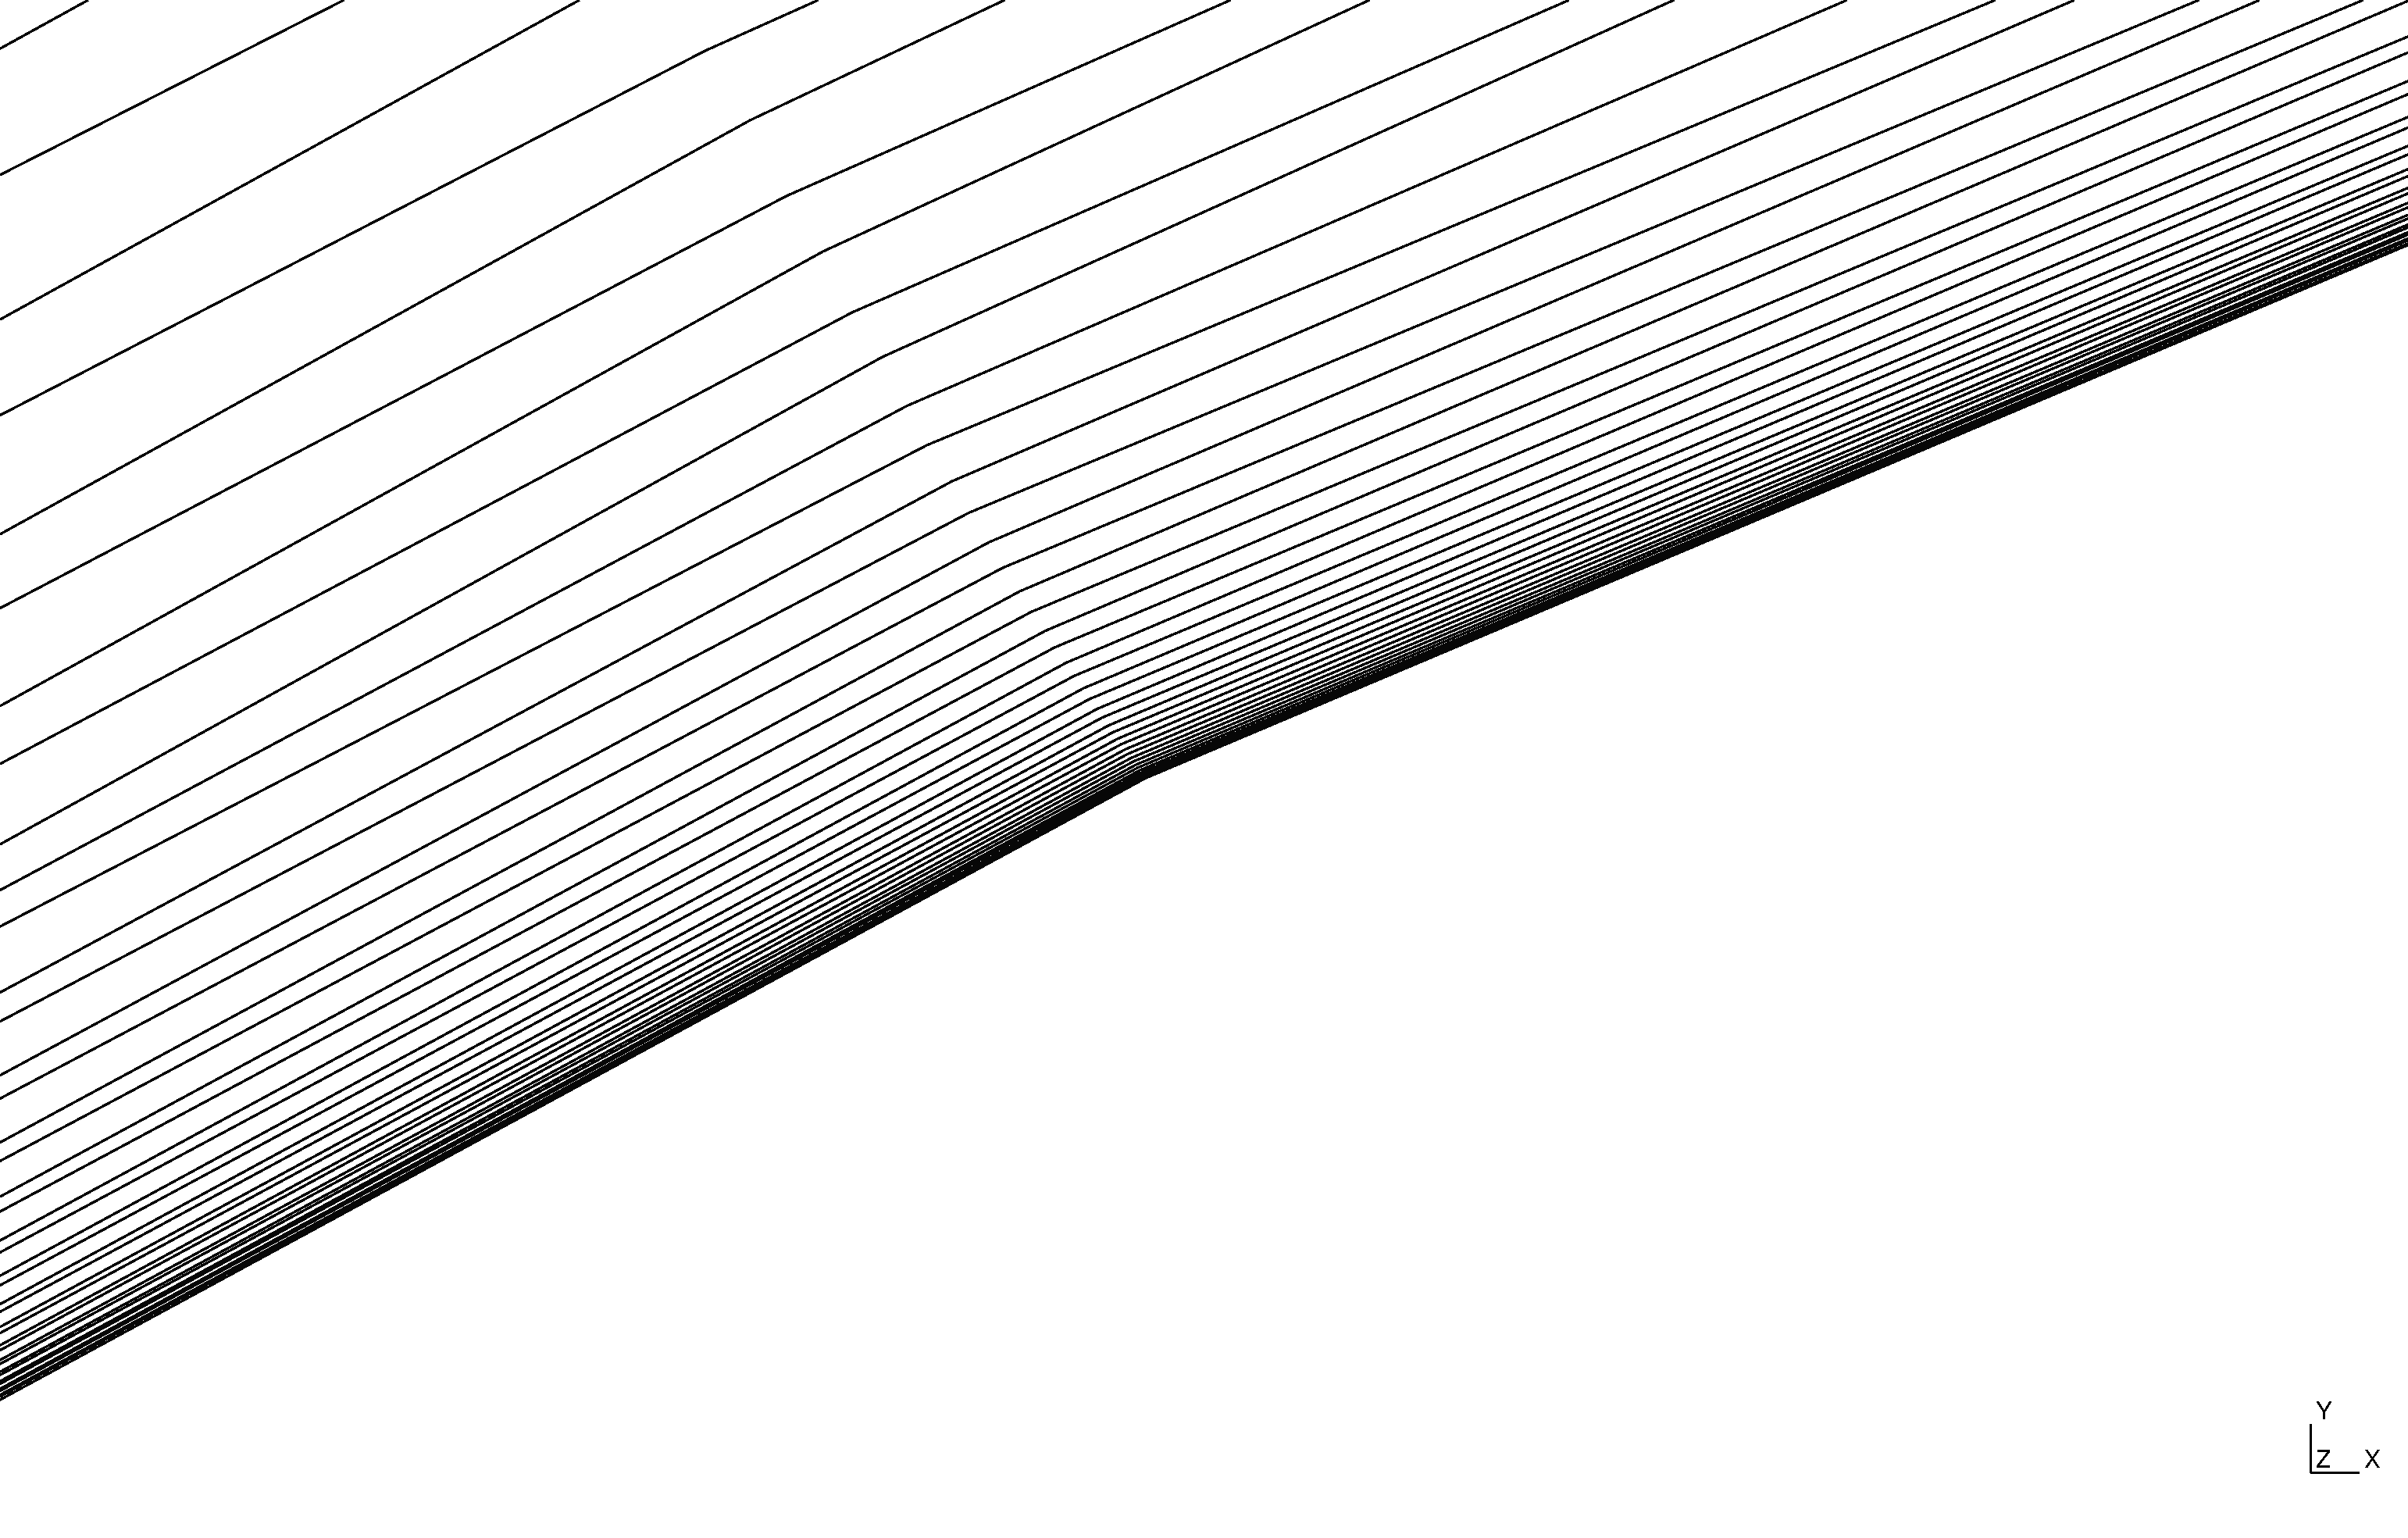
\includegraphics[width=200.0pt]{3comp-rbf-vzoomedblk.pdf}
 	}
 	\caption{Portion of quadratic viscous mesh for multi-element airfoil, showing a boundary face in the flap, generated by linear elasticity (left) and RBF (right) methods. Both are zoomed to for a clearer view.}
 	\label{fig:tangled2}
 \end{figure}
 
 In figure \ref{fig:tangled2}, the first mesh is tangled; even though the nodes are being moved, they are not being moved far enough. It is clear that simple linear elasticity is not enough for curved mesh generation - we get negative Jacobians in several near-boundary elements for many curved boundary faces. However, the RBF method is satisfactory, with a scaled minimum Jacobian range of 0.64 to 1.0 throughout the mesh (figure \ref{fig:rbf-jacobians}). As explained earlier, we see that the elements very close to the boundary deform very little - they have scaled Jacobian nearly 1.0. As we go further from the boundary, the Jacobian drops to a minimum and then rises again to 1.0 at a distance that approximately equals the support radius.
 
 \begin{figure}
 	\centering
 	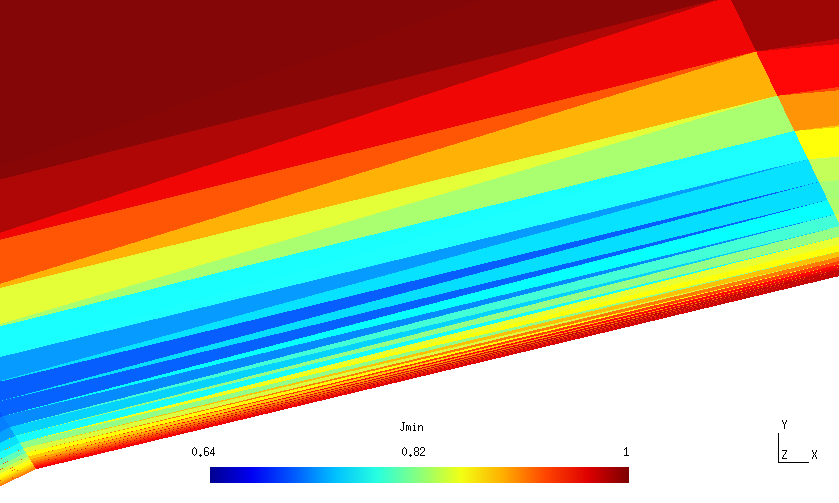
\includegraphics[width=400pt,scale=0.5]{3comp-rbf-zoomed-jacobians2.png}
 	\caption{Minimum scaled Jacobian over each element for mesh generated by RBF interpolation. (The mesh is actually curved, though the graphics of Gmsh ignore that.)}
 	\label{fig:rbf-jacobians}
 \end{figure}

Next, we present results of the same case, but using Jacobian-based stiffening in the linear elasticity formulation. In table \ref{tab:rbfelast} we compare RBF and stiffened linear elasticity; all cases are solved using point-Jacobi preconditioned conjugate gradient solver with a tolerance of $1\times 10^{-6}$.

It is immediately clear that RBF vastly outperforms SLE for curved mesh generation while results of both methods for this case are largely equally good. One interesting characteristic of SLE is that the CG solver takes more and more iterations to converge with increase in the stiffening exponent $\chi$. Therefore, we conclude that the stiffness matrix seems to get more and more ill-conditioned with increase in the stiffening exponent $\chi$, while not providing much improvement in mesh quality. As far as RBF is concerned, we see that increasing the number of steps is not worth the additional time consumed by the solver. Further, it is interesting to note that an increase in support radius beyond a value degrades the mesh quality; there is/are optimum value(s) of the support radius, less than and more than which the mesh quality drops.

\begin{figure}
 	\centering
 	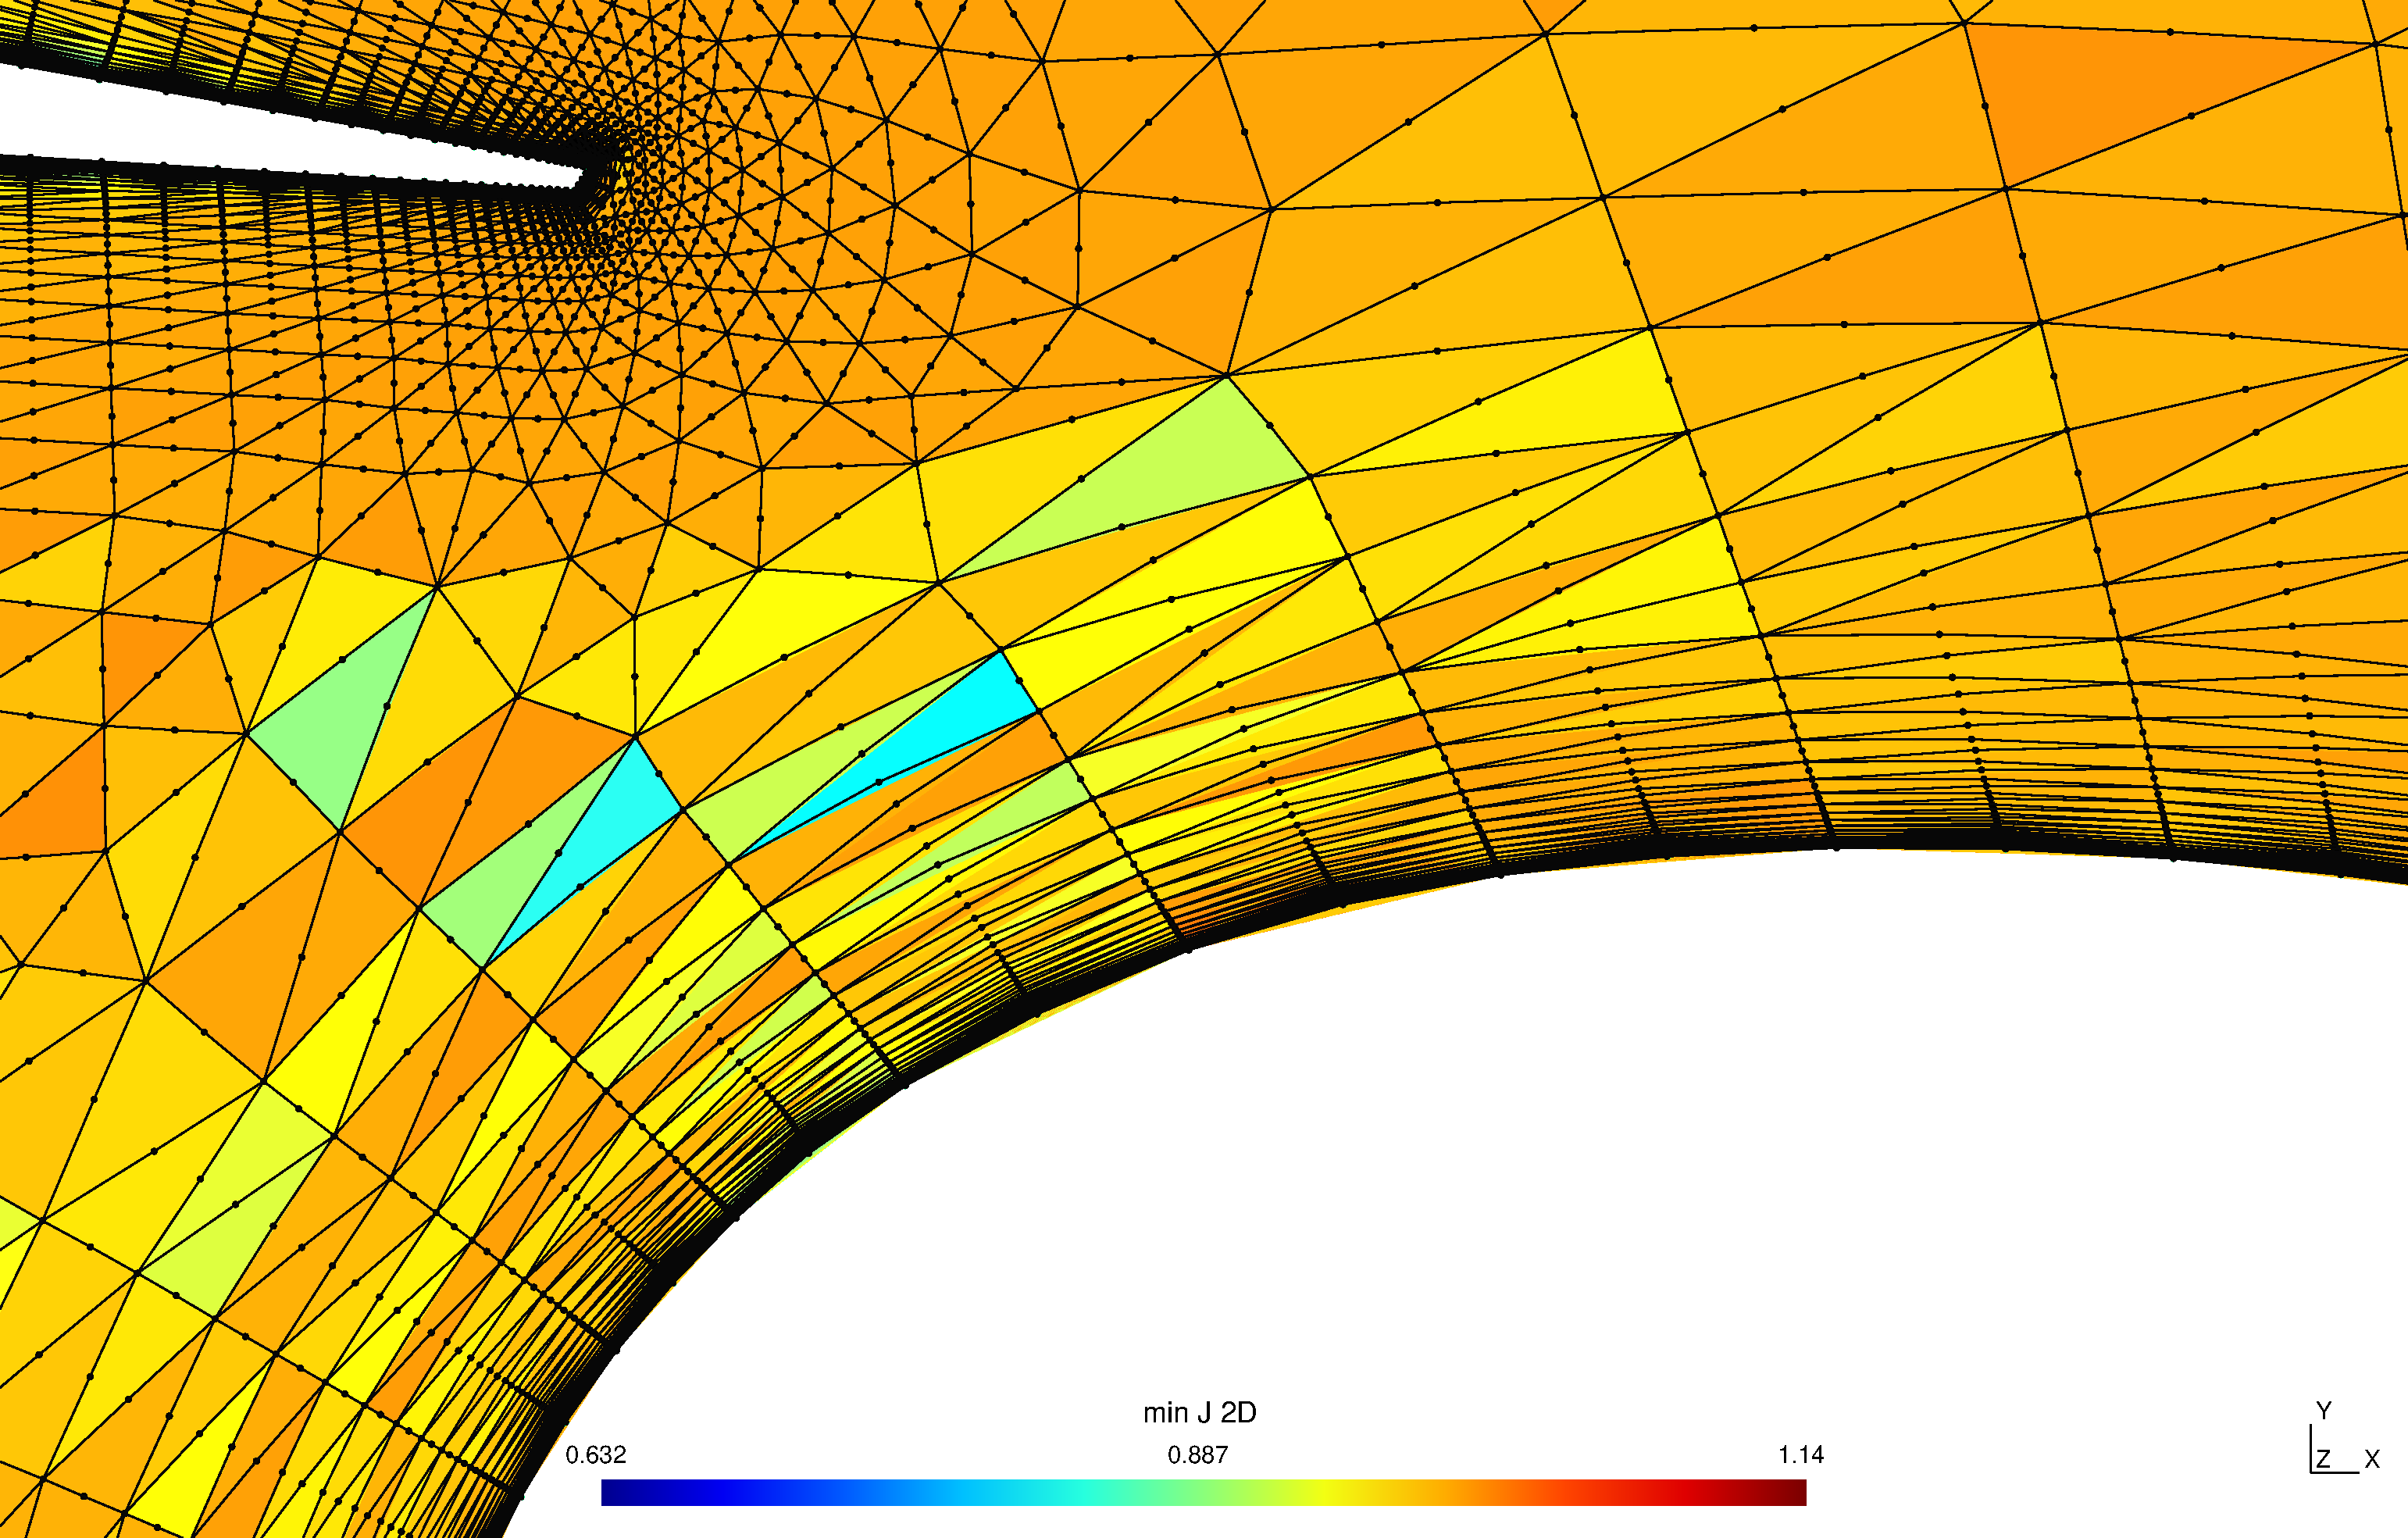
\includegraphics[width=400pt,scale=0.5]{3comp-stiffelast-zoomed}
 	\caption{An illustrative example of a curved mesh generated by stiffened elasticity method; minimum scaled Jacobian over each element is shown}
 	\label{fig:3compstiffelast}
\end{figure}

\begin{table}
\begin{tabular}{|c|c|c|c|c|}
\hline
 Method & Parameters & Minimum scaled Jacobian & Wall clock time & Solver iterations \\
 \hline
\multirow{2}{0.5in}{SLE} & $\chi=2.75$ & 0.632 & 19.3s & 324 \\
				 & $\chi=2.9$ & 0.632 & 24.4s & 423 \\
\multirow{3}{0.5in}{RBF} & 1-step $r_s=0.04$ & 0.640 & 1.86s & 365 x 2 \\
				&   1-step $r_s=0.08$ & 0.639 & 1.9s & 1150 x 2\\
				&   2-step $r_s=0.04$ & 0.641 & 2.58s & 365 x 4\\
\hline
\end{tabular}
\caption{Comparison of RBF (radial basis function) and SLE (stiffened linear elasticity) methods}
\label{tab:rbfelast}
\end{table}
 
\FloatBarrier

\subsection{3D Viscous Flow Mesh for 3D Bump}
This is a Reynolds-averaged Navier-Stokes (RANS) flow simulation test case from the NASA Turbulence models website \cite{case:bump3d}. The simulation parameters include a reference domain length scale of 1.0, Mach number 0.2, Reynolds number of $3\times 10^6$, and a  maximum bump height of 0.05.

For this case, boundary displacements were first obtained from the analytical expression for the bump given on the website. Then, RBF method was used to regularize the interior mesh using Wendland's C2 function. It is notable that this one of the cases where a conjugate gradient solver cannot solve the RBF system. We use a sparse LU decomposition from the Eigen3 C++ library \cite{eigenweb}.

\begin{table}[!h]
\centering
\begin{tabular}{|c|c|c|c|}
	\hline
	  & Coarse & Medium & Fine \\
	 \hline
	 No. of points 				& 32841 & 243729	& 1875489 \\
	 No. of boundary points		& 2304	& 8704		& 33792 \\
	 Support radius				& 0.06	& 0.06		& 0.04 \\
	 Minimum scaled Jacobian	& 0.714	& 0.852		& 0.926 \\
	 Wall-clock time			& 0.68s	& 12.6s		& 338s \\
	 \hline
\end{tabular}
\caption{Summary of 3D bump curved mesh generation}
\end{table}

\begin{figure}
 \centering
 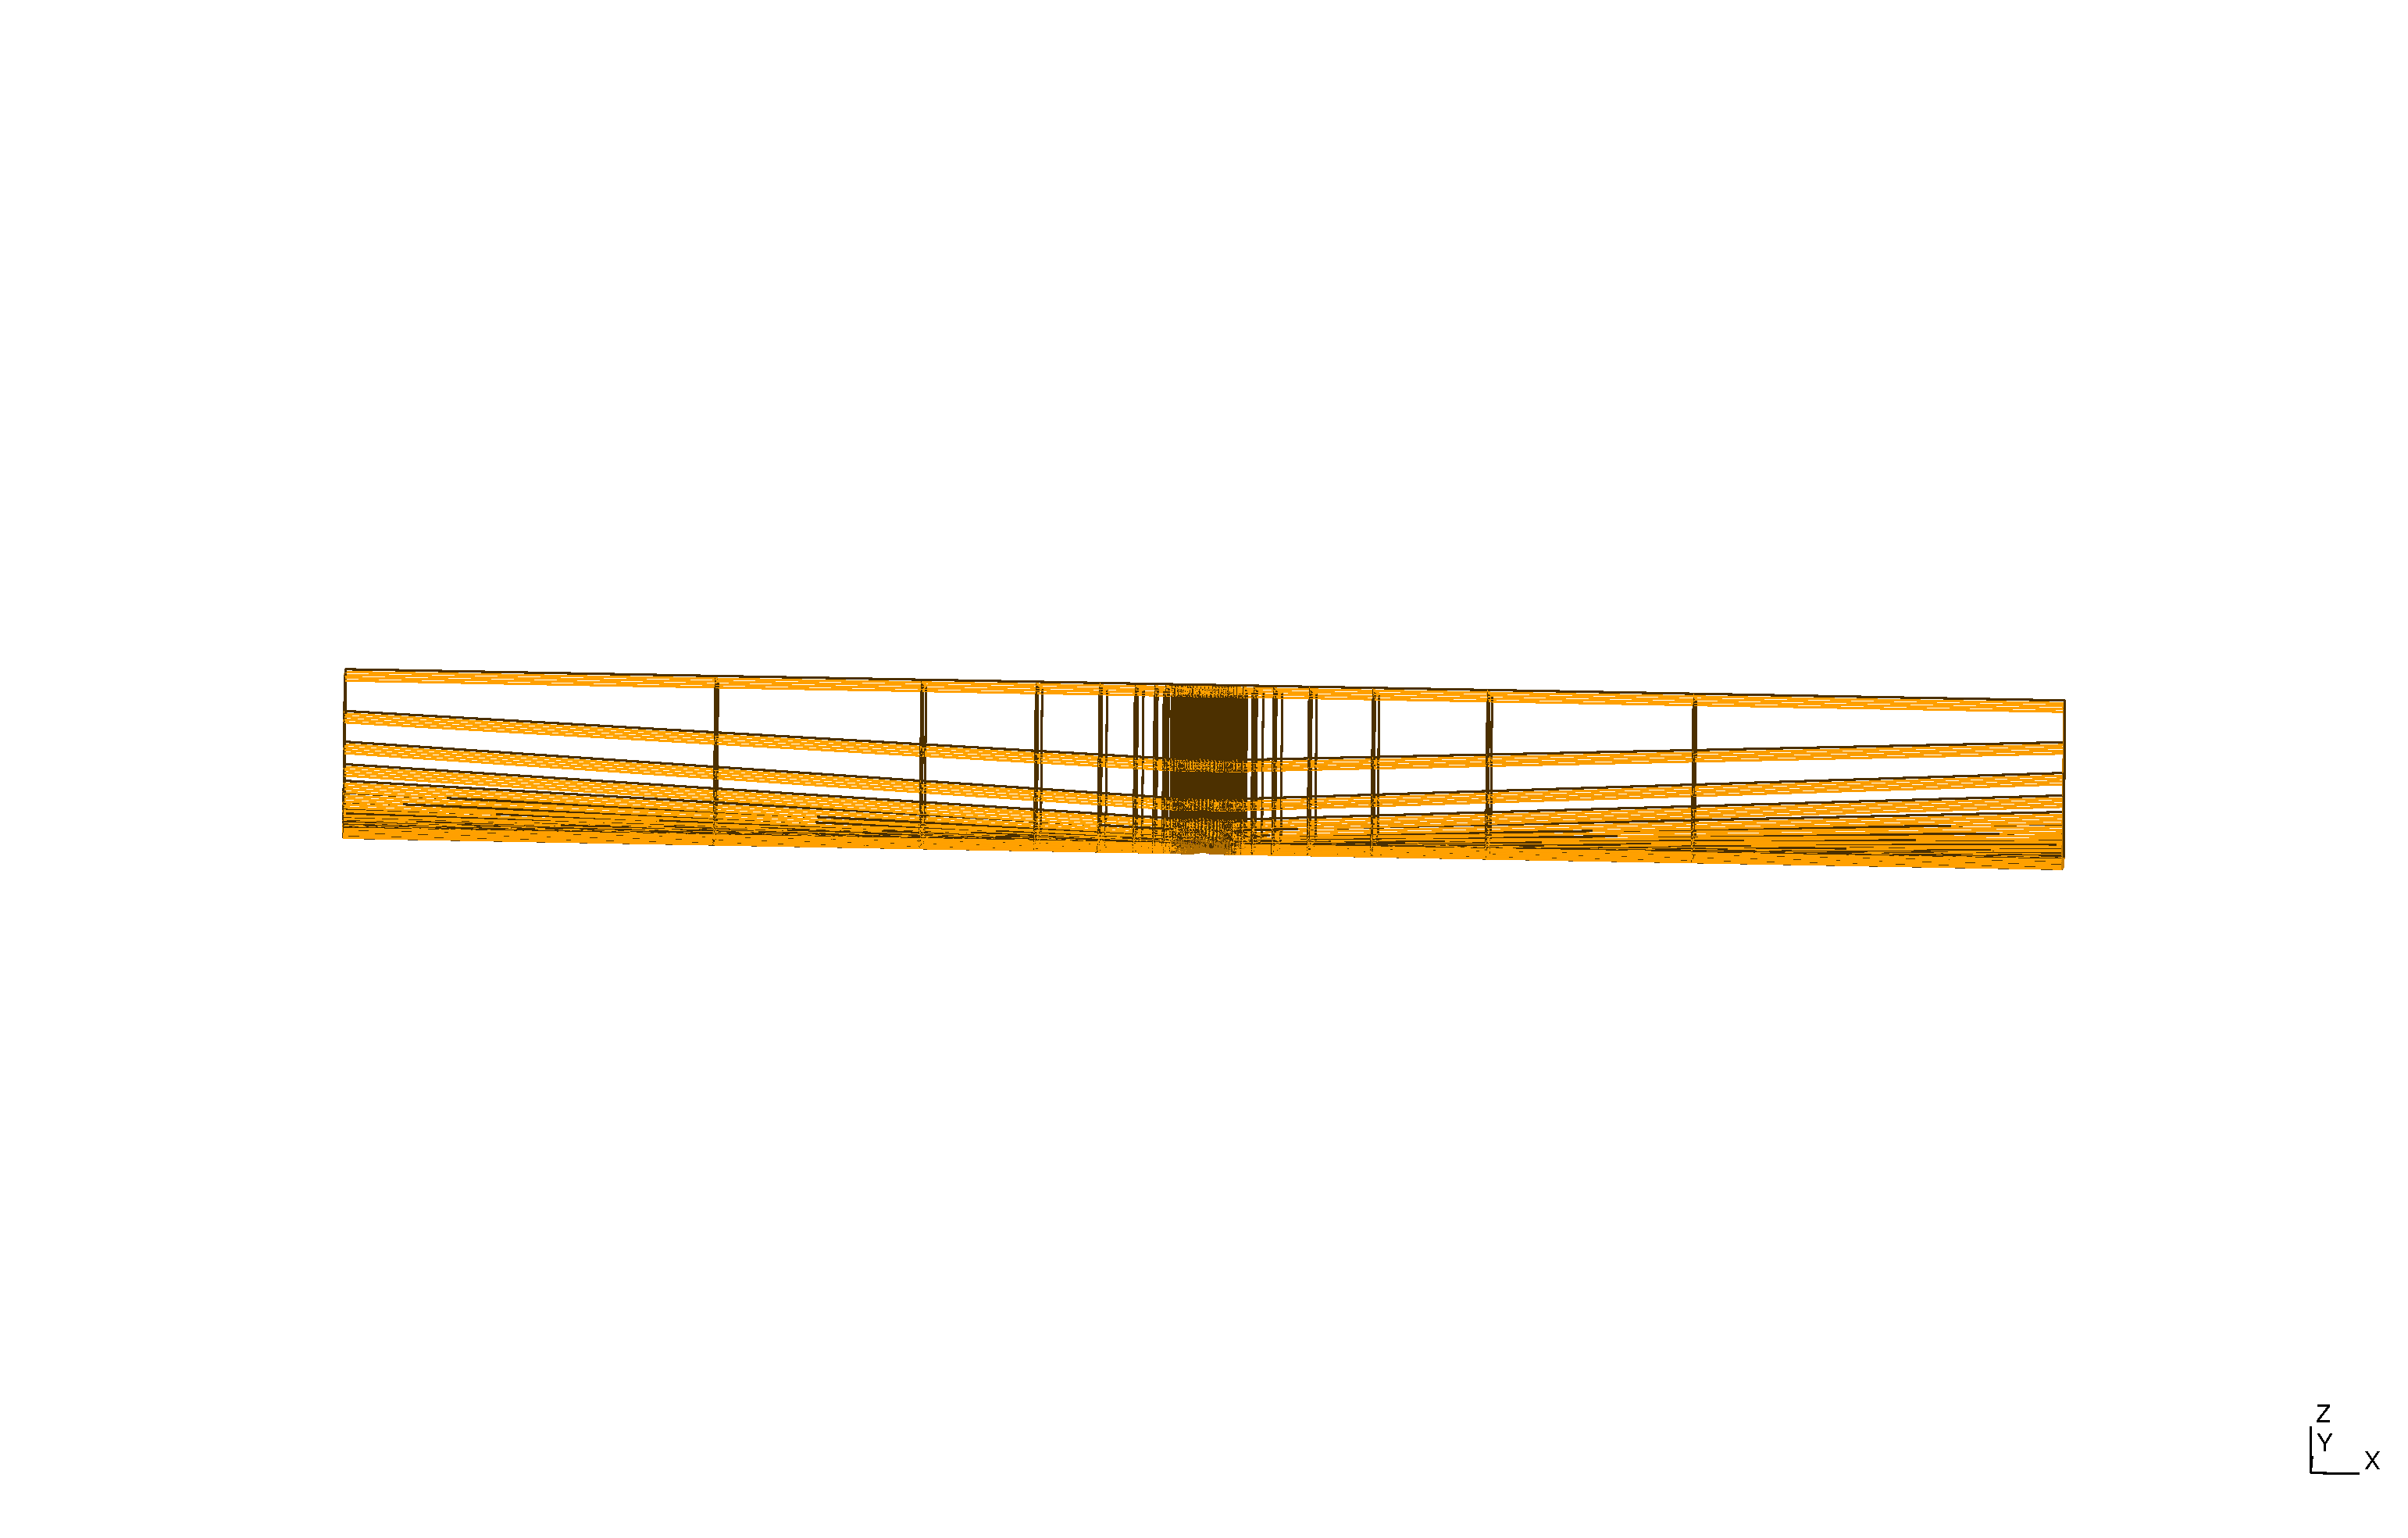
\includegraphics[scale=0.3]{bump3d-vcoarse2}
 \caption{Coarsest curved mesh of 3D bump}
 \label{fig:bump3d}
\end{figure}

\begin{figure}
	\centering
	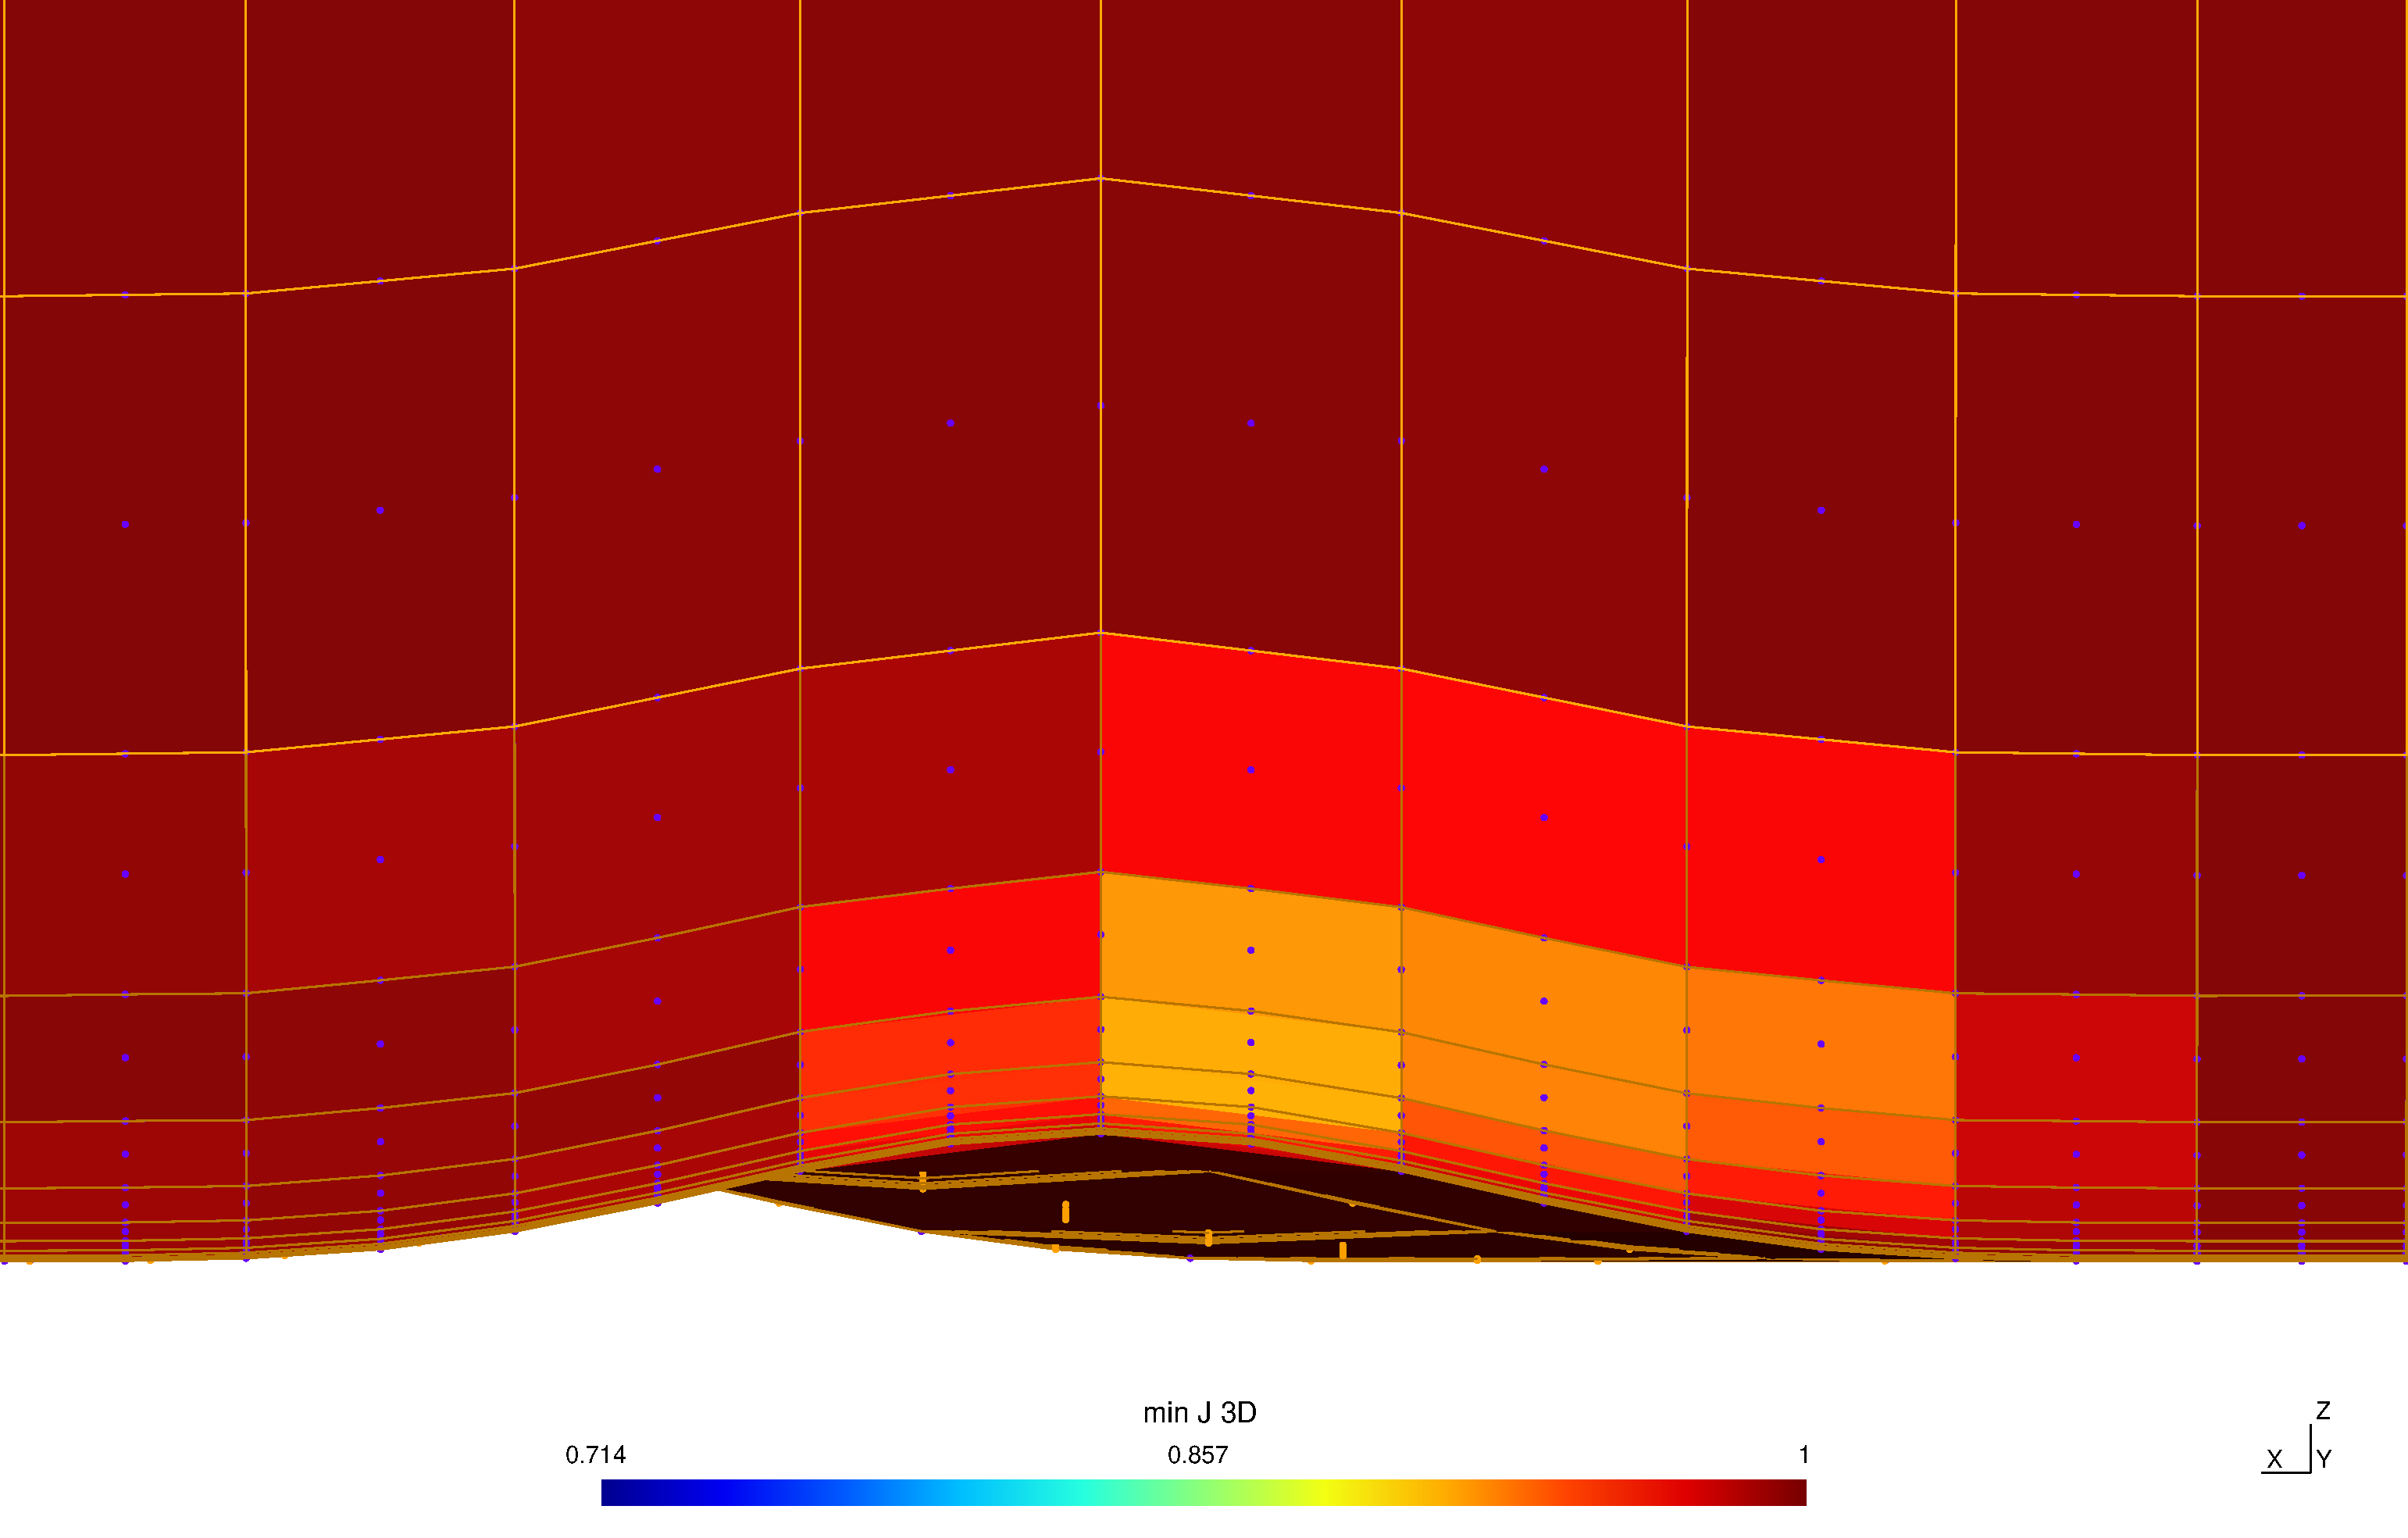
\includegraphics[width=400pt,scale=0.5]{bump3d-vcoarse-quality}
	\caption{Minimum scaled Jacobian of coarse curved mesh of 3D bump}
	\label{fig:bump3d-coarse-jac}
\end{figure}
\begin{figure}
	\centering
	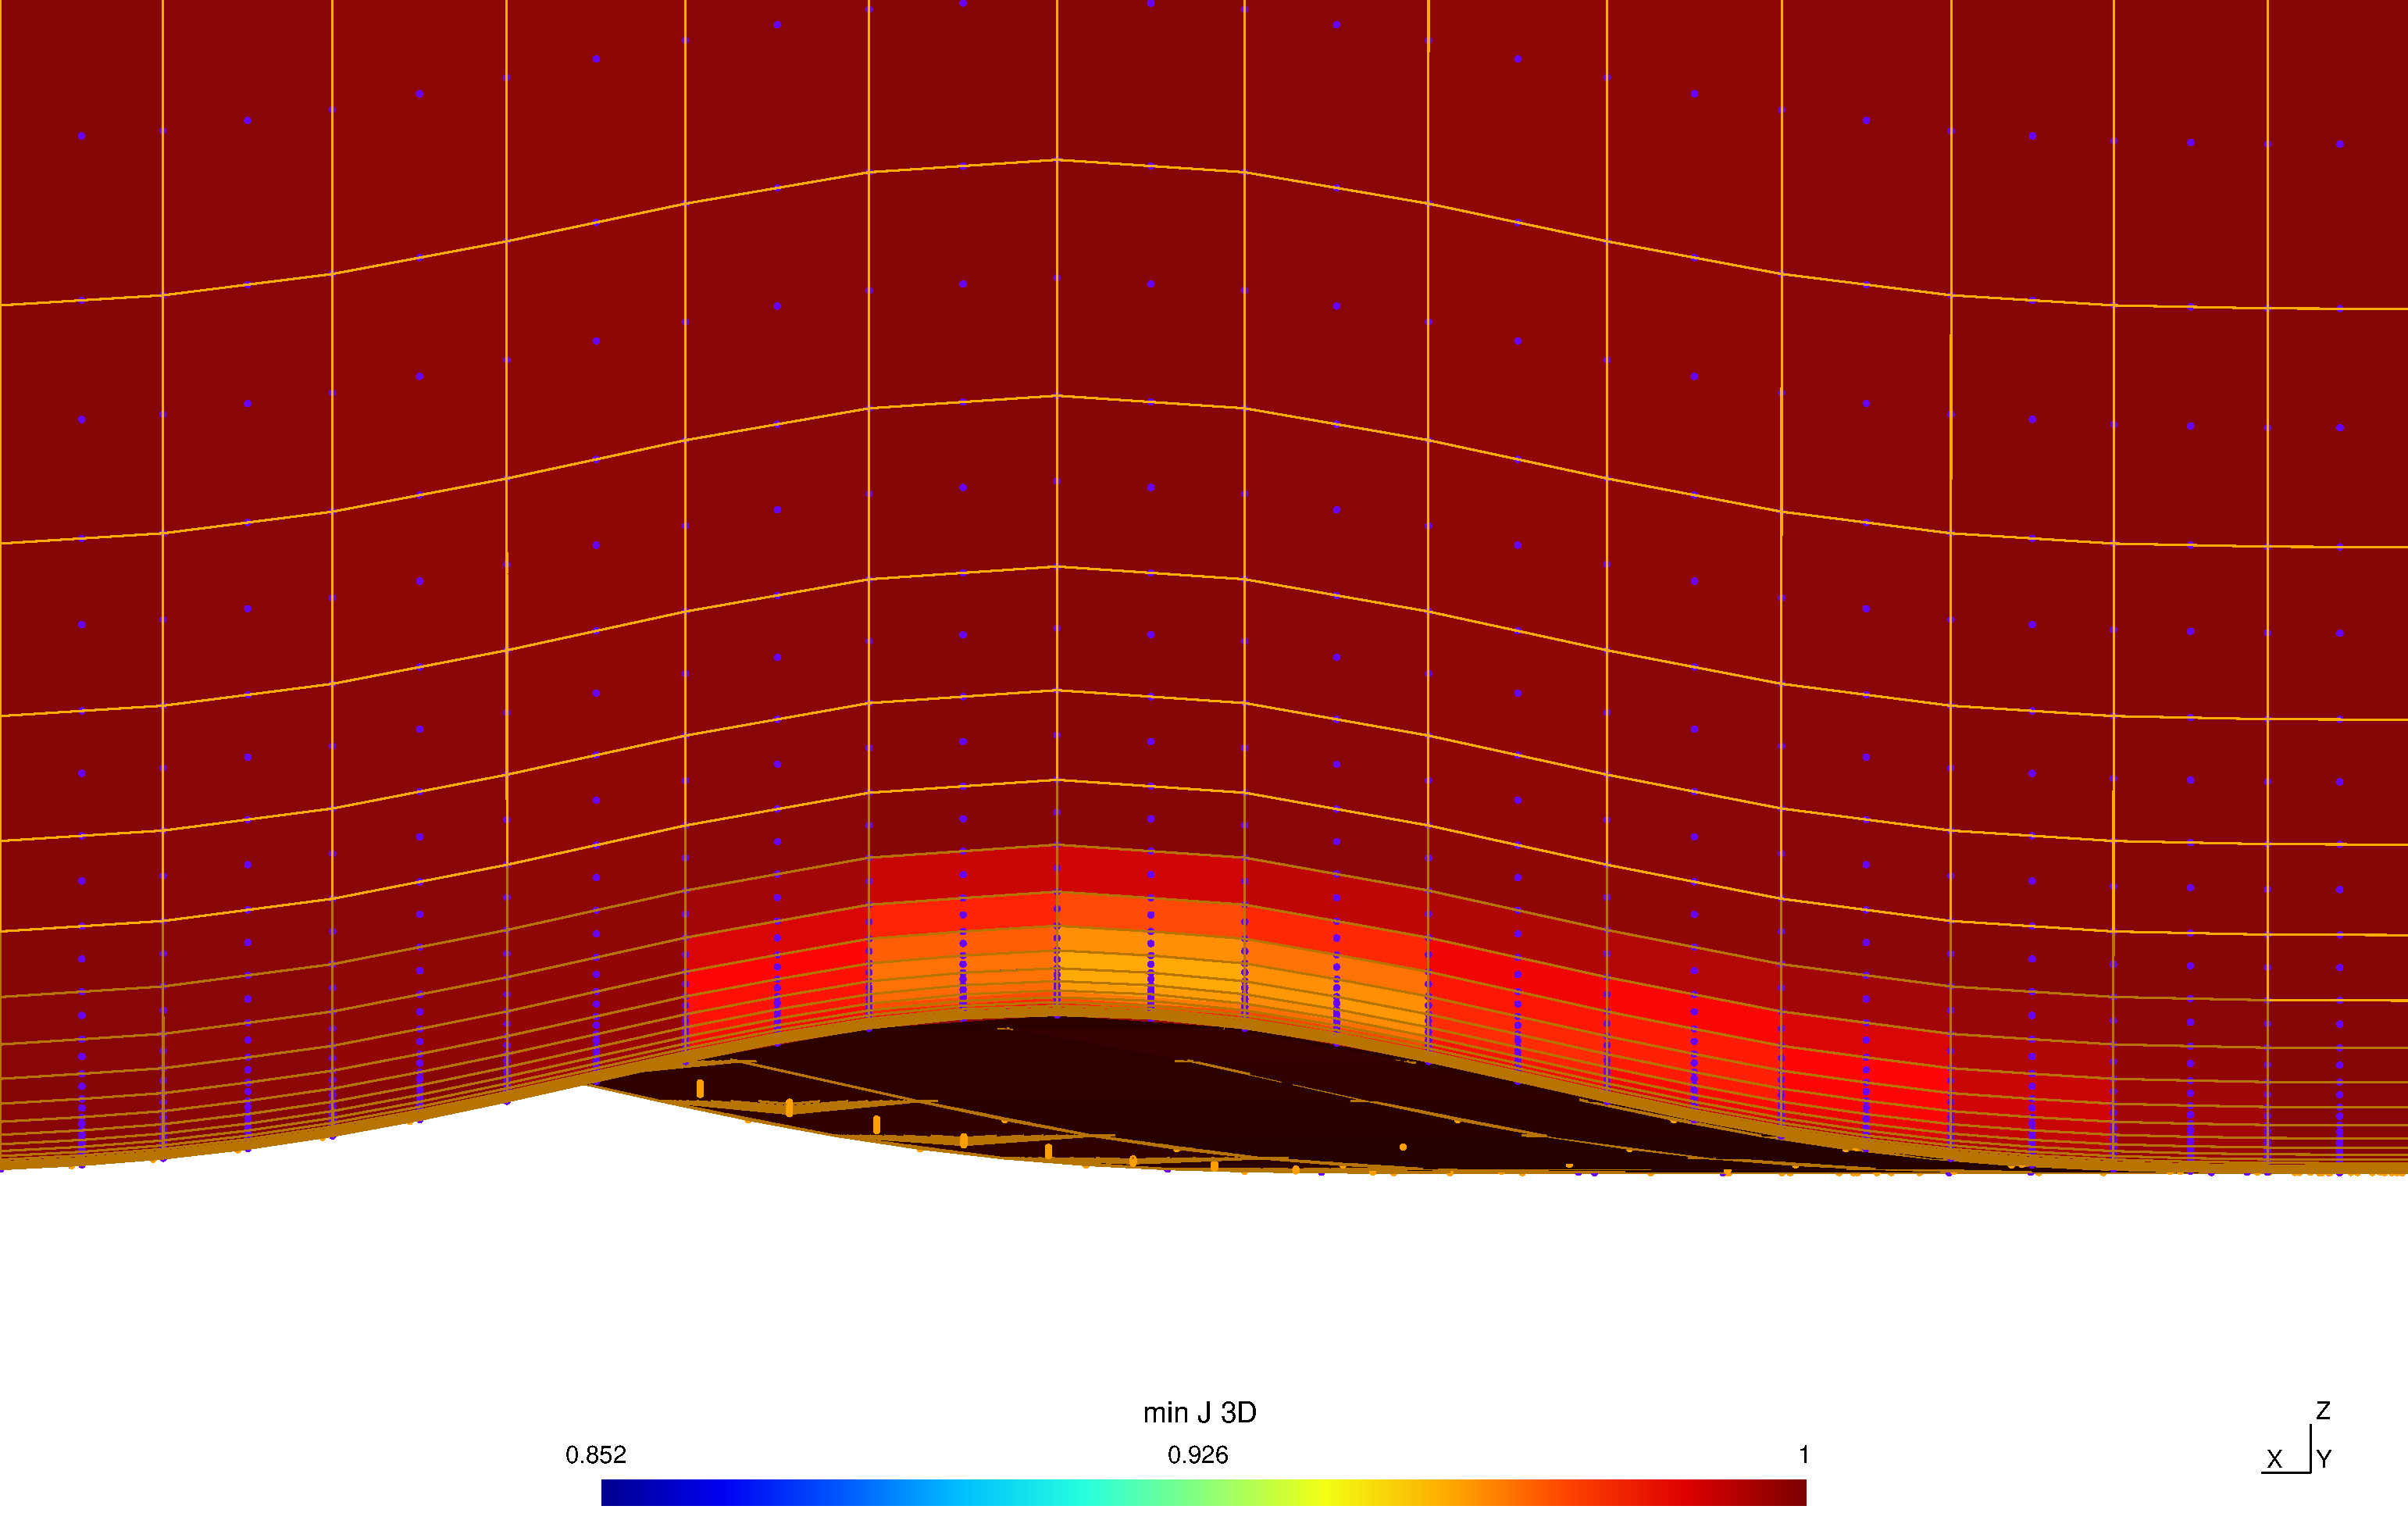
\includegraphics[width=400pt,scale=0.5]{bump3d-medium-quality}
	\caption{Minimum scaled Jacobian of medium curved mesh of 3D bump}
	\label{fig:bump3d-medium-jac}
\end{figure}

Further, we present results from NC State University's reconstructed discontinuous Galerkin turbulent flow code RDGFLO run on the curved meshes. A DG P1 scheme with Taylor basis, HLLC inviscid flux, Bassi-Rebay 2 (BR2) viscous flux, and first-order implicit time integration using Newton linearization and LU-SGS preconditioned GMRES solver is used for obtaining the solution; we refer to Liu et. al. for details \cite{solver}. For comparison, the result obtained from a curved mesh formed by agglomeration of a finer mesh is also shown. This is to show that the generated curved meshes actually work well when used for running simulations. The convergence of the mass-flux residual with time steps is shown in figure \ref{fig:resconvergence}.
\begin{figure}
	\centering
	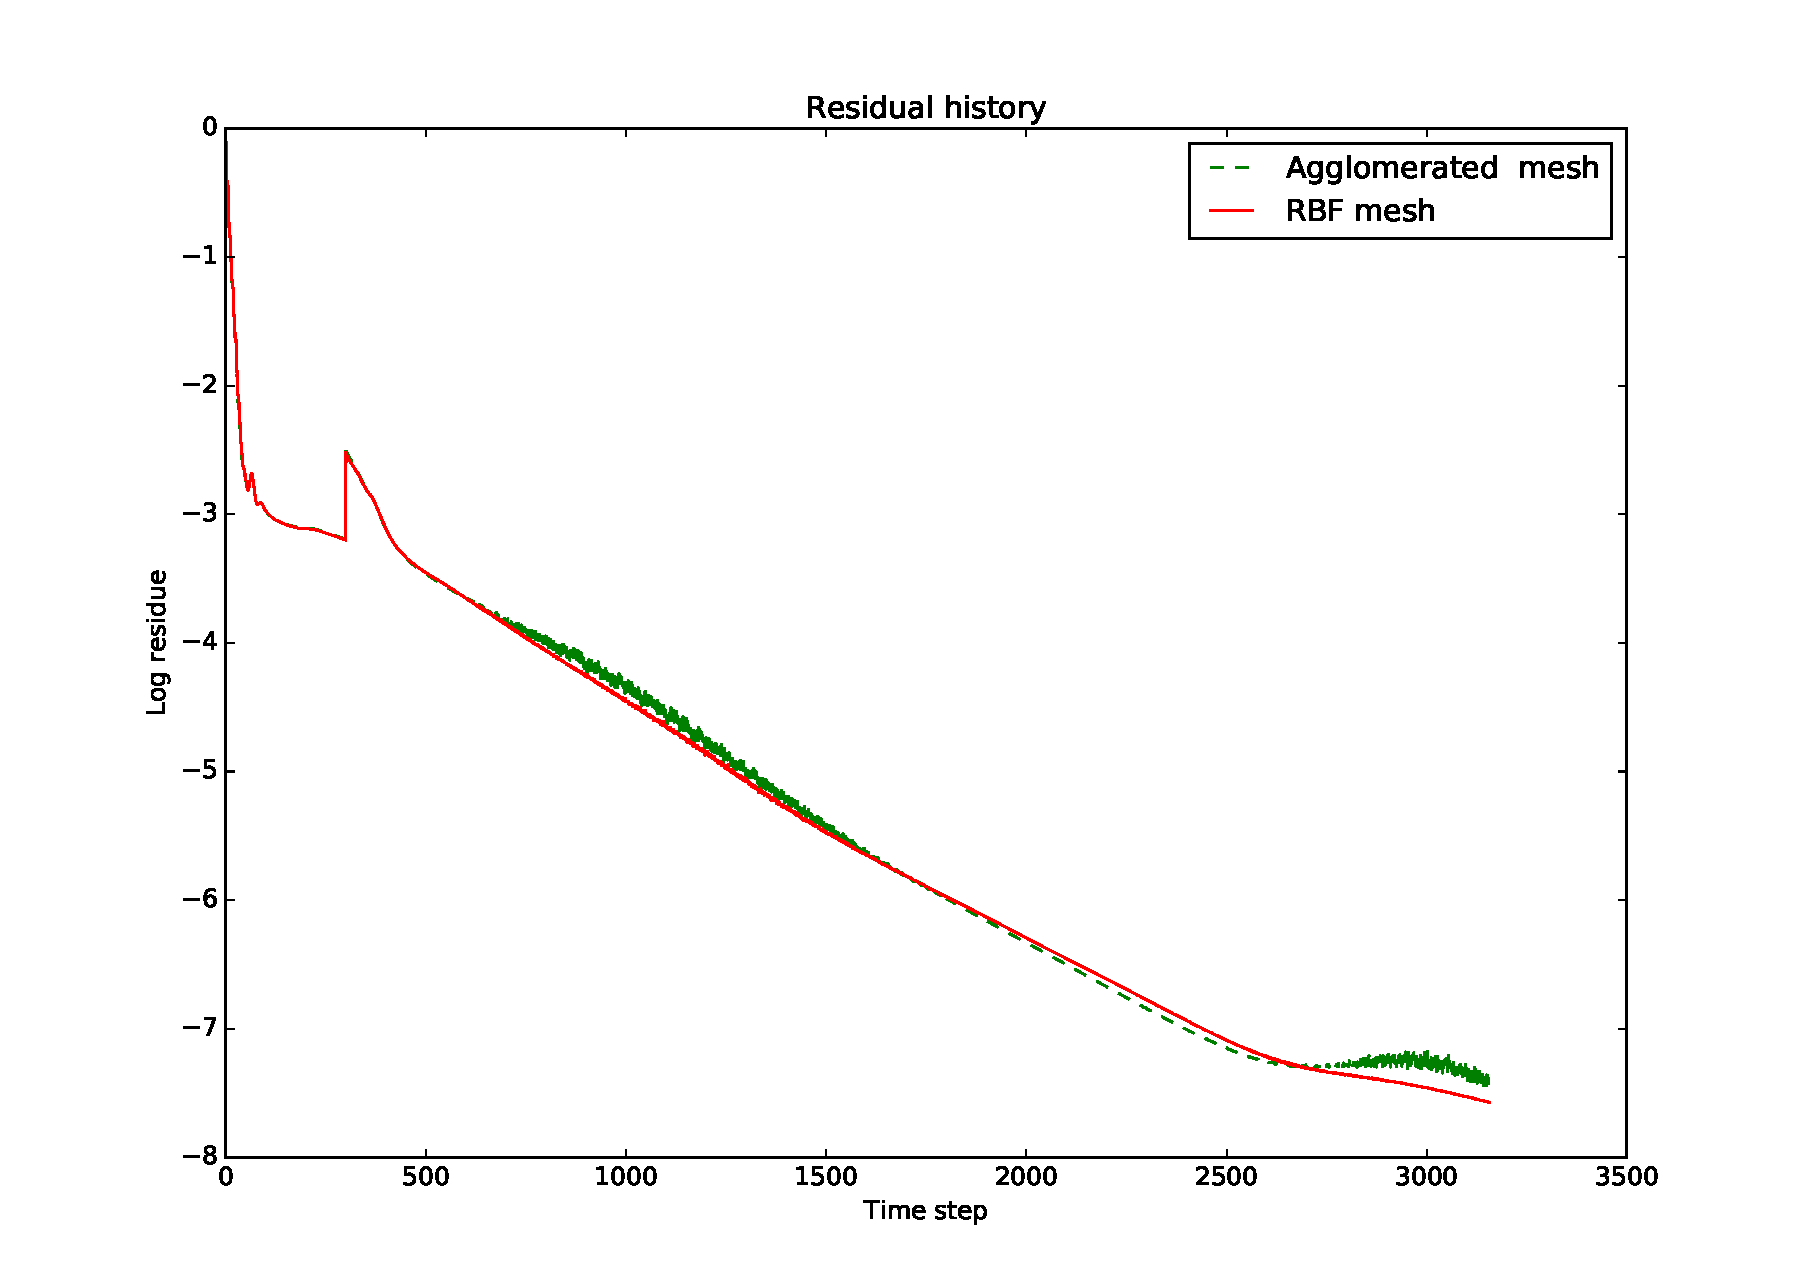
\includegraphics[scale=0.5]{solver-convergence}
	\caption{Comparison of mass-flux residual convergence history with time steps for implicit DG P1 solution}
	\label{fig:resconvergence}
\end{figure}
\chapter{Conclusions and Future Work}

A lot of choice is available for mesh-movement techniques, but only a few will be good for a given application. We conclude that interpolation methods are generally well-suited for unsteady simulations that require mesh movement, as they are very fast. When deformations are relatively small and not highly rotational, DGM is a good choice while when larger and more general deformations are needed, DGRBF is best. The pure RBF method, while usually giving good robust results, is more expensive than other interpolation methods considered here. 

RBF, and to some extent linear elasticity methods, are found to be effective for curved mesh generation, where computational cost is less of an issue. We have used RBF for curved mesh generation with good results for certain viscous flow cases.

One direction for future work is to complete a surface reconstruction procedure in 3D. For some meshes, the requirement of global $C^2$ continuity is too restrictive. Also, a procedure similar to that described in section \ref{subsec:spline2d} would be quite expensive for surfaces in $\mathbb{R}^3$. We therefore consider local fittings of 2D Taylor polynomials at every boundary vertex, described in \cite{sr:jiaowang} as ``Weighted Averaging of Local Fittings" (WALF). In their paper, Jiao and Wang fit local 2D Taylor polynomials to each vertex of the surface mesh. The coefficients, that is, the derivatives of a local height function in a local coordinate system centered at the vertex, are solved for using vertex position data from a neighborhood of that vertex. It is ensured that there are more neighboring points being considered for data than the number of unknowns to solve for, thereby obtaining an over-determined system of equations. This is solved by a weighted least-squares approach. This is claimed to work well for both smooth surfaces and surfaces with $C^1$ discontinuities (ridges, corners etc.). For the latter case, additional preprocessing of the linear surface mesh is required to detect discontinuities \cite{sr:discontinuities}.




%%---------------------------------------------------------------------------%%
%%  Bibliography 

%%  You can use the bibitem list.
%\bibliographystyle{unsrt}
%\begin{thebibliography}{99}
%\bibitem{cb02}
%Casella, G. and Berger, R.L. (2002)
%\newblock {\it Statistical Inference, Second Edition.}
%Duxbury Press, Belmont, CA.
%
%\bibitem{t06}
%Tsiatis, A.A. (2006)
%\newblock {\it Semiparametric Theory and Missing Data.}
%Springer, New York.
%
%\end{thebibliography}

%% or use BibTeX
\bibliography{AdityaKashi-thesis}{}
\bibliographystyle{plain}

%%---------------------------------------------------------------------------%%
% Appendices
\appendix

\chapter{Delaunay tessellation algorithm}

Here, the exact algorithm used for the Delaunay tessellation in the context of Delaunay graph mapping (DGM) methods is explained. The method broadly follows the one used by Bowyer \cite{bowyer}. 

The Delaunay process maximizes the minimum angle in a simplex. Implementation of the ``Delaunay kernel" is done such that orientation of elements and faces is preserved.

\chapter[Spline reconstruction]{Spline reconstruction of a piecewise-linear boundary}
\label{app:spline}

The exact process used to reconstruct a twice-differentiable ($C^2$) boundary from the piecewise-linear boundary of a linear 2D mesh is described. Each one-dimensional boundary facet of the two-dimensional mesh is reconstructed into a cubic spline. The basic framework of the method is taken from \cite{sr:wolframspline}. We assume there are $N$ boundary facets and thus $N+1$ boundary nodes.

We want to reconstruct the $i$th boundary facet into a curve in $\mathbb{R}^2$ as
\begin{eqnarray}
\bld{r}_i(t) &=& \bld{a}_i + \bld{b}_i t + \bld{c}_it^2 + \bld{d}_it^3, \quad t \in [0,1]
%\bld{r}_i'(t) &=& \bld{b}_i + 2\bld{c}_it + 3\bld{d}_it^2 \\
%\bld{r}_i''(t) &=& 2\bld{c}_i + 6\bld{d}_it
\end{eqnarray}
$t=0$ corresponds to the starting point of the boundary facet while $t=1$ corresponds to the ending point. We impose $C^0$, $C^1$ and $C^2$ continuity of the curve to form a square linear system. That is, for all $i \in \{0,1,...,N\}$
\begin{eqnarray}
\bld{r}_i(0) &=& \bld{R}_i \\
\bld{r}_i(1) &=& \bld{R}_{i+1} \\
\bld{r}_i'(0) &=& \bld{r}_{i-1}'(1) \\
\bld{r}_i'(1) &=& \bld{r}_{i+1}'(0) \\
\bld{r}_i''(0) &=& \bld{r}_{i-1}''(1) \\
\bld{r}_i''(1) &=& \bld{r}_{i+1}''(0)
\end{eqnarray}
where $\bld{R}_i$ denotes the coordinates of the $i$th boundary point. The ``boundary conditions'' are, in case of a closed curve,
\begin{eqnarray}
\bld{R}_0 &=& \bld{R}_{N+1} \\
\bld{r}_0'(0) &=& \bld{r}_N'(1) \\
\bld{r}_0''(0) &=& \bld{r}_N''(1)
\end{eqnarray}
and in case of an open curve
\begin{eqnarray}
\bld{r}_0''(0) &=& 0 \\
\bld{r}_N''(1) &=& 0.
\end{eqnarray}

For assembling the 3 systems of equations for the x-, y- and z-components of the spline curve, we define $D_i := r_i'(0) \, \forall \, i \in \{1,2,...,N\}$ and $D_{N+1} := r_N'(1)$ where $r$ is $x$, $y$ and $z$ in turn. We express the coefficients $a_i$, $b_i$, $c_i$ and $d_i$ in terms of the $D_i$ and $R_i$ (the coordinates of boundary nodes). Finally, we obtain, for an open curve
\begin{equation}
\begin{bmatrix}
2 & 1 & & & & & \\
 & 1 & 4 & 1 & & & \\
 & & \ddots & \ddots & \ddots & &\\
 & & & & 1 & 4 & 1 \\
 & & & & & 1 & 2
\end{bmatrix}
\begin{bmatrix}
D_1 \\
D_2 \\
\vdots \\
D_N \\
D_{N+1}
\end{bmatrix}
=
\begin{bmatrix}
3(r_2 - r_1) \\
3(r_3 - r_1) \\
\vdots \\
3(r_{N+1}-r_{N-1}) \\
3(r_{N+1} - r_N)
\end{bmatrix}.
\end{equation}
After a similar derivation, for a closed curve we obtain
\begin{equation}
\begin{bmatrix}
4 & 1 & & & & 1 & 0 \\
& 1 & 4 & 1 & & & \\
& & \ddots & \ddots & \ddots & &\\
& & & & 1 & 4 & 1 \\
0 &1 & & & & 1 & 4
\end{bmatrix}
\begin{bmatrix}
D_1 \\
D_2 \\
\vdots \\
D_N \\
D_{N+1}
\end{bmatrix}
=
\begin{bmatrix}
3(r_2 - r_{N}) \\
3(r_3 - r_1) \\
\vdots \\
3(r_{N+1}-r_{N-1}) \\
3(r_2 - r_N)
\end{bmatrix}.
\end{equation}




%%---------------------------------------------------------------------------%%
\backmatter


\end{document}
